% Options for packages loaded elsewhere
\PassOptionsToPackage{unicode}{hyperref}
\PassOptionsToPackage{hyphens}{url}
%
\documentclass[
]{book}
\usepackage{amsmath,amssymb}
\usepackage{iftex}
\ifPDFTeX
  \usepackage[T1]{fontenc}
  \usepackage[utf8]{inputenc}
  \usepackage{textcomp} % provide euro and other symbols
\else % if luatex or xetex
  \usepackage{unicode-math} % this also loads fontspec
  \defaultfontfeatures{Scale=MatchLowercase}
  \defaultfontfeatures[\rmfamily]{Ligatures=TeX,Scale=1}
\fi
\usepackage{lmodern}
\ifPDFTeX\else
  % xetex/luatex font selection
\fi
% Use upquote if available, for straight quotes in verbatim environments
\IfFileExists{upquote.sty}{\usepackage{upquote}}{}
\IfFileExists{microtype.sty}{% use microtype if available
  \usepackage[]{microtype}
  \UseMicrotypeSet[protrusion]{basicmath} % disable protrusion for tt fonts
}{}
\makeatletter
\@ifundefined{KOMAClassName}{% if non-KOMA class
  \IfFileExists{parskip.sty}{%
    \usepackage{parskip}
  }{% else
    \setlength{\parindent}{0pt}
    \setlength{\parskip}{6pt plus 2pt minus 1pt}}
}{% if KOMA class
  \KOMAoptions{parskip=half}}
\makeatother
\usepackage{xcolor}
\usepackage{color}
\usepackage{fancyvrb}
\newcommand{\VerbBar}{|}
\newcommand{\VERB}{\Verb[commandchars=\\\{\}]}
\DefineVerbatimEnvironment{Highlighting}{Verbatim}{commandchars=\\\{\}}
% Add ',fontsize=\small' for more characters per line
\usepackage{framed}
\definecolor{shadecolor}{RGB}{248,248,248}
\newenvironment{Shaded}{\begin{snugshade}}{\end{snugshade}}
\newcommand{\AlertTok}[1]{\textcolor[rgb]{0.94,0.16,0.16}{#1}}
\newcommand{\AnnotationTok}[1]{\textcolor[rgb]{0.56,0.35,0.01}{\textbf{\textit{#1}}}}
\newcommand{\AttributeTok}[1]{\textcolor[rgb]{0.13,0.29,0.53}{#1}}
\newcommand{\BaseNTok}[1]{\textcolor[rgb]{0.00,0.00,0.81}{#1}}
\newcommand{\BuiltInTok}[1]{#1}
\newcommand{\CharTok}[1]{\textcolor[rgb]{0.31,0.60,0.02}{#1}}
\newcommand{\CommentTok}[1]{\textcolor[rgb]{0.56,0.35,0.01}{\textit{#1}}}
\newcommand{\CommentVarTok}[1]{\textcolor[rgb]{0.56,0.35,0.01}{\textbf{\textit{#1}}}}
\newcommand{\ConstantTok}[1]{\textcolor[rgb]{0.56,0.35,0.01}{#1}}
\newcommand{\ControlFlowTok}[1]{\textcolor[rgb]{0.13,0.29,0.53}{\textbf{#1}}}
\newcommand{\DataTypeTok}[1]{\textcolor[rgb]{0.13,0.29,0.53}{#1}}
\newcommand{\DecValTok}[1]{\textcolor[rgb]{0.00,0.00,0.81}{#1}}
\newcommand{\DocumentationTok}[1]{\textcolor[rgb]{0.56,0.35,0.01}{\textbf{\textit{#1}}}}
\newcommand{\ErrorTok}[1]{\textcolor[rgb]{0.64,0.00,0.00}{\textbf{#1}}}
\newcommand{\ExtensionTok}[1]{#1}
\newcommand{\FloatTok}[1]{\textcolor[rgb]{0.00,0.00,0.81}{#1}}
\newcommand{\FunctionTok}[1]{\textcolor[rgb]{0.13,0.29,0.53}{\textbf{#1}}}
\newcommand{\ImportTok}[1]{#1}
\newcommand{\InformationTok}[1]{\textcolor[rgb]{0.56,0.35,0.01}{\textbf{\textit{#1}}}}
\newcommand{\KeywordTok}[1]{\textcolor[rgb]{0.13,0.29,0.53}{\textbf{#1}}}
\newcommand{\NormalTok}[1]{#1}
\newcommand{\OperatorTok}[1]{\textcolor[rgb]{0.81,0.36,0.00}{\textbf{#1}}}
\newcommand{\OtherTok}[1]{\textcolor[rgb]{0.56,0.35,0.01}{#1}}
\newcommand{\PreprocessorTok}[1]{\textcolor[rgb]{0.56,0.35,0.01}{\textit{#1}}}
\newcommand{\RegionMarkerTok}[1]{#1}
\newcommand{\SpecialCharTok}[1]{\textcolor[rgb]{0.81,0.36,0.00}{\textbf{#1}}}
\newcommand{\SpecialStringTok}[1]{\textcolor[rgb]{0.31,0.60,0.02}{#1}}
\newcommand{\StringTok}[1]{\textcolor[rgb]{0.31,0.60,0.02}{#1}}
\newcommand{\VariableTok}[1]{\textcolor[rgb]{0.00,0.00,0.00}{#1}}
\newcommand{\VerbatimStringTok}[1]{\textcolor[rgb]{0.31,0.60,0.02}{#1}}
\newcommand{\WarningTok}[1]{\textcolor[rgb]{0.56,0.35,0.01}{\textbf{\textit{#1}}}}
\usepackage{longtable,booktabs,array}
\usepackage{calc} % for calculating minipage widths
% Correct order of tables after \paragraph or \subparagraph
\usepackage{etoolbox}
\makeatletter
\patchcmd\longtable{\par}{\if@noskipsec\mbox{}\fi\par}{}{}
\makeatother
% Allow footnotes in longtable head/foot
\IfFileExists{footnotehyper.sty}{\usepackage{footnotehyper}}{\usepackage{footnote}}
\makesavenoteenv{longtable}
\usepackage{graphicx}
\makeatletter
\def\maxwidth{\ifdim\Gin@nat@width>\linewidth\linewidth\else\Gin@nat@width\fi}
\def\maxheight{\ifdim\Gin@nat@height>\textheight\textheight\else\Gin@nat@height\fi}
\makeatother
% Scale images if necessary, so that they will not overflow the page
% margins by default, and it is still possible to overwrite the defaults
% using explicit options in \includegraphics[width, height, ...]{}
\setkeys{Gin}{width=\maxwidth,height=\maxheight,keepaspectratio}
% Set default figure placement to htbp
\makeatletter
\def\fps@figure{htbp}
\makeatother
\setlength{\emergencystretch}{3em} % prevent overfull lines
\providecommand{\tightlist}{%
  \setlength{\itemsep}{0pt}\setlength{\parskip}{0pt}}
\setcounter{secnumdepth}{5}
\usepackage{booktabs}
\usepackage{booktabs}
\usepackage{caption}
\usepackage{longtable}
\usepackage{colortbl}
\usepackage{array}
\usepackage{anyfontsize}
\usepackage{multirow}
\ifLuaTeX
  \usepackage{selnolig}  % disable illegal ligatures
\fi
\usepackage[]{natbib}
\bibliographystyle{plainnat}
\usepackage{bookmark}
\IfFileExists{xurl.sty}{\usepackage{xurl}}{} % add URL line breaks if available
\urlstyle{same}
\hypersetup{
  pdftitle={Atlas interactif des dynamiques environnementales en Afrique de l'Ouest},
  pdfauthor={Ahmadou Niass \& Samba Sow},
  hidelinks,
  pdfcreator={LaTeX via pandoc}}

\title{Atlas interactif des dynamiques environnementales en Afrique de l'Ouest}
\author{Ahmadou Niass \& Samba Sow}
\date{2025-04-16}

\begin{document}
\maketitle

{
\setcounter{tocdepth}{1}
\tableofcontents
}
\chapter{Présentation du projet}\label{pruxe9sentation-du-projet}

Ce document présente l'Atlas Spectral du Sahel, un outil interactif d'analyse environnementale reposant sur des indices spectraux dérivés d'images satellites. Construit avec Bookdown et articulé autour de visualisations dynamiques, cet atlas propose une lecture spatiale et temporelle des dynamiques écologiques en Afrique de l'Ouest, avec un focus sur quatre pays : le Sénégal, le Burkina Faso, le Niger et le Mali.

L'objectif principal de ce travail est de mettre en lumière les contrastes environnementaux, les transitions écologiques et les zones sensibles à partir d'indicateurs spectraux synthétiques. Les données utilisées proviennent de traitements d'images multispectrales (Sentinel-2, Landsat), agrégées sous forme de rasters régionaux à haute résolution, puis intégrées dans un environnement interactif pour faciliter la visualisation, l'analyse comparative et l'interprétation.

\section{Objectifs de l'atlas}\label{objectifs-de-latlas}

Cet atlas vise à :

Suivre les dynamiques végétales à travers des indices comme le NDVI (végétation verte), le SAVI ou l'ARVI ;

Détecter les zones de stress ou de dégradation écologique via des indices sensibles comme l'ARI ou le BAI ;

Évaluer la santé physiologique de la végétation et sa capacité à résister aux perturbations climatiques ;

Cartographier les zones humides et les gradients d'humidité des sols à travers des indices comme le LSWI, l'ANDWI ou le WI2 ;

Offrir une plateforme de lecture claire et reproductible des dynamiques environnementales à l'échelle infranationale.

\section{Méthodologie}\label{muxe9thodologie}

Chaque indice spectral repose sur une combinaison spécifique de bandes du spectre optique (rouge, vert, infrarouge, etc.) et permet de caractériser une propriété écologique ou biophysique. Les rasters ont été traités et standardisés, puis agrégés à l'échelle des régions administratives, pour permettre une lecture multi-échelles (locale, nationale, régionale).

Les cartes présentées dans chaque chapitre ont été générées à l'aide de Leaflet (pour les visualisations interactives) et de tmap (pour les rendus statiques). Une attention particulière a été portée à l'esthétique, à l'harmonisation des palettes de couleurs et à la précision des découpages administratifs.`

Les images satellites ont été pré-traitées et les indices calculés à l'aide de \textbf{packages R spécialisés}, notamment :

\begin{Shaded}
\begin{Highlighting}[]
\FunctionTok{library}\NormalTok{(sf)}
\FunctionTok{library}\NormalTok{(raster)}
\FunctionTok{library}\NormalTok{(terra)}
\FunctionTok{library}\NormalTok{(tmap)}
\FunctionTok{library}\NormalTok{(leaflet)}
\FunctionTok{library}\NormalTok{(tidyverse)}
\FunctionTok{library}\NormalTok{(exactextractr)}
\FunctionTok{library}\NormalTok{(gtsummary)}
\end{Highlighting}
\end{Shaded}

Les valeurs ont ensuite été agrégées \textbf{par région administrative} à l'aide de shapefiles standardisés (\texttt{shapes/}), permettant une comparaison cohérente à travers les pays.

\begin{center}\rule{0.5\linewidth}{0.5pt}\end{center}

\section{Structure du livre}\label{structure-du-livre}

Le Bookdown est divisé en \textbf{quatre grands chapitres}, chacun dédié à un pays :

\begin{enumerate}
\def\labelenumi{\arabic{enumi}.}
\tightlist
\item
  \textbf{Chapitre 1 -- Sénégal}\\
\item
  \textbf{Chapitre 2 -- Burkina Faso}\\
\item
  \textbf{Chapitre 3 -- Niger}\\
\item
  \textbf{Chapitre 4 -- Mali}
\end{enumerate}

Chaque chapitre présente :
- Les \textbf{cartes thématiques} (par indicateur et par année)
- Les \textbf{profils d'évolution temporelle} par région
- Des \textbf{comparaisons spatiales} et \textbf{interprétations environnementales}

\begin{center}\rule{0.5\linewidth}{0.5pt}\end{center}

\section{À qui s'adresse ce projet ?}\label{uxe0-qui-sadresse-ce-projet}

\begin{itemize}
\tightlist
\item
  Aux \textbf{étudiants} en statistique, environnement, géomatique ;
\item
  Aux \textbf{enseignants-chercheurs} explorant les outils open source en analyse spatiale ;
\item
  Aux \textbf{décideurs} souhaitant disposer d'un appui analytique régional ;
\item
  À toute personne curieuse de comprendre les \textbf{mutations écologiques} du Sahel.
\end{itemize}

\begin{center}\rule{0.5\linewidth}{0.5pt}\end{center}

\section{Remerciements}\label{remerciements}

Nous adressons nos remerciements à \textbf{M. Aboubacar Hema} pour son accompagnement rigoureux, ses suggestions méthodologiques et son engagement pour une formation appliquée et innovante.

\begin{center}\rule{0.5\linewidth}{0.5pt}\end{center}

\section{Commencez l'exploration 🌍}\label{commencez-lexploration}

Ce livre vous invite à \textbf{explorer, comparer et interpréter les dynamiques écologiques} de l'Afrique de l'Ouest à travers les indices spectraux.\\
Bonne lecture, et surtout, \textbf{bonne exploration} !

\begin{quote}
\emph{``Ce n'est qu'en observant les territoires dans leur complexité spatiale que l'on peut éclairer les politiques publiques et favoriser un développement durable ancré dans la réalité des terrains.''}
\end{quote}

\chapter{Sénégal}\label{suxe9nuxe9gal}

\section{Introduction}\label{introduction}

Le Sénégal occupe une position géographique stratégique à la croisée des écosystèmes sahéliens, savaniens et tropicaux. Ce pays présente une diversité écologique remarquable, depuis les zones arides du nord aux forêts humides et galeries fluviales du sud, en passant par les savanes agropastorales du centre. Cette mosaïque d'environnements en fait un terrain d'analyse privilégié pour l'étude des dynamiques végétales, hydriques et climatiques à partir d'indices spectraux.

Dans ce chapitre, nous mobilisons trois grandes familles d'indices issus d'images satellites pour caractériser l'état écologique du territoire sénégalais en 2024 :

Le NDVI (Normalized Difference Vegetation Index) pour mesurer la densité et la vigueur de la végétation verte ;

L'ARI (Anthocyanin Reflectance Index) pour détecter le stress physiologique des plantes, souvent invisible dans les indices classiques ;

Le LSWI (Land Surface Water Index) pour évaluer la teneur en eau des surfaces et la disponibilité hydrique.

Chaque indicateur est analysé à l'échelle régionale, à travers des cartes interactives, des profils statistiques et des interprétations environnementales. Cette approche permet de dégager les régions les plus vulnérables, d'identifier les zones écologiquement stables, et d'alimenter la réflexion sur les politiques de gestion durable des terres et des ressources naturelles.

Ce chapitre constitue ainsi une porte d'entrée vers la compréhension des dynamiques environnementales sahéliennes, en posant les bases d'une analyse comparative approfondie avec les autres pays de l'Atlas.

\begin{center}\rule{0.5\linewidth}{0.5pt}\end{center}

\section{Végétation -- NDVI}\label{vuxe9guxe9tation-ndvi}

Le \textbf{NDVI (Normalized Difference Vegetation Index)} est l'un des indices spectraux les plus utilisés pour l'étude de la végétation. Il permet de mesurer la \textbf{densité et la vigueur de la végétation verte active}, à partir des bandes rouge et proche infrarouge des capteurs satellites.\\
Les valeurs du NDVI s'étendent généralement de --1 à +1, mais dans les milieux naturels, elles se situent entre 0 (sol nu) et 1 (végétation dense).

Dans le cas du Sénégal, nous avons extrait les valeurs \textbf{moyennes du NDVI pour l'année 2024} par région administrative à partir des rasters satellites haute résolution.

\subsection{Carte interactive du NDVI au Sénégal en 2024}\label{carte-interactive-du-ndvi-au-suxe9nuxe9gal-en-2024}

\begin{verbatim}
##   |                                                                              |                                                                      |   0%  |                                                                              |=====                                                                 |   7%  |                                                                              |==========                                                            |  14%  |                                                                              |===============                                                       |  21%  |                                                                              |====================                                                  |  29%  |                                                                              |=========================                                             |  36%  |                                                                              |==============================                                        |  43%  |                                                                              |===================================                                   |  50%  |                                                                              |========================================                              |  57%  |                                                                              |=============================================                         |  64%  |                                                                              |==================================================                    |  71%  |                                                                              |=======================================================               |  79%  |                                                                              |============================================================          |  86%  |                                                                              |=================================================================     |  93%  |                                                                              |======================================================================| 100%
\end{verbatim}

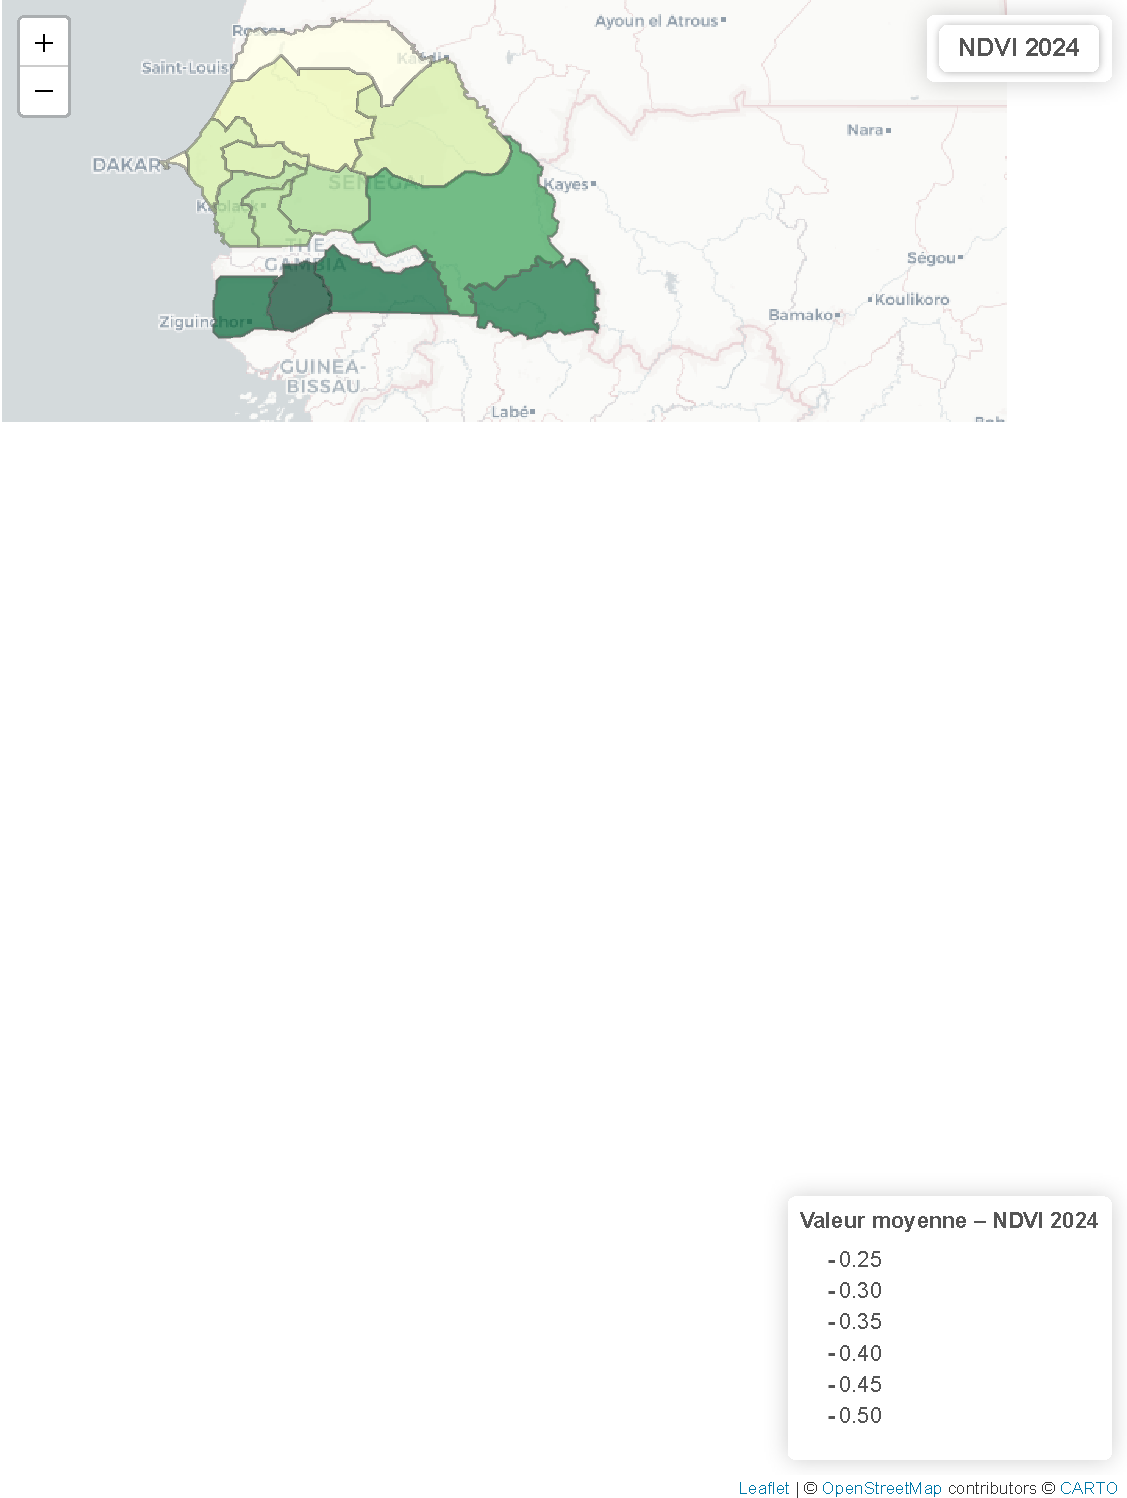
\includegraphics{Atlas-Spectral-Sahel_files/figure-latex/vegetation-ndvi-1.pdf}

\subsection{Tableau de la répartition du NDVI au Sénégal en 2024}\label{tableau-de-la-ruxe9partition-du-ndvi-au-suxe9nuxe9gal-en-2024}

\begin{table}[!t]
\caption*{
{\large \textbf{Moyennes régionales du NDVI}} \\ 
{\small \emph{Sénégal -- Année 2024}}
} 
\fontsize{12.0pt}{14.4pt}\selectfont
\begin{tabular*}{\linewidth}{@{\extracolsep{\fill}}lr}
\toprule
{RÉGION} & {NDVI} \\ 
\midrule\addlinespace[2.5pt]
Dakar & {\cellcolor[HTML]{FBFED0}{\textcolor[HTML]{000000}{0.25}}} \\ 
Diourbel & {\cellcolor[HTML]{D4EEA0}{\textcolor[HTML]{000000}{0.31}}} \\ 
Fatick & {\cellcolor[HTML]{ADDD8E}{\textcolor[HTML]{000000}{0.34}}} \\ 
Kaffrine & {\cellcolor[HTML]{A4D98A}{\textcolor[HTML]{000000}{0.35}}} \\ 
Kaolack & {\cellcolor[HTML]{ADDD8E}{\textcolor[HTML]{000000}{0.34}}} \\ 
Kédougou & {\cellcolor[HTML]{0A6F3A}{\textcolor[HTML]{FFFFFF}{0.47}}} \\ 
Kolda & {\cellcolor[HTML]{006234}{\textcolor[HTML]{FFFFFF}{0.49}}} \\ 
Louga & {\cellcolor[HTML]{ECF8B1}{\textcolor[HTML]{000000}{0.28}}} \\ 
Matam & {\cellcolor[HTML]{D3EDA0}{\textcolor[HTML]{000000}{0.31}}} \\ 
Saint-Louis & {\cellcolor[HTML]{FFFFE5}{\textcolor[HTML]{000000}{0.24}}} \\ 
Sédhiou & {\cellcolor[HTML]{004529}{\textcolor[HTML]{FFFFFF}{0.52}}} \\ 
Tambacounda & {\cellcolor[HTML]{39A156}{\textcolor[HTML]{FFFFFF}{0.42}}} \\ 
Thiès & {\cellcolor[HTML]{D1ED9F}{\textcolor[HTML]{000000}{0.31}}} \\ 
Ziguinchor & {\cellcolor[HTML]{006234}{\textcolor[HTML]{FFFFFF}{0.49}}} \\ 
\bottomrule
\end{tabular*}
\end{table}

\subsection{Analyse des résultats}\label{analyse-des-ruxe9sultats}

L'analyse zonale du NDVI permet de :

\begin{itemize}
\item
  Quantifier la productivité végétale régionale,
\item
  Identifier les zones à faible couverture végétale susceptibles d'être vulnérables à la désertification,
\item
  Appuyer des décisions en matière d'agriculture, reforestation ou gestion des terres,
\item
  Comparer les dynamiques entre zones sahéliennes, agropastorales et tropicales.
\end{itemize}

La répartition géographique du NDVI au Sénégal en 2024 fait apparaître des contrastes marqués entre les régions :

Les \textbf{valeurs les plus élevées (jusqu'à 0,52}) sont observées dans les régions méridionales telles que \textbf{Ziguinchor, Kolda et Sédhiou}, où la couverture végétale est dense, notamment en raison des forêts galeries, de l'agriculture pluviale et des zones humides.

Les \textbf{valeurs intermédiaires} concernent des régions comme \textbf{Kaffrine, Kaolack ou Tambacounda}, caractérisées par une végétation saisonnière, une couverture mixte savane-agriculture, et une certaine régularité des précipitations.

Les \textbf{valeurs les plus faibles} \textbf{(autour de 0,23 à 0,30)} sont enregistrées dans les régions sahéliennes du nord : \textbf{Matam, Saint-Louis, Louga}. Cela s'explique par :

\begin{itemize}
\item
  une aridité structurelle (précipitations faibles, sols pauvres),
\item
  une pression foncière liée au pastoralisme extensif,
\item
  et une végétation discontinue.
\end{itemize}

Globalement, cette carte reflète la transition écologique nord-sud du Sénégal : plus on descend vers le sud, plus la végétation devient dense, continue et active.

\begin{center}\rule{0.5\linewidth}{0.5pt}\end{center}

\section{Santé de la végétation -- ARI}\label{santuxe9-de-la-vuxe9guxe9tation-ari}

L'ARI (Anthocyanin Reflectance Index) est un indice spectral utilisé pour estimer la concentration d'anthocyanines, des pigments végétaux jouant un rôle important dans les mécanismes de défense et de stress des plantes. Il est particulièrement utile pour évaluer la santé physiologique de la végétation, en détectant des signaux de stress avant même qu'ils ne soient visibles à l'œil nu.

L'indice ARI est calculé à partir des bandes rouges et proches-infrarouges, mais contrairement au NDVI qui mesure la densité du couvert végétal, l'ARI permet de détecter des altérations subtiles liées à des changements biochimiques internes chez les plantes.

Dans le cas du Sénégal, nous avons extrait les valeurs moyennes de l'ARI pour l'année 2024, à partir de rasters satellites haute résolution, puis agrégé les résultats par région administrative.

\subsection{Carte interactive de l'ARI au Sénégal en 2024}\label{carte-interactive-de-lari-au-suxe9nuxe9gal-en-2024}

\begin{verbatim}
##   |                                                                              |                                                                      |   0%  |                                                                              |=====                                                                 |   7%  |                                                                              |==========                                                            |  14%  |                                                                              |===============                                                       |  21%  |                                                                              |====================                                                  |  29%  |                                                                              |=========================                                             |  36%  |                                                                              |==============================                                        |  43%  |                                                                              |===================================                                   |  50%  |                                                                              |========================================                              |  57%  |                                                                              |=============================================                         |  64%  |                                                                              |==================================================                    |  71%  |                                                                              |=======================================================               |  79%  |                                                                              |============================================================          |  86%  |                                                                              |=================================================================     |  93%  |                                                                              |======================================================================| 100%
\end{verbatim}

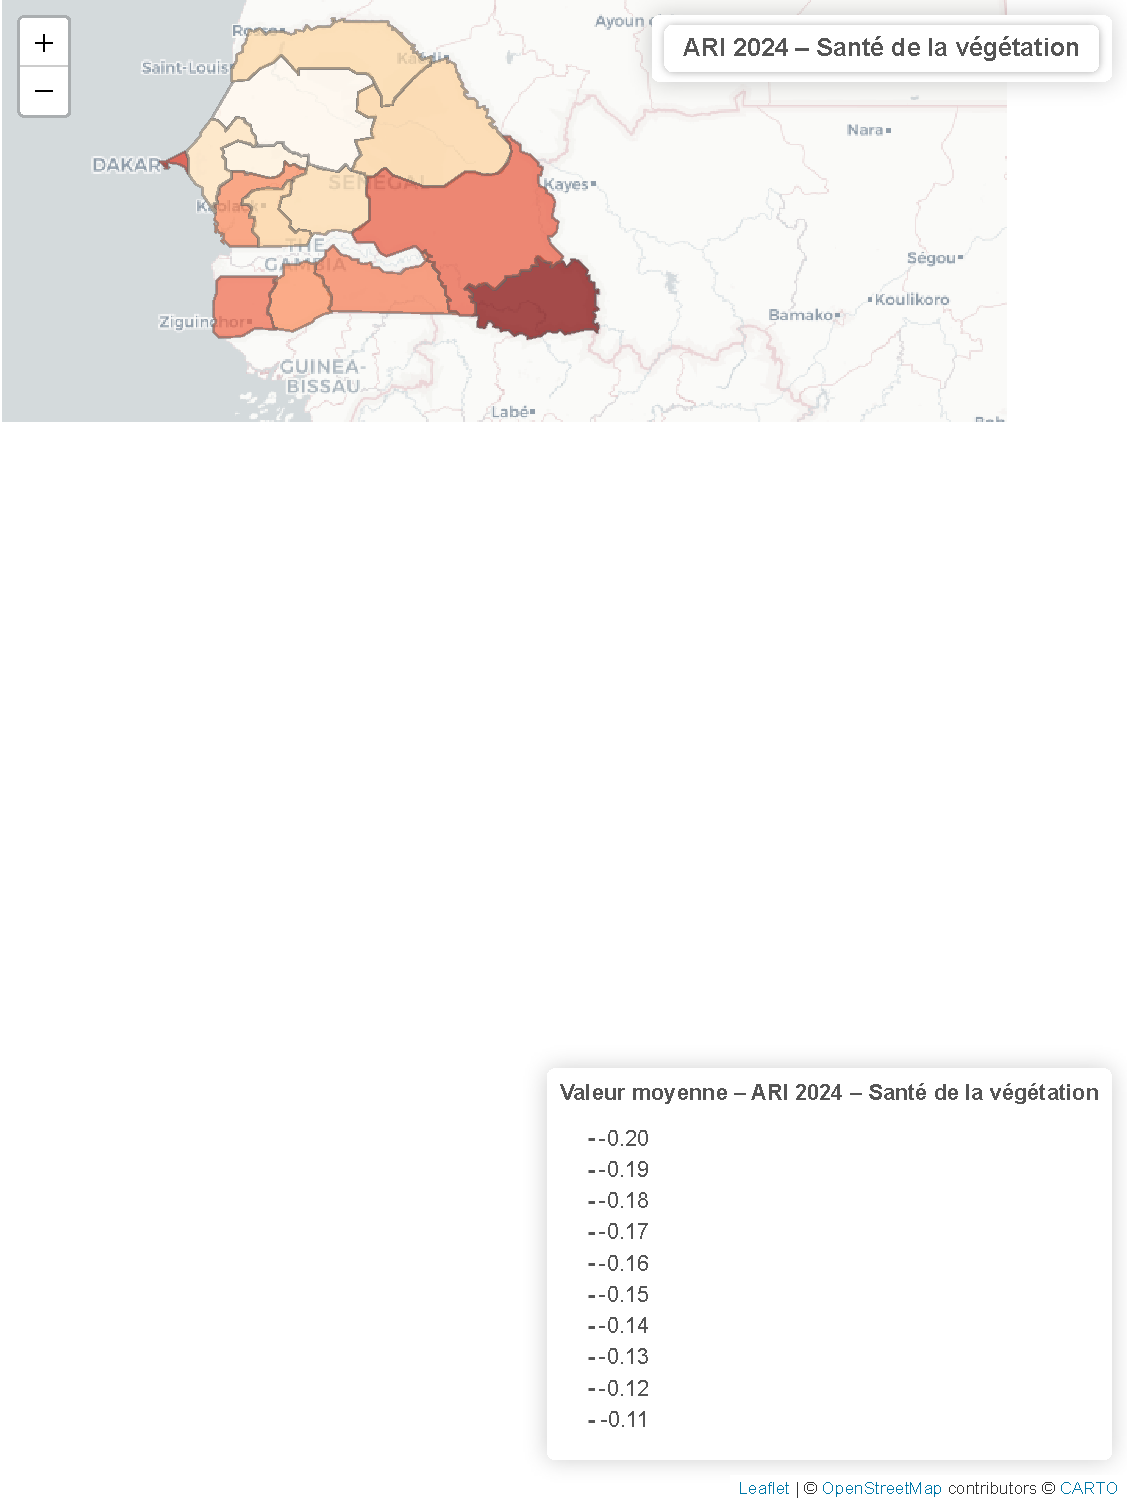
\includegraphics{Atlas-Spectral-Sahel_files/figure-latex/vegetation-ari-1.pdf}

\subsection{Tableau de la répartition de l'ARI au Sénégal en 2024}\label{tableau-de-la-ruxe9partition-de-lari-au-suxe9nuxe9gal-en-2024}

\begin{table}[!t]
\caption*{
{\large ** Moyennes régionales de l'ARI **} \\ 
{\small \emph{Sénégal -- Année 2024}}
} 
\fontsize{12.0pt}{14.4pt}\selectfont
\begin{tabular*}{\linewidth}{@{\extracolsep{\fill}}lr}
\toprule
{RÉGION} & {ARI} \\ 
\midrule\addlinespace[2.5pt]
Dakar & {\cellcolor[HTML]{C6171C}{\textcolor[HTML]{FFFFFF}{-0.130}}} \\ 
Diourbel & {\cellcolor[HTML]{FFECE3}{\textcolor[HTML]{000000}{-0.199}}} \\ 
Fatick & {\cellcolor[HTML]{F96244}{\textcolor[HTML]{FFFFFF}{-0.153}}} \\ 
Kaffrine & {\cellcolor[HTML]{FDC3AB}{\textcolor[HTML]{000000}{-0.183}}} \\ 
Kaolack & {\cellcolor[HTML]{FCB499}{\textcolor[HTML]{000000}{-0.178}}} \\ 
Kédougou & {\cellcolor[HTML]{67000D}{\textcolor[HTML]{FFFFFF}{-0.107}}} \\ 
Kolda & {\cellcolor[HTML]{F55239}{\textcolor[HTML]{FFFFFF}{-0.149}}} \\ 
Louga & {\cellcolor[HTML]{FFF5F0}{\textcolor[HTML]{000000}{-0.205}}} \\ 
Matam & {\cellcolor[HTML]{FCB59A}{\textcolor[HTML]{000000}{-0.179}}} \\ 
Saint-Louis & {\cellcolor[HTML]{FCBEA5}{\textcolor[HTML]{000000}{-0.181}}} \\ 
Sédhiou & {\cellcolor[HTML]{FA6748}{\textcolor[HTML]{FFFFFF}{-0.155}}} \\ 
Tambacounda & {\cellcolor[HTML]{E33127}{\textcolor[HTML]{FFFFFF}{-0.140}}} \\ 
Thiès & {\cellcolor[HTML]{FED2C0}{\textcolor[HTML]{000000}{-0.188}}} \\ 
Ziguinchor & {\cellcolor[HTML]{EF3C2C}{\textcolor[HTML]{FFFFFF}{-0.144}}} \\ 
\bottomrule
\end{tabular*}
\end{table}

\subsection{Analyse des résultats}\label{analyse-des-ruxe9sultats-1}

L'ARI permet d'identifier les zones où la végétation est soumise à des stress environnementaux (sécheresse, pollution, maladies, etc.). Il complète ainsi le NDVI en fournissant une information sur la qualité de la végétation, au-delà de sa seule quantité.

On observe d'abord un \textbf{stress végétal} marqué dans les régions où l'ARI dépasse \textbf{--0.15}, indiquant une concentration élevée d'anthocyanines. Ces pigments sont souvent révélateurs d'un stress physiologique important chez les plantes. C'est le cas de \textbf{Kédougou (--0.1069)}, qui apparaît comme la région la plus touchée. Cela peut s'expliquer par la présence de forêts secondaires en dégradation ou encore par une végétation soumise à des pressions liées à l'agriculture minière ou de subsistance. \textbf{Dakar (--0.1297)} présente également un niveau élevé de stress, probablement en lien avec la végétation urbaine soumise à un stress hydrique chronique. Les cas de \textbf{Tambacounda (--0.1397)} et \textbf{Ziguinchor (--0.1438)} peuvent sembler paradoxaux, car ce sont des zones théoriquement bien végétalisées. Pourtant, cela suggère que la végétation dense dans ces zones subit un stress réel, possiblement lié à la déforestation, aux variations hydriques saisonnières ou à une intensification agricole.

Un \textbf{stress modéré}, avec des valeurs d'ARI comprises entre \textbf{--0.15 et --0.18}, est observé dans des régions comme \textbf{Sédhiou, Kolda et Fatick}. Ces zones agricoles ou forestières en transition présentent une végétation active mais déjà soumise à certaines pressions, comme la saison sèche ou la pression anthropique. De leur côté, \textbf{Kaolack et Matam} affichent également des valeurs intermédiaires, avec des situations contrastées : Kaolack est marquée par une végétation saisonnière influencée par la régularité des pluies, tandis que Matam, plus sahélienne, possède une végétation clairsemée mais relativement stable.

Enfin, certaines régions présentent des valeurs \textbf{très faibles} de l'ARI, proches de \textbf{--0.20,} comme \textbf{Diourbel, Kaffrine et Louga}. Ces régions, situées dans des zones semi-arides ou sahéliennes, ne doivent pas être interprétées hâtivement comme bénéficiant d'une bonne santé végétale. En réalité, leur faible score ARI s'explique par une couverture végétale très réduite. Moins il y a de végétation, moins il y a de pigments à détecter, ce qui entraîne mécaniquement un indice faible. Cela traduit davantage une absence de végétation mesurable qu'un véritable état de santé écologique favorable.

\begin{center}\rule{0.5\linewidth}{0.5pt}\end{center}

\section{Eau et humidité -- LSWI}\label{eau-et-humidituxe9-lswi}

Le LSWI (Land Surface Water Index) est un indice spectral conçu pour détecter la présence d'humidité dans la végétation et dans le sol. Il est sensible à l'eau contenue dans les feuilles et à la teneur en eau des surfaces, ce qui en fait un indicateur précieux pour évaluer les conditions hydriques des écosystèmes. Le LSWI est particulièrement utile dans les zones agricoles et humides, car il permet de suivre les variations saisonnières de l'humidité des sols et des plantes.

Contrairement au NDVI, qui met l'accent sur la densité du couvert végétal, ou à l'ARI qui explore les stress biochimiques internes, le LSWI renseigne directement sur l'état hydrique du couvert terrestre.

Dans le cas du Sénégal, les valeurs moyennes du LSWI pour l'année 2024 ont été extraites à partir de rasters satellitaires à haute résolution, puis agrégées par région administrative.

\subsection{Carte interactive du LSWI au Sénégal en 2024}\label{carte-interactive-du-lswi-au-suxe9nuxe9gal-en-2024}

\begin{verbatim}
##   |                                                                              |                                                                      |   0%  |                                                                              |=====                                                                 |   7%  |                                                                              |==========                                                            |  14%  |                                                                              |===============                                                       |  21%  |                                                                              |====================                                                  |  29%  |                                                                              |=========================                                             |  36%  |                                                                              |==============================                                        |  43%  |                                                                              |===================================                                   |  50%  |                                                                              |========================================                              |  57%  |                                                                              |=============================================                         |  64%  |                                                                              |==================================================                    |  71%  |                                                                              |=======================================================               |  79%  |                                                                              |============================================================          |  86%  |                                                                              |=================================================================     |  93%  |                                                                              |======================================================================| 100%
\end{verbatim}

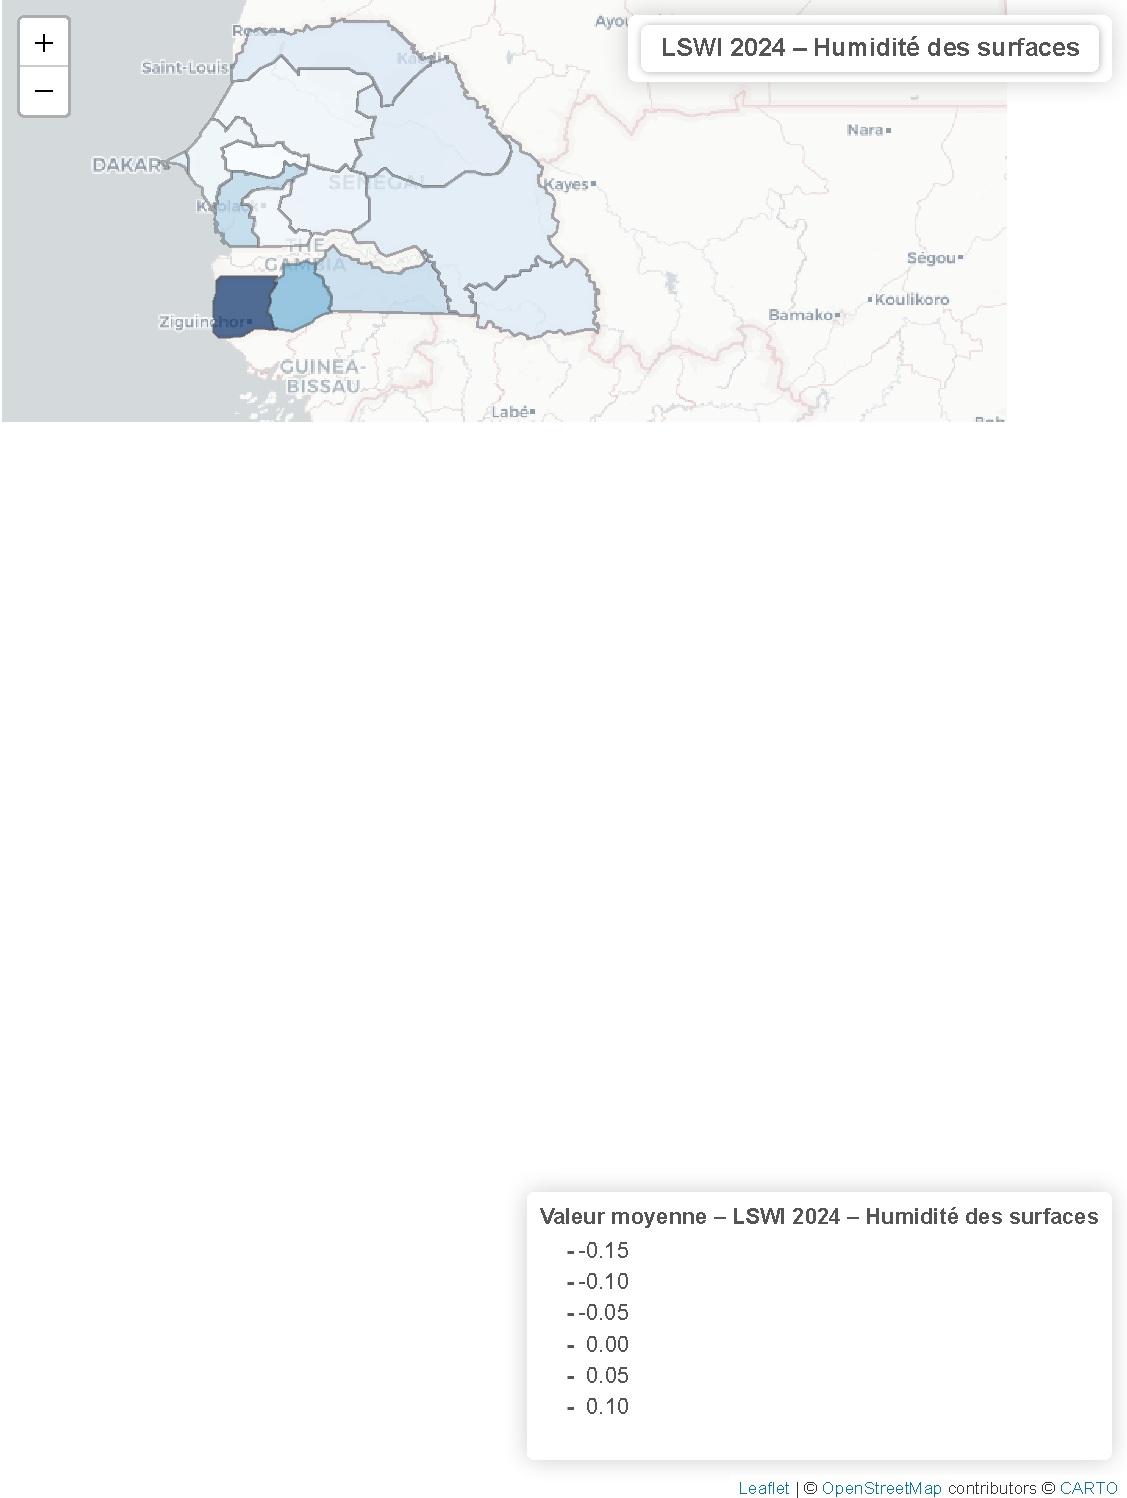
\includegraphics{Atlas-Spectral-Sahel_files/figure-latex/eau-lswi-1.pdf}

\subsection{Tableau de la répartition du LSWI au Sénégal en 2024}\label{tableau-de-la-ruxe9partition-du-lswi-au-suxe9nuxe9gal-en-2024}

\begin{table}[!t]
\caption*{
{\large \textbf{Moyennes régionales du LSWI}} \\ 
{\small \emph{Sénégal -- Année 2024}}
} 
\fontsize{12.0pt}{14.4pt}\selectfont
\begin{tabular*}{\linewidth}{@{\extracolsep{\fill}}lr}
\toprule
{RÉGION} & {LSWI} \\ 
\midrule\addlinespace[2.5pt]
Dakar & {\cellcolor[HTML]{DCEAF6}{\textcolor[HTML]{000000}{-0.118}}} \\ 
Diourbel & {\cellcolor[HTML]{F7FBFF}{\textcolor[HTML]{000000}{-0.157}}} \\ 
Fatick & {\cellcolor[HTML]{B2D2E8}{\textcolor[HTML]{000000}{-0.065}}} \\ 
Kaffrine & {\cellcolor[HTML]{E6F0F9}{\textcolor[HTML]{000000}{-0.132}}} \\ 
Kaolack & {\cellcolor[HTML]{EFF6FC}{\textcolor[HTML]{000000}{-0.145}}} \\ 
Kédougou & {\cellcolor[HTML]{DBE9F6}{\textcolor[HTML]{000000}{-0.116}}} \\ 
Kolda & {\cellcolor[HTML]{BBD6EB}{\textcolor[HTML]{000000}{-0.074}}} \\ 
Louga & {\cellcolor[HTML]{EDF5FC}{\textcolor[HTML]{000000}{-0.142}}} \\ 
Matam & {\cellcolor[HTML]{DCE9F6}{\textcolor[HTML]{000000}{-0.117}}} \\ 
Saint-Louis & {\cellcolor[HTML]{D7E6F5}{\textcolor[HTML]{000000}{-0.110}}} \\ 
Sédhiou & {\cellcolor[HTML]{6EAFD7}{\textcolor[HTML]{000000}{-0.013}}} \\ 
Tambacounda & {\cellcolor[HTML]{DAE8F6}{\textcolor[HTML]{000000}{-0.115}}} \\ 
Thiès & {\cellcolor[HTML]{EBF3FB}{\textcolor[HTML]{000000}{-0.140}}} \\ 
Ziguinchor & {\cellcolor[HTML]{08306B}{\textcolor[HTML]{FFFFFF}{0.135}}} \\ 
\bottomrule
\end{tabular*}
\end{table}

\subsection{Analyse des résultats}\label{analyse-des-ruxe9sultats-2}

Les résultats montrent une variabilité spatiale importante entre le sud tropical humide et le nord sahélien du Sénégal.

\textbf{Régions à forte humidité (LSWI \textgreater{} 0)}

La seule région présentant une valeur positive est \textbf{Ziguinchor (0.1354)}, ce qui traduit une très forte teneur en eau dans les surfaces végétalisées et les sols. Cette valeur confirme le caractère très humide de la région, qui bénéficie de précipitations abondantes, d'un couvert forestier dense et de nombreuses zones humides (bolongs, forêts galeries, rizières). Elle représente la zone la plus hydratée du pays selon cet indice.

\textbf{Régions modérément humides (LSWI entre --0.05 et --0.1)}

\textbf{Sédhiou (--0.0127)} et \textbf{Kolda (--0.0737)} affichent également des niveaux élevés d'humidité relative, bien que les valeurs soient légèrement négatives. Cela traduit un environnement encore bien alimenté en eau, probablement en saison humide, avec une végétation active et des sols encore hydratés.

\textbf{Fatick (--0.0651)} suit cette tendance, en lien avec la présence de zones de mangrove et de marigots dans le Sine-Saloum.

Ces régions constituent donc un socle écologique important, où l'accès à l'eau reste favorable à l'agriculture et à la biodiversité.

\textbf{Régions de transition hydrique} \textbf{(LSWI entre --0.10 et --0.13)}

On retrouve ici \textbf{Kédougou (--0.1155)}, \textbf{Tambacounda (--0.1146)}, \textbf{Saint-Louis (--0.1099)}, \textbf{Matam (--0.1171)} et \textbf{Dakar (--0.1178)}.

Ce sont des régions qui subissent des variations hydriques saisonnières importantes, voire des contrastes locaux (zones humides vs.~sèches).

À Saint-Louis ou Matam, la proximité du fleuve Sénégal peut créer des poches d'humidité malgré un environnement plus aride.

À Dakar, l'urbanisation limite la rétention d'eau, mais certains espaces verts et zones côtières conservent une humidité relative.

\textbf{Régions les plus sèches (LSWI \textless{} --0.13)}

\textbf{Kaolack (--0.1449)}, \textbf{Thiès (--0.1400)}, \textbf{Louga (--0.1425)}, \textbf{Diourbel (--0.1572)} et \textbf{Kaffrine (--0.1319)} enregistrent les valeurs LSWI les plus basses.

Cela traduit une faible humidité des sols et de la végétation, cohérente avec des précipitations faibles, une végétation discontinue, et un stress hydrique plus marqué.

\section{Conclusion}\label{conclusion}

L'analyse des dynamiques environnementales du Sénégal en 2024 à travers les indices spectraux NDVI, ARI et LSWI met en évidence des contrastes écologiques marqués entre les régions, révélateurs d'un gradient climatique, végétal et hydrique du nord au sud.

L'indice NDVI montre une densité de végétation élevée dans les régions méridionales telles que Ziguinchor, Kolda et Sédhiou, reflet de conditions agro-écologiques favorables. À l'inverse, les régions sahéliennes du nord comme Matam, Louga ou Saint-Louis affichent des valeurs nettement plus faibles, traduisant une couverture végétale clairsemée et des sols plus dégradés.

L'ARI, indicateur de stress végétal, complète cette lecture en soulignant que certaines zones pourtant verdoyantes (ex. Kédougou, Ziguinchor, Tambacounda) présentent une végétation soumise à un stress biochimique non négligeable, probablement lié à l'intensification agricole, aux pressions anthropiques ou à la variabilité climatique. À l'inverse, des régions arides affichent un ARI faible, non pas par bonne santé, mais en raison de la rareté de végétation détectable.

Enfin, l'indice LSWI permet d'évaluer la teneur en eau des surfaces et des végétaux. Il révèle une forte humidité dans les zones tropicales du sud (notamment Ziguinchor et Sédhiou), des niveaux intermédiaires dans les zones de transition (Kolda, Fatick), et une situation de déficit hydrique croissant en remontant vers le nord.

En somme, ce chapitre offre une lecture écologique intégrée du territoire sénégalais, où chaque indice apporte un éclairage complémentaire : le NDVI mesure la quantité de végétation, l'ARI en évalue la santé, et le LSWI renseigne sur l'humidité disponible. Leur croisement permet d'identifier les zones de résilience écologique, mais aussi les régions vulnérables aux dégradations, appelant à des actions de gestion ciblées. Ces résultats serviront de base pour les comparaisons inter-pays présentées dans les chapitres suivants.

\begin{quote}
\emph{``Chaque pixel est une parcelle d'histoire écologique. Ensemble, ils dessinent la carte du vivant.''}
\end{quote}

\chapter{Burkina}\label{burkina}

\section{Introduction}\label{introduction-1}

Le \textbf{Burkina Faso}, situé au cœur du \textbf{Sahel}, est un territoire à la fois stratégique et fragile sur le plan écologique. Son environnement est caractérisé par une transition marquée entre les zones arides du nord, soumises à la désertification, et les régions sud-soudaniennes plus humides et agricoles. Cette diversité spatiale, combinée à une forte pression démographique et à des aléas climatiques récurrents, fait du Burkina Faso un terrain d'étude privilégié pour analyser les dynamiques environnementales en contexte sahélien.

Dans ce chapitre, trois indices spectraux issus d'images satellitaires sont mobilisés pour caractériser l'état écologique du Burkina Faso en 2024, chacun apportant un éclairage complémentaire :

Le \textbf{BNDVI (Blue Normalized Difference Vegetation Index)} permet d'évaluer la couverture végétale en intégrant la bande bleue du spectre, ce qui en fait un indice particulièrement sensible dans les zones à faible végétation --- typiques des régions sahéliennes ;

Le \textbf{BAI (Burned Area Index)} est ici utilisé comme un indicateur de stress extrême ou de dégradation écologique, notamment en lien avec les feux de brousse, la sécheresse ou la surexploitation des sols ;

Le \textbf{AWEInsh (Automated Water Extraction Index -- non-shaded)} détecte la présence d'humidité dans les sols et la végétation, un facteur clé dans un pays où l'accès à l'eau reste un enjeu environnemental et socio-économique majeur.

Ces indices sont analysés à l'échelle régionale, à travers des cartes interactives, des tableaux statistiques et des commentaires interprétatifs. Cette approche permet de repérer les zones écologiquement stables, d'identifier les régions sous stress ou à risque de dégradation, et de proposer des lectures spatialisées de la vulnérabilité environnementale.

Ce chapitre constitue ainsi une lecture écologique intégrée du Burkina Faso, en apportant une vision à la fois descriptive et analytique des conditions végétales, hydriques et dégradatives du territoire, dans une logique de comparaison avec les autres pays de l'Atlas.

\begin{center}\rule{0.5\linewidth}{0.5pt}\end{center}

\section{Végétation -- BNDVI}\label{vuxe9guxe9tation-bndvi}

Le \textbf{BNDVI (Blue Normalized Difference Vegetation Index)} est une variante du NDVI qui utilise la bande bleue au lieu de la bande rouge dans son calcul. Il permet de mesurer la densité et la vigueur de la végétation verte, en particulier dans les zones à faible couverture végétale ou soumises à des effets atmosphériques importants comme les aérosols ou la poussière, fréquents dans les environnements sahéliens.

Ses valeurs sont généralement comprises entre \textbf{--1} et \textbf{+1}, mais dans les milieux naturels, elles se situent plutôt entre \textbf{0 (sol nu ou zones dégradées)} et \textbf{1 (végétation dense et active)}. En raison de la manière dont certains rasters sont enregistrés, les valeurs sont parfois multipliées par 10 000, ce qui est corrigé dans notre analyse.

Dans le cas du Burkina Faso, nous avons extrait les valeurs moyennes du BNDVI pour l'année 2024 par région administrative, à partir de rasters satellitaires haute résolution. Ces valeurs permettent de dresser une cartographie précise de la répartition de la végétation sur le territoire, et de mettre en évidence les contrastes écologiques entre les régions du nord, plus arides, et celles du sud, plus verdoyantes.

\subsection{Carte interactive du BNDVI au Burkina-Faso en 2024}\label{carte-interactive-du-bndvi-au-burkina-faso-en-2024}

\begin{verbatim}
##   |                                                                              |                                                                      |   0%  |                                                                              |=====                                                                 |   8%  |                                                                              |===========                                                           |  15%  |                                                                              |================                                                      |  23%  |                                                                              |======================                                                |  31%  |                                                                              |===========================                                           |  38%  |                                                                              |================================                                      |  46%  |                                                                              |======================================                                |  54%  |                                                                              |===========================================                           |  62%  |                                                                              |================================================                      |  69%  |                                                                              |======================================================                |  77%  |                                                                              |===========================================================           |  85%  |                                                                              |=================================================================     |  92%  |                                                                              |======================================================================| 100%
\end{verbatim}

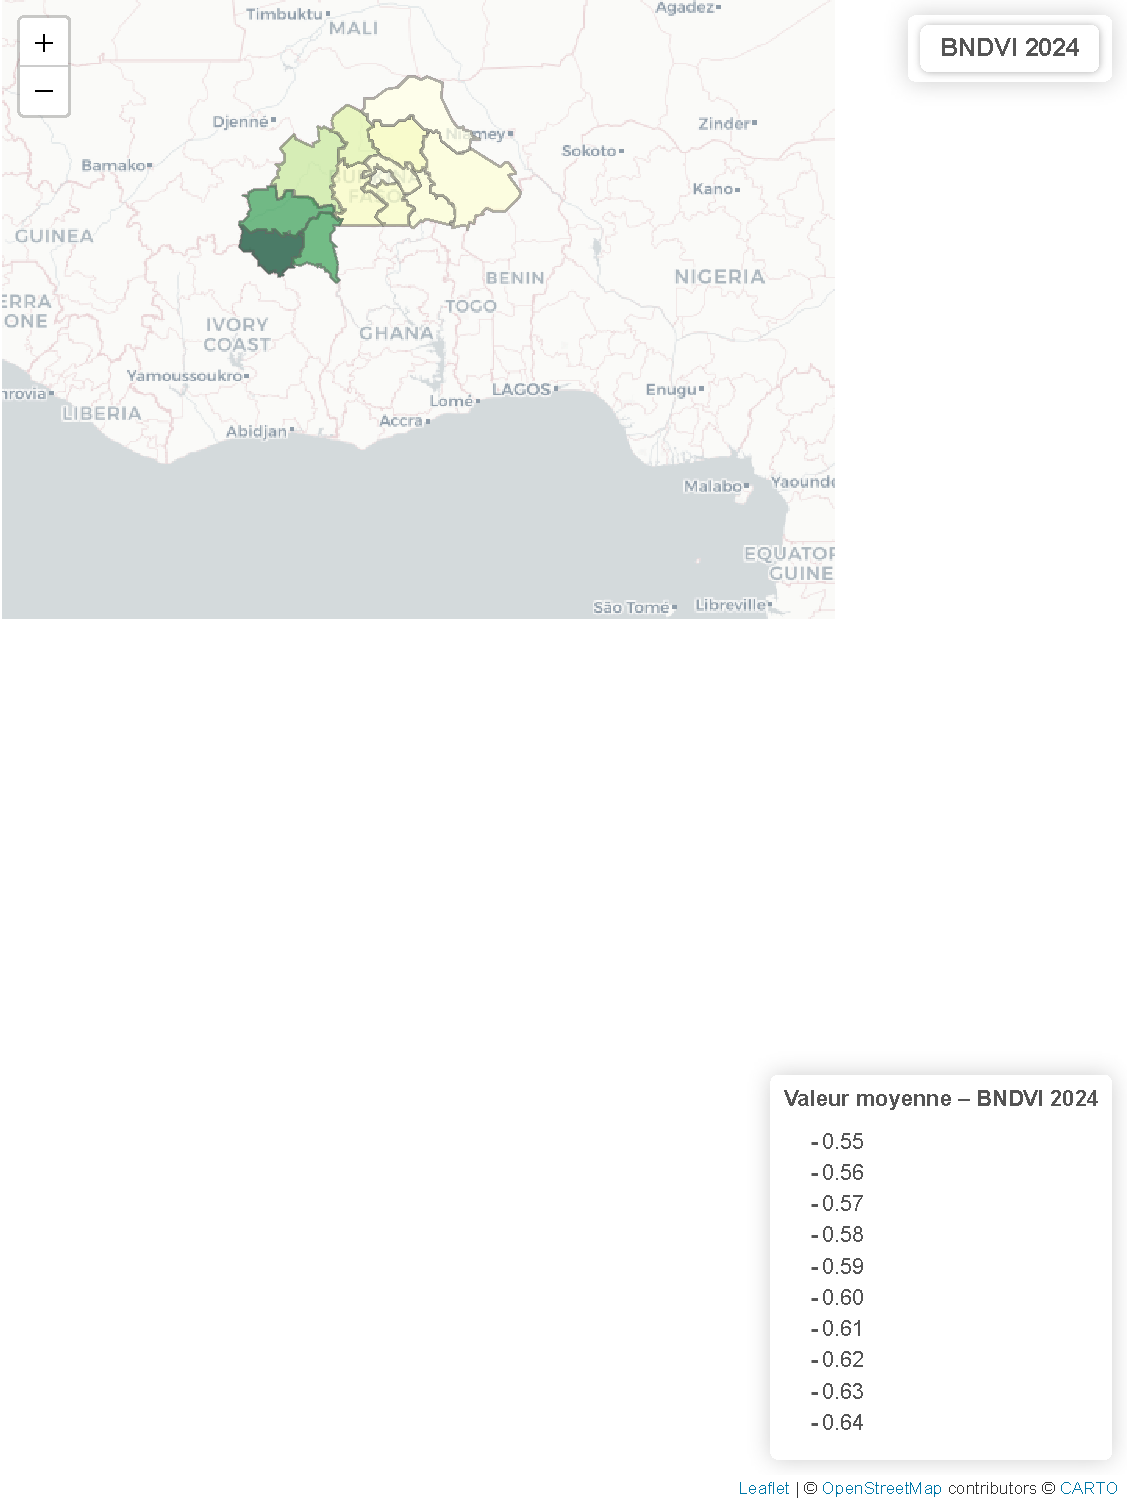
\includegraphics{Atlas-Spectral-Sahel_files/figure-latex/vegetation-bndvi-1.pdf}

\subsection{Tableau de la répartition du BNDVI au Burkina en 2024}\label{tableau-de-la-ruxe9partition-du-bndvi-au-burkina-en-2024}

\begin{table}[!t]
\caption*{
{\large \textbf{Moyennes régionales du BNDVI}} \\ 
{\small \emph{Burkina-Faso -- Année 2024}}
} 
\fontsize{12.0pt}{14.4pt}\selectfont
\begin{tabular*}{\linewidth}{@{\extracolsep{\fill}}lr}
\toprule
{RÉGION} & {BNDVI} \\ 
\midrule\addlinespace[2.5pt]
Boucle du Mouhoun & {\cellcolor[HTML]{C7E89A}{\textcolor[HTML]{000000}{0.57}}} \\ 
Cascades & {\cellcolor[HTML]{004529}{\textcolor[HTML]{FFFFFF}{0.64}}} \\ 
Centre & {\cellcolor[HTML]{FEFFE1}{\textcolor[HTML]{000000}{0.55}}} \\ 
Centre-Est & {\cellcolor[HTML]{FCFED3}{\textcolor[HTML]{000000}{0.55}}} \\ 
Centre-Nord & {\cellcolor[HTML]{F7FCB9}{\textcolor[HTML]{000000}{0.56}}} \\ 
Centre-Ouest & {\cellcolor[HTML]{F9FCC0}{\textcolor[HTML]{000000}{0.56}}} \\ 
Centre-Sud & {\cellcolor[HTML]{F9FDC4}{\textcolor[HTML]{000000}{0.56}}} \\ 
Est & {\cellcolor[HTML]{FDFED6}{\textcolor[HTML]{000000}{0.55}}} \\ 
Hauts-Bassins & {\cellcolor[HTML]{379E54}{\textcolor[HTML]{FFFFFF}{0.61}}} \\ 
Nord & {\cellcolor[HTML]{E1F3A8}{\textcolor[HTML]{000000}{0.57}}} \\ 
Plateau-Central & {\cellcolor[HTML]{FBFDCF}{\textcolor[HTML]{000000}{0.55}}} \\ 
Sahel & {\cellcolor[HTML]{FFFFE5}{\textcolor[HTML]{000000}{0.55}}} \\ 
Sud-Ouest & {\cellcolor[HTML]{3AA156}{\textcolor[HTML]{FFFFFF}{0.61}}} \\ 
\bottomrule
\end{tabular*}
\end{table}

\subsection{Analyse des résultats}\label{analyse-des-ruxe9sultats-3}

L'analyse zonale du \textbf{BNDVI} permet de :

\begin{itemize}
\tightlist
\item
  Quantifier la \textbf{productivité végétale régionale} dans un contexte sahélien soumis à de fortes pressions climatiques,
\item
  Détecter les \textbf{zones à faible couverture végétale}, potentiellement exposées à la désertification et à l'érosion des sols,
\item
  Orienter les \textbf{politiques agricoles, forestières et pastorales} en tenant compte des disparités régionales,
\item
  Comparer les \textbf{dynamiques écologiques} entre le nord aride, les savanes centrales et les zones soudaniennes du sud-ouest.
\end{itemize}

La répartition régionale du BNDVI au \textbf{Burkina Faso en 2024} révèle une \textbf{variabilité modérée} de la couverture végétale, avec des valeurs comprises entre \textbf{0.55 et 0.64}, mais elle met en évidence un \textbf{gradient écologique sud-ouest / nord-est}.

Les \textbf{valeurs les plus élevées}, supérieures à \textbf{0.60}, sont enregistrées dans les régions du \textbf{Sud-Ouest (0.61)}, des \textbf{Hauts-Bassins (0.61)} et des \textbf{Cascades (0.64)}. Ces zones bénéficient d'une \textbf{pluviométrie plus abondante}, d'un \textbf{sol plus fertile}, et d'une \textbf{densité forestière plus importante}. Elles concentrent également une part importante de la production agricole nationale.

Les \textbf{valeurs intermédiaires}, autour de \textbf{0.56 à 0.57}, sont observées dans des régions de transition comme la \textbf{Boucle du Mouhoun}, le \textbf{Nord}, le \textbf{Centre-Ouest}, ou encore le \textbf{Centre-Nord}. Ces zones présentent généralement une \textbf{végétation saisonnière}, composée de savanes, de jachères et de zones cultivées.

Les \textbf{valeurs les plus faibles} du BNDVI, bien qu'elles restent relativement élevées (autour de \textbf{0.55}), sont relevées dans des régions plus arides ou urbanisées telles que le \textbf{Plateau-Central}, le \textbf{Centre}, l'\textbf{Est}, et la région sahélienne du \textbf{Sahel}. Dans ces territoires, la couverture végétale est \textbf{plus clairsemée}, souvent soumise à un \textbf{stress hydrique chronique}, à une \textbf{déforestation progressive}, ou à une \textbf{occupation du sol plus anthropisée}.

Globalement, cette carte illustre une \textbf{transition écologique ouest-sud / nord-est} caractéristique du Burkina Faso : les zones méridionales et occidentales concentrent la \textbf{végétation la plus dense et active}, tandis que les régions du centre et du nord, plus exposées aux aléas climatiques et à la pression démographique, affichent une \textbf{couverture végétale plus fragile}.

\begin{center}\rule{0.5\linewidth}{0.5pt}\end{center}

\section{Santé de la végétation -- BAI}\label{santuxe9-de-la-vuxe9guxe9tation-bai}

Le \textbf{BAI (Burned Area Index)} est un indice spectral développé à l'origine pour \textbf{détecter les zones brûlées} par les incendies de végétation. Toutefois, dans les contextes sahéliens comme celui du \textbf{Burkina Faso}, le BAI est également utilisé comme un \textbf{indicateur de stress ou de dégradation avancée}, car il met en évidence des sols nus, sombres, souvent liés à une \textbf{perte de couvert végétal}, à la \textbf{sécheresse}, ou à une \textbf{surexploitation agricole et pastorale}.

Le BAI est calculé à partir des bandes \textbf{rouge} et \textbf{infrarouge moyen (SWIR)}, avec une sensibilité particulière aux zones où la végétation a disparu ou subi une altération profonde. Contrairement aux indices comme le NDVI ou le BNDVI, qui mesurent la densité de la végétation, le BAI met plutôt en évidence les \textbf{signes visibles de perturbation ou d'appauvrissement de la surface terrestre}.

Dans le cas du \textbf{Burkina Faso}, nous avons extrait les \textbf{valeurs moyennes du BAI pour l'année 2024} à partir d'images satellites haute résolution, puis agrégé ces résultats \textbf{par région administrative}. L'analyse permet d'identifier les zones \textbf{écologiquement les plus fragilisées}, où les pressions climatiques et anthropiques ont laissé des traces visibles dans la structure du sol et du couvert végétal.

\subsection{Carte interactive du BAI au Burkina-Faso en 2024}\label{carte-interactive-du-bai-au-burkina-faso-en-2024}

\begin{verbatim}
##   |                                                                              |                                                                      |   0%  |                                                                              |=====                                                                 |   8%  |                                                                              |===========                                                           |  15%  |                                                                              |================                                                      |  23%  |                                                                              |======================                                                |  31%  |                                                                              |===========================                                           |  38%  |                                                                              |================================                                      |  46%  |                                                                              |======================================                                |  54%  |                                                                              |===========================================                           |  62%  |                                                                              |================================================                      |  69%  |                                                                              |======================================================                |  77%  |                                                                              |===========================================================           |  85%  |                                                                              |=================================================================     |  92%  |                                                                              |======================================================================| 100%
\end{verbatim}

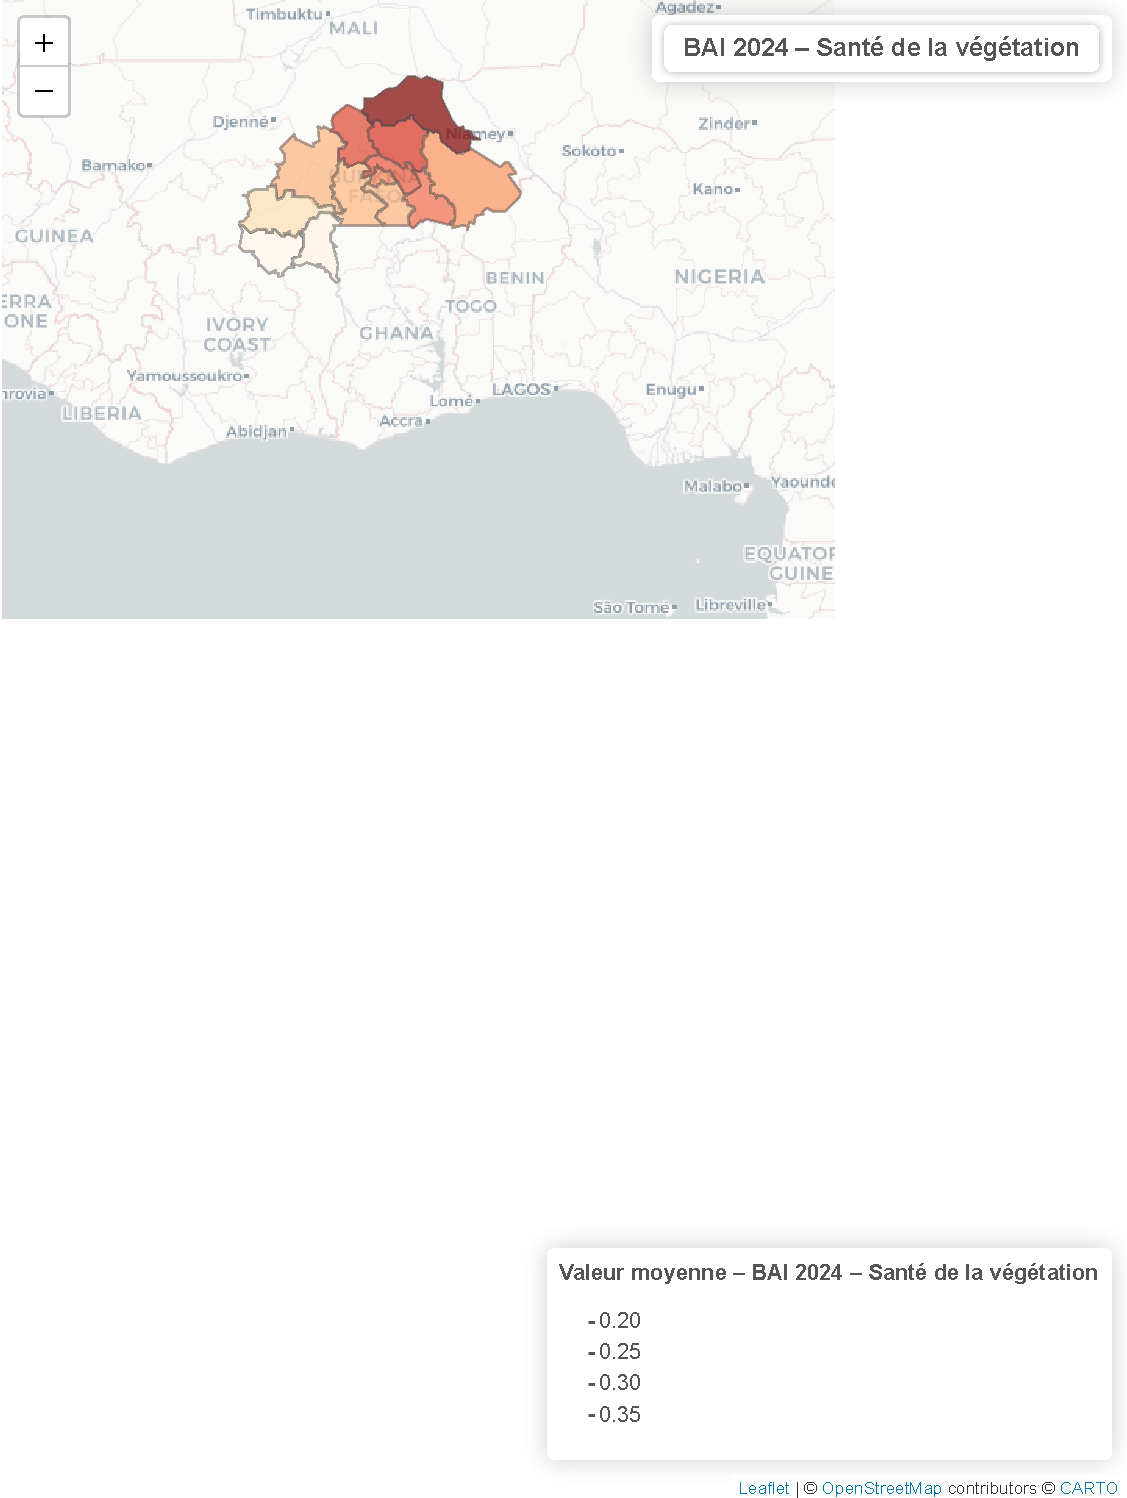
\includegraphics{Atlas-Spectral-Sahel_files/figure-latex/vegetation-bai-1.pdf}

\subsection{Tableau de la répartition du BAI au Burkina en 2024}\label{tableau-de-la-ruxe9partition-du-bai-au-burkina-en-2024}

\begin{table}[!t]
\caption*{
{\large \textbf{Moyennes régionales du BAI}} \\ 
{\small \emph{Burkina-Faso -- Année 2024}}
} 
\fontsize{12.0pt}{14.4pt}\selectfont
\begin{tabular*}{\linewidth}{@{\extracolsep{\fill}}lr}
\toprule
{RÉGION} & {BAI} \\ 
\midrule\addlinespace[2.5pt]
Boucle du Mouhoun & {\cellcolor[HTML]{FC8B6B}{\textcolor[HTML]{000000}{0.25}}} \\ 
Cascades & {\cellcolor[HTML]{FFF5F0}{\textcolor[HTML]{000000}{0.17}}} \\ 
Centre & {\cellcolor[HTML]{F75A3F}{\textcolor[HTML]{FFFFFF}{0.28}}} \\ 
Centre-Est & {\cellcolor[HTML]{F14230}{\textcolor[HTML]{FFFFFF}{0.29}}} \\ 
Centre-Nord & {\cellcolor[HTML]{CB181D}{\textcolor[HTML]{FFFFFF}{0.32}}} \\ 
Centre-Ouest & {\cellcolor[HTML]{FC8E6E}{\textcolor[HTML]{000000}{0.25}}} \\ 
Centre-Sud & {\cellcolor[HTML]{FC8C6B}{\textcolor[HTML]{000000}{0.25}}} \\ 
Est & {\cellcolor[HTML]{FB6E4E}{\textcolor[HTML]{FFFFFF}{0.27}}} \\ 
Hauts-Bassins & {\cellcolor[HTML]{FECEB9}{\textcolor[HTML]{000000}{0.21}}} \\ 
Nord & {\cellcolor[HTML]{D92723}{\textcolor[HTML]{FFFFFF}{0.31}}} \\ 
Plateau-Central & {\cellcolor[HTML]{E63328}{\textcolor[HTML]{FFFFFF}{0.30}}} \\ 
Sahel & {\cellcolor[HTML]{67000D}{\textcolor[HTML]{FFFFFF}{0.37}}} \\ 
Sud-Ouest & {\cellcolor[HTML]{FFF0E8}{\textcolor[HTML]{000000}{0.18}}} \\ 
\bottomrule
\end{tabular*}
\end{table}

\subsection{Analyse des résultats}\label{analyse-des-ruxe9sultats-4}

L'analyse zonale du \textbf{BAI} permet de :

\begin{itemize}
\tightlist
\item
  Repérer les zones \textbf{écologiquement dégradées ou perturbées}, qu'il s'agisse de \textbf{surfaces brûlées}, de \textbf{sols nus}, ou de \textbf{végétation fortement altérée} ;
\item
  Détecter les \textbf{régions les plus sensibles} à la \textbf{déforestation, à la sécheresse}, ou à l'\textbf{érosion des terres} ;
\item
  Mieux comprendre l'impact cumulé des \textbf{activités humaines} (agriculture extensive, feux de brousse) et des \textbf{aléas climatiques} dans la dynamique environnementale du pays.
\end{itemize}

La répartition des valeurs du \textbf{BAI} au Burkina Faso en 2024 fait apparaître des contrastes significatifs entre les régions :

Les \textbf{valeurs les plus élevées} sont enregistrées dans les régions \textbf{sahéliennes et septentrionales}, notamment dans le \textbf{Sahel (0.37)}, le \textbf{Centre-Nord (0.32)}, le \textbf{Nord (0.31)} et le \textbf{Plateau-Central (0.30)}. Ces zones présentent des \textbf{signes marqués de dégradation} du couvert végétal, probablement liés à la \textbf{répétition des sécheresses}, aux \textbf{incendies de brousse}, et à une \textbf{pression humaine forte} sur les ressources naturelles. Elles constituent des \textbf{zones critiques de vulnérabilité écologique}.

Les \textbf{valeurs intermédiaires}, comprises entre \textbf{0.25 et 0.29}, concernent des régions comme le \textbf{Centre (0.28)}, l'\textbf{Est (0.27)}, ou le \textbf{Centre-Ouest (0.25)}. Ces territoires connaissent une \textbf{pression environnementale modérée}, où les surfaces altérées cohabitent avec des zones encore fonctionnelles sur le plan écologique.

Enfin, les \textbf{valeurs les plus faibles} du BAI, indicatives de \textbf{moindre perturbation}, sont observées dans les \textbf{régions méridionales et plus humides} : \textbf{Cascades (0.17)}, \textbf{Sud-Ouest (0.18)} et \textbf{Hauts-Bassins (0.21)}. Ces zones bénéficient d'une \textbf{pluviométrie plus régulière}, d'une \textbf{couverture végétale plus dense}, et d'une \textbf{moindre intensité des perturbations de surface} --- ce qui en fait des \textbf{réservoirs de résilience écologique} pour le pays.

Ainsi, la carte du BAI illustre une \textbf{dégradation croissante du nord au sud}, et permet de cibler les régions prioritaires pour des \textbf{actions de reforestation, de lutte contre l'érosion, ou de gestion durable des ressources}.

\begin{center}\rule{0.5\linewidth}{0.5pt}\end{center}

\section{Eau et humidité -- AWEInsh}\label{eau-et-humidituxe9-aweinsh}

Le \textbf{AWEInsh (Automated Water Extraction Index -- non-shaded)} est un indice spectral conçu pour détecter la \textbf{présence d'humidité et d'eau libre} à la surface du sol, en particulier dans les \textbf{zones non ombragées}. Il est particulièrement adapté aux environnements sahéliens où l'\textbf{eau est souvent peu visible}, diffuse ou en faible quantité. Le AWEInsh est largement utilisé pour \textbf{identifier les zones humides}, les \textbf{mares temporaires}, les \textbf{vallées inondables} ou encore la \textbf{teneur en eau résiduelle} dans les surfaces agricoles.

Contrairement au NDVI ou au BNDVI qui mesurent la densité du couvert végétal, et au BAI qui signale les zones dégradées, le AWEInsh renseigne directement sur la \textbf{disponibilité en eau à la surface} du territoire, qu'il s'agisse d'eau libre ou d'humidité stockée dans les premiers centimètres du sol.

Dans le cas du \textbf{Burkina Faso}, les \textbf{valeurs moyennes du AWEInsh pour l'année 2024} ont été extraites à partir de \textbf{rasters satellites à haute résolution}, puis \textbf{agrégées par région administrative}. L'analyse de ces données permet d'identifier les \textbf{zones à forte ou faible disponibilité en eau}, de suivre les \textbf{gradients d'humidité}, et d'anticiper les \textbf{zones à risque de stress hydrique} ou de \textbf{déficit agricole}. Cet indice est ainsi un outil stratégique pour le \textbf{suivi agro-hydrologique} dans un pays confronté à une vulnérabilité climatique croissante.

\subsection{Carte interactive de l'AWEInsh au Burkina-Faso en 2024}\label{carte-interactive-de-laweinsh-au-burkina-faso-en-2024}

\begin{verbatim}
##   |                                                                              |                                                                      |   0%  |                                                                              |=====                                                                 |   8%  |                                                                              |===========                                                           |  15%  |                                                                              |================                                                      |  23%  |                                                                              |======================                                                |  31%  |                                                                              |===========================                                           |  38%  |                                                                              |================================                                      |  46%  |                                                                              |======================================                                |  54%  |                                                                              |===========================================                           |  62%  |                                                                              |================================================                      |  69%  |                                                                              |======================================================                |  77%  |                                                                              |===========================================================           |  85%  |                                                                              |=================================================================     |  92%  |                                                                              |======================================================================| 100%
\end{verbatim}

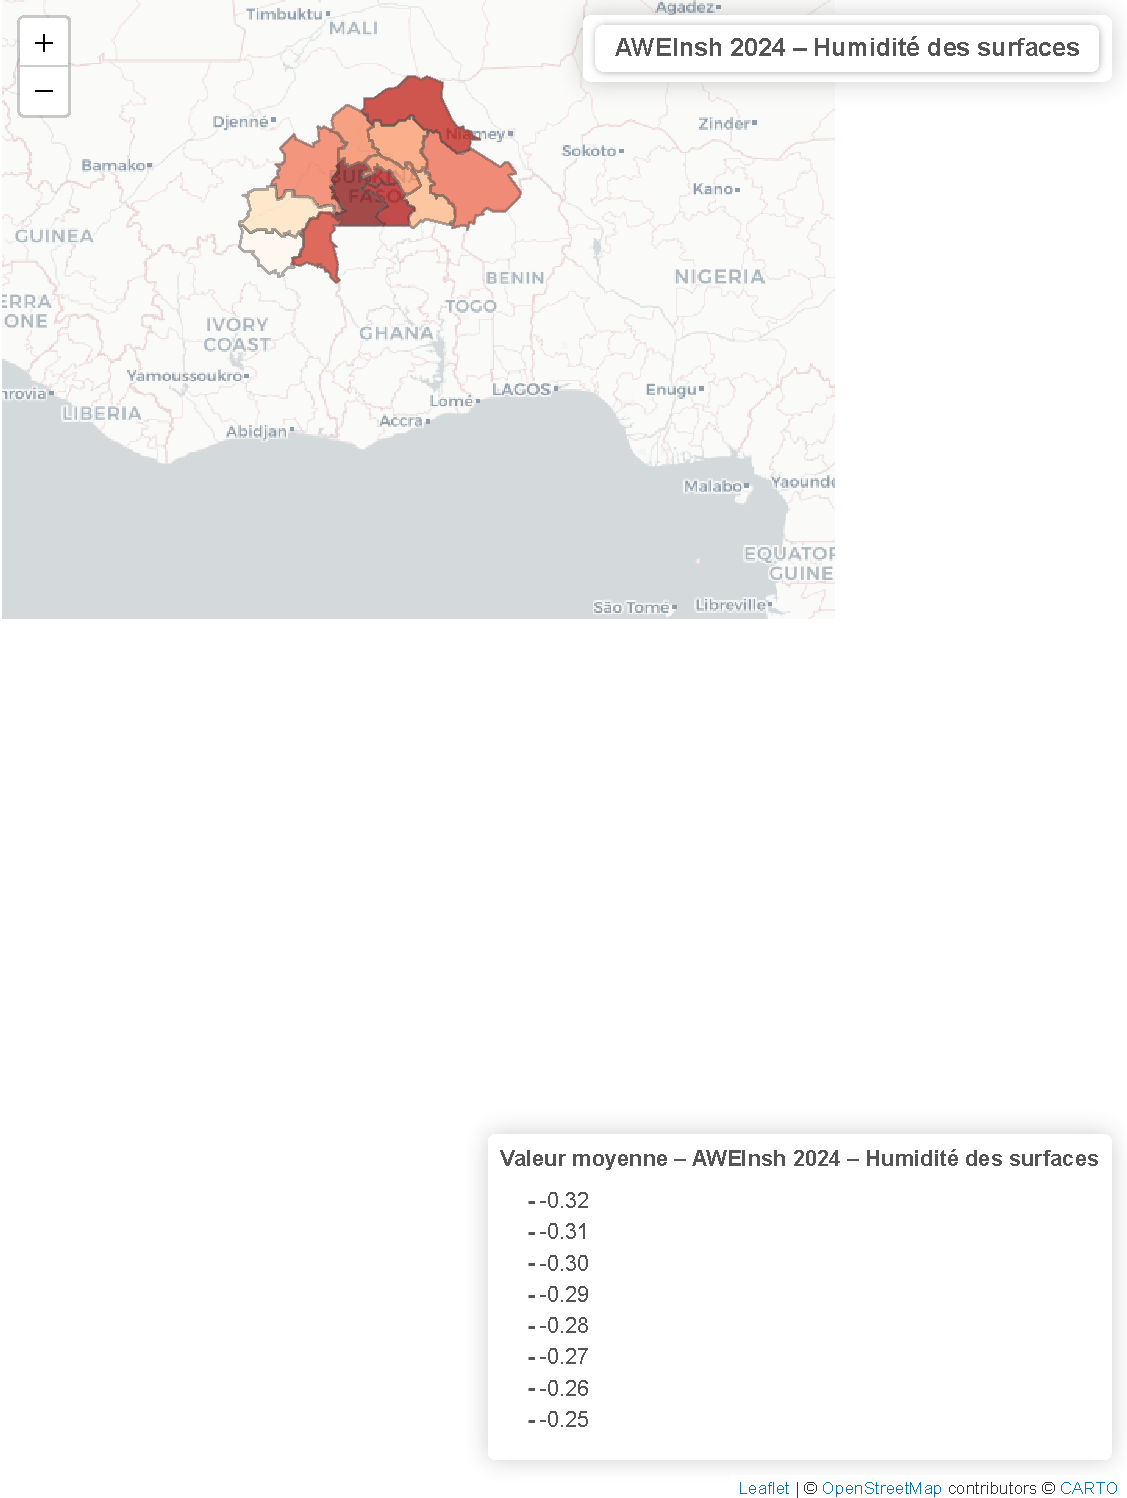
\includegraphics{Atlas-Spectral-Sahel_files/figure-latex/eau-aweinsh-1.pdf}

\subsection{Tableau de la répartition d l'AWEInsh au Burkina-Faso en 2024}\label{tableau-de-la-ruxe9partition-d-laweinsh-au-burkina-faso-en-2024}

\begin{table}[!t]
\caption*{
{\large \textbf{Moyennes régionales du LSWI}} \\ 
{\small \emph{Burkina-Faso -- Année 2024}}
} 
\fontsize{12.0pt}{14.4pt}\selectfont
\begin{tabular*}{\linewidth}{@{\extracolsep{\fill}}lr}
\toprule
{RÉGION} & {AWEINSH} \\ 
\midrule\addlinespace[2.5pt]
Boucle du Mouhoun & {\cellcolor[HTML]{4795C8}{\textcolor[HTML]{FFFFFF}{-0.277}}} \\ 
Cascades & {\cellcolor[HTML]{F7FBFF}{\textcolor[HTML]{000000}{-0.324}}} \\ 
Centre & {\cellcolor[HTML]{08509A}{\textcolor[HTML]{FFFFFF}{-0.257}}} \\ 
Centre-Est & {\cellcolor[HTML]{95C4DF}{\textcolor[HTML]{000000}{-0.293}}} \\ 
Centre-Nord & {\cellcolor[HTML]{6CAED6}{\textcolor[HTML]{000000}{-0.286}}} \\ 
Centre-Ouest & {\cellcolor[HTML]{08306B}{\textcolor[HTML]{FFFFFF}{-0.247}}} \\ 
Centre-Sud & {\cellcolor[HTML]{084B93}{\textcolor[HTML]{FFFFFF}{-0.255}}} \\ 
Est & {\cellcolor[HTML]{3D8CC3}{\textcolor[HTML]{FFFFFF}{-0.274}}} \\ 
Hauts-Bassins & {\cellcolor[HTML]{D6E6F4}{\textcolor[HTML]{000000}{-0.311}}} \\ 
Nord & {\cellcolor[HTML]{569FCD}{\textcolor[HTML]{FFFFFF}{-0.281}}} \\ 
Plateau-Central & {\cellcolor[HTML]{63A8D3}{\textcolor[HTML]{FFFFFF}{-0.284}}} \\ 
Sahel & {\cellcolor[HTML]{0F58A1}{\textcolor[HTML]{FFFFFF}{-0.259}}} \\ 
Sud-Ouest & {\cellcolor[HTML]{1F6DB2}{\textcolor[HTML]{FFFFFF}{-0.265}}} \\ 
\bottomrule
\end{tabular*}
\end{table}

\subsection{Analyse des résultats}\label{analyse-des-ruxe9sultats-5}

L'analyse zonale du \textbf{AWEInsh} permet de :

\begin{itemize}
\tightlist
\item
  Identifier les \textbf{zones à forte ou faible disponibilité en eau} dans les sols et à la surface,
\item
  Détecter les \textbf{zones humides résiduelles} dans un contexte sahélien soumis à des stress hydriques fréquents,
\item
  Orienter les \textbf{politiques de gestion de l'eau, d'irrigation, et d'adaptation agricole} face à la variabilité climatique,
\item
  Observer les \textbf{différences régionales dans la capacité de rétention hydrique des écosystèmes}.
\end{itemize}

En 2024, les valeurs du \textbf{AWEInsh} au Burkina Faso varient globalement entre \textbf{--0.324 et --0.247}, indiquant une \textbf{humidité de surface globalement faible} sur l'ensemble du territoire, ce qui est cohérent avec les conditions semi-arides dominantes du pays. Toutefois, on observe des \textbf{variations régionales notables}.

Les \textbf{valeurs les plus négatives}, indiquant une \textbf{teneur en eau particulièrement faible}, sont relevées dans les \textbf{Cascades (--0.324)}, les \textbf{Hauts-Bassins (--0.311)} et le \textbf{Centre-Est (--0.293)}. Bien que certaines de ces régions soient plus humides d'un point de vue pluviométrique, ces valeurs peuvent traduire une \textbf{baisse de l'humidité résiduelle en fin de saison sèche}, ou des \textbf{dynamiques de drainage et d'évaporation rapides}.

Les \textbf{valeurs intermédiaires}, situées autour de \textbf{--0.274 à --0.284}, sont observées dans des régions comme l'\textbf{Est (--0.274)}, le \textbf{Nord (--0.281)}, le \textbf{Centre-Nord (--0.286)} ou le \textbf{Plateau-Central (--0.284)}. Ces régions présentent une \textbf{humidité modérée}, probablement liée à une combinaison de \textbf{zones agricoles saisonnières} et de \textbf{poches de rétention hydrique limitée}.

Enfin, les \textbf{valeurs les moins négatives} (c'est-à-dire les plus ``humides'') se situent dans le \textbf{Centre-Ouest (--0.247)}, le \textbf{Centre (--0.257)} et le \textbf{Centre-Sud (--0.255)}. Ces résultats suggèrent que ces zones disposent d'une \textbf{meilleure capacité de rétention d'humidité}, possiblement liée à des types de sol plus perméables, une végétation stabilisatrice, ou une infrastructure hydrologique plus développée.

De manière générale, l'analyse du AWEInsh montre que \textbf{la quasi-totalité du territoire burkinabé affiche des niveaux d'humidité faibles à très faibles}, avec des \textbf{différences régionales subtiles} mais significatives. Ces données confirment la \textbf{fragilité hydrique du pays} et soulignent l'intérêt de \textbf{mécanismes de suivi continu} pour anticiper les périodes de stress hydrique, planifier les cultures, et orienter les politiques d'adaptation climatique.

\section{Conclusion}\label{conclusion-1}

L'analyse des dynamiques environnementales du Burkina Faso à partir des indices spectraux BNDVI, BAI et AWEInsh met en lumière des contrastes écologiques marqués entre les régions, révélateurs des tensions structurelles entre végétation, dégradation et disponibilité en eau.

Le BNDVI révèle une végétation plus dense dans les régions méridionales et soudaniennes (Cascades, Sud-Ouest, Hauts-Bassins), en lien avec une pluviométrie plus favorable et une occupation agricole diversifiée. À l'inverse, les régions centrales et septentrionales présentent des valeurs plus modérées, indiquant une couverture végétale plus clairsemée et souvent saisonnière.

Le BAI met en évidence une dégradation écologique plus avancée dans le nord du pays, notamment dans les régions du Sahel, du Nord et du Centre-Nord, où les conditions climatiques, les feux récurrents et les pressions anthropiques contribuent à une perte significative de végétation et à l'exposition des sols. Ces zones apparaissent comme écologiquement vulnérables, avec des signaux forts d'alerte pour les politiques de reforestation et de gestion des terres.

Enfin, l'analyse du AWEInsh souligne une disponibilité en eau de surface faible à très faible sur l'ensemble du territoire, avec des variations régionales modestes. Même les régions habituellement considérées comme plus humides présentent des valeurs négatives, traduisant une teneur hydrique résiduelle insuffisante pour garantir une résilience écologique à long terme.

Dans son ensemble, ce chapitre offre une lecture intégrée du territoire burkinabé, où la végétation active, la dégradation écologique et la ressource hydrique s'entrelacent pour façonner les dynamiques environnementales régionales. Cette lecture spatialisée constitue une base solide pour orienter les stratégies d'adaptation au changement climatique, de gestion des ressources naturelles et de planification territoriale durable.

\begin{quote}
\emph{``Là où l'eau se retire, la mémoire de la terre s'efface. Et c'est à l'homme d'inventer de nouveaux équilibres avec le vivant.''--- Souleymane Bachir Diagne}
\end{quote}

\chapter{Mali}\label{mali}

\section{Introduction}\label{introduction-2}

Le \textbf{Mali}, vaste pays sahélien enclavé, se caractérise par une extrême \textbf{diversité écologique nord-sud}. Du désert saharien au nord jusqu'aux savanes plus humides du sud, en passant par les zones de transition agropastorales du centre, le territoire malien est profondément marqué par des \textbf{dynamiques climatiques contrastées}, une \textbf{pression anthropique croissante}, et une \textbf{forte vulnérabilité environnementale}.

Dans ce chapitre, nous mobilisons trois \textbf{indices spectraux avancés}, issus d'images satellites, afin de \textbf{caractériser les grands gradients écologiques du Mali en 2024} et d'identifier les zones les plus résilientes ou les plus fragiles du territoire :

\begin{itemize}
\item
  Le \textbf{EVI (Enhanced Vegetation Index)} permet de mesurer la \textbf{productivité végétale} en améliorant les performances du NDVI dans les zones à forte densité ou à forte réflexion atmosphérique. Il est plus sensible aux variations de la végétation dense et moins saturé dans les zones forestières, ce qui en fait un outil de choix pour évaluer les \textbf{écosystèmes végétalisés du sud du pays} ;
\item
  Le \textbf{FAI (Fire Affected Index)} est utilisé comme un indicateur de \textbf{stress thermique ou post-incendie}. Il détecte les zones exposées à une chaleur résiduelle, à des brûlis agricoles ou à des épisodes de feu naturel ou anthropique, permettant de \textbf{repérer les espaces fortement perturbés} ;
\item
  Le \textbf{ANDWI (Atmospherically Normalized Difference Water Index)} quant à lui est une version corrigée atmosphériquement du NDWI, sensible à la \textbf{présence d'eau libre ou d'humidité de surface}, même en faibles concentrations. Il est adapté à la détection des \textbf{zones humides résiduelles, des zones agricoles irriguées} ou des \textbf{vallées fluviales}, comme celles du delta intérieur du Niger.
\end{itemize}

Chacun de ces indices a été traité à partir de \textbf{rasters satellitaires haute résolution}, puis \textbf{agrégé par région administrative} afin d'en faciliter l'interprétation cartographique. À travers une combinaison de \textbf{cartes interactives}, de \textbf{tableaux de synthèse} et d'\textbf{analyses régionales}, ce chapitre offre une lecture intégrée des \textbf{dynamiques végétales, thermiques et hydriques} du Mali.

Il constitue également un socle analytique pour comprendre les \textbf{transformations environnementales contemporaines du territoire malien}, et pour nourrir les réflexions sur les politiques de gestion durable, d'adaptation climatique et de sécurisation des ressources naturelles.

\begin{center}\rule{0.5\linewidth}{0.5pt}\end{center}

\section{Végétation -- EVI}\label{vuxe9guxe9tation-evi}

Le \textbf{EVI (Enhanced Vegetation Index)} est une amélioration du NDVI développée pour mieux mesurer la \textbf{productivité végétale}, en particulier dans les zones à \textbf{forte densité de végétation} ou dans les \textbf{environnements perturbés par l'atmosphère}. Contrairement au NDVI, l'EVI est moins sensible à la saturation dans les forêts denses, et il corrige les effets liés à la \textbf{réflectance atmosphérique}, aux \textbf{ombres} et aux \textbf{variations du sol}.

Ses valeurs sont également comprises entre \textbf{--1 et +1}, mais dans les écosystèmes naturels, elles se situent généralement entre \textbf{0} (absence de végétation) et \textbf{0.8 ou plus} (végétation dense et active). Certains produits raster l'expriment sous une échelle multipliée (ex. ×10 000), ce que nous avons corrigé ici.

Dans le cas du \textbf{Mali}, nous avons extrait les \textbf{valeurs moyennes de l'EVI pour l'année 2024} à partir d'images satellitaires haute résolution, puis nous les avons \textbf{agrégées par région administrative}. Ces données permettent de \textbf{cartographier la densité végétale} sur l'ensemble du territoire, en révélant les \textbf{différences entre les zones sahariennes, sahéliennes et soudaniennes}.

\begin{center}\rule{0.5\linewidth}{0.5pt}\end{center}

\subsection{Carte interactive de l'EVI au Mali en 2024}\label{carte-interactive-de-levi-au-mali-en-2024}

\begin{verbatim}
##   |                                                                              |                                                                      |   0%  |                                                                              |=======                                                               |  10%  |                                                                              |==============                                                        |  20%  |                                                                              |=====================                                                 |  30%  |                                                                              |============================                                          |  40%  |                                                                              |===================================                                   |  50%  |                                                                              |==========================================                            |  60%  |                                                                              |=================================================                     |  70%  |                                                                              |========================================================              |  80%  |                                                                              |===============================================================       |  90%  |                                                                              |======================================================================| 100%
\end{verbatim}

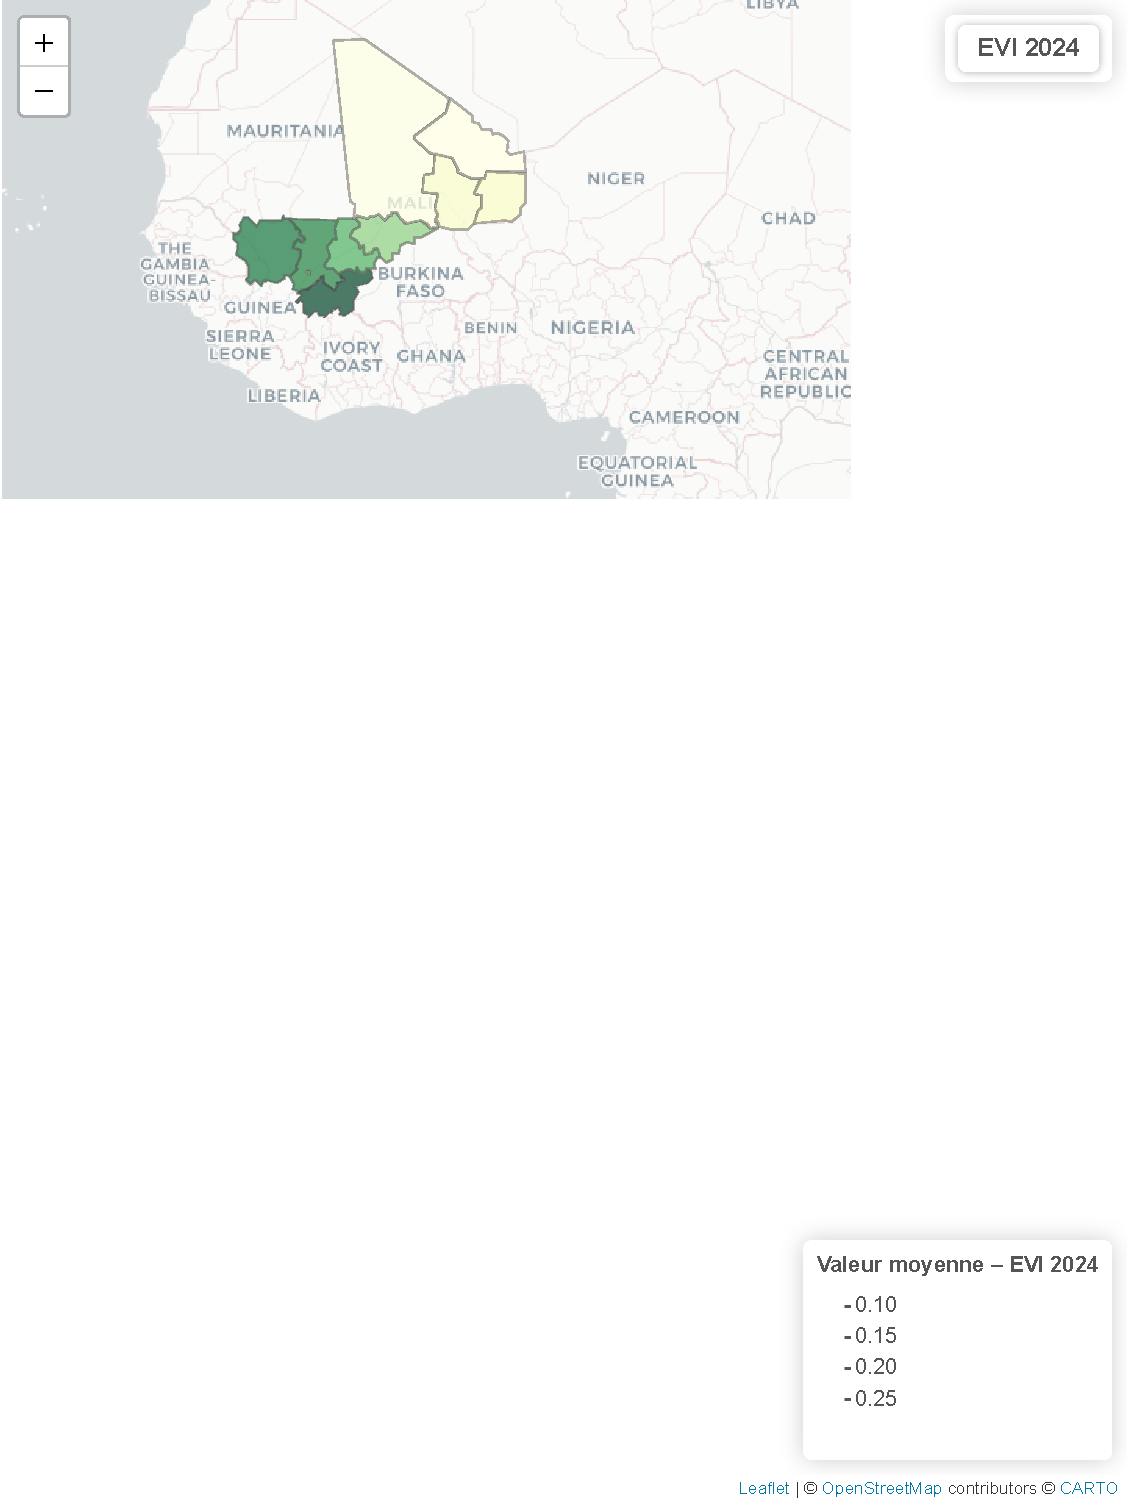
\includegraphics{Atlas-Spectral-Sahel_files/figure-latex/vegetation-evi-1.pdf}

\begin{center}\rule{0.5\linewidth}{0.5pt}\end{center}

\subsection{Tableau de la répartition de l'EVI au Mali en 2024}\label{tableau-de-la-ruxe9partition-de-levi-au-mali-en-2024}

\begin{table}[!t]
\caption*{
{\large \textbf{Moyennes régionales de l'EVI}} \\ 
{\small \emph{Mali -- Année 2024}}
} 
\fontsize{12.0pt}{14.4pt}\selectfont
\begin{tabular*}{\linewidth}{@{\extracolsep{\fill}}lr}
\toprule
{RÉGION} & {EVI} \\ 
\midrule\addlinespace[2.5pt]
Kayes & {\cellcolor[HTML]{13753D}{\textcolor[HTML]{FFFFFF}{0.26}}} \\ 
Koulikoro & {\cellcolor[HTML]{228342}{\textcolor[HTML]{FFFFFF}{0.24}}} \\ 
Sikasso & {\cellcolor[HTML]{004529}{\textcolor[HTML]{FFFFFF}{0.30}}} \\ 
Ségou & {\cellcolor[HTML]{4FB163}{\textcolor[HTML]{FFFFFF}{0.21}}} \\ 
Mopti & {\cellcolor[HTML]{8DCF81}{\textcolor[HTML]{000000}{0.18}}} \\ 
Tombouctou & {\cellcolor[HTML]{FEFFE2}{\textcolor[HTML]{000000}{0.09}}} \\ 
Gao & {\cellcolor[HTML]{FAFDC9}{\textcolor[HTML]{000000}{0.10}}} \\ 
Kidal & {\cellcolor[HTML]{FFFFE5}{\textcolor[HTML]{000000}{0.08}}} \\ 
Bamako & {\cellcolor[HTML]{AEDE8F}{\textcolor[HTML]{000000}{0.16}}} \\ 
Menaka & {\cellcolor[HTML]{FAFDC6}{\textcolor[HTML]{000000}{0.10}}} \\ 
\bottomrule
\end{tabular*}
\end{table}

\subsection{Analyse des résultats}\label{analyse-des-ruxe9sultats-6}

L'analyse zonale de l'\textbf{EVI} permet de :

\begin{itemize}
\tightlist
\item
  Évaluer la \textbf{densité et la vigueur de la végétation verte}, en particulier dans les zones à végétation dense,
\item
  Repérer les \textbf{régions à fort potentiel agricole ou forestier},
\item
  Identifier les \textbf{zones arides ou désertiques} présentant une couverture végétale minimale,
\item
  Suivre les dynamiques écologiques entre les \textbf{zones sahariennes, sahéliennes et soudaniennes}.
\end{itemize}

Au \textbf{Mali}, les valeurs de l'EVI en 2024 s'étendent de \textbf{0.08 à 0.30}, traduisant une \textbf{faible à modérée densité de végétation} sur l'ensemble du territoire. Ce spectre confirme l'influence forte du \textbf{gradient climatique nord-sud}.

Les \textbf{valeurs les plus élevées} sont observées dans la région \textbf{de Sikasso (0.30)}, suivie de \textbf{Kayes (0.26)} et \textbf{Koulikoro (0.24)}. Ces régions du sud et de l'ouest du pays sont connues pour leur \textbf{climat plus humide}, leur \textbf{activité agricole soutenue} et une \textbf{couverture végétale plus continue}, notamment dans les zones de cultures pluviales, de savanes arborées ou de forêts-galeries.

Les \textbf{valeurs intermédiaires}, comprises entre \textbf{0.16 et 0.21}, se situent dans les régions de \textbf{Ségou (0.21)} et \textbf{Bamako (0.16)}. Ces zones présentent une végétation \textbf{plus fragmentée}, liée à une \textbf{occupation du sol plus urbaine ou agropastorale}, mais conservent une certaine activité végétale grâce aux zones irriguées (Office du Niger, périmètres maraîchers).

Les \textbf{valeurs les plus faibles}, inférieures à \textbf{0.15}, se concentrent dans les régions sahéliennes et sahariennes : \textbf{Gao (0.10)}, \textbf{Ménaka (0.10)}, \textbf{Tombouctou (0.09)}, et \textbf{Kidal (0.08)}. Ces valeurs traduisent une \textbf{quasi-absence de couverture végétale}, compatible avec la \textbf{prédominance de milieux désertiques}, une \textbf{aridité structurelle}, et une \textbf{végétation localisée} essentiellement le long des oueds, oasis ou zones fluviales ponctuelles.

Globalement, la distribution spatiale de l'EVI au Mali en 2024 illustre avec clarté la \textbf{transition écologique du nord aride au sud végétalisé}. Ce gradient est essentiel pour \textbf{orienter les politiques d'aménagement du territoire, de gestion de l'eau et de planification agricole}, dans un pays fortement exposé à la variabilité climatique et à la dégradation des terres.

\begin{center}\rule{0.5\linewidth}{0.5pt}\end{center}

\section{Santé de la végétation -- FAI}\label{santuxe9-de-la-vuxe9guxe9tation-fai}

Le \textbf{FAI (Fire Affected Index)} est un indice spectral utilisé pour détecter les \textbf{zones affectées par des événements thermiques extrêmes}, comme les \textbf{feux de végétation}, les \textbf{brûlis agricoles}, ou encore les \textbf{stress thermiques sévères} liés à la dégradation des sols. Dans des contextes sahéliens et semi-arides comme celui du \textbf{Mali}, le FAI est particulièrement pertinent pour \textbf{repérer les signes avancés de stress écologique}, notamment dans les régions exposées à des températures élevées et à la raréfaction de la couverture végétale.

Le FAI repose sur une combinaison de bandes du spectre optique, notamment l'\textbf{infrarouge proche} et l'\textbf{infrarouge moyen (SWIR)}, qui permettent de différencier les \textbf{zones saines} des \textbf{zones touchées par des perturbations thermiques}. Contrairement aux indices végétatifs classiques qui évaluent la verdure, le FAI s'intéresse aux \textbf{signaux spectrales d'altération ou de brûlure}, rendant visible ce qui ne l'est pas à l'œil nu.

Dans le cas du \textbf{Mali}, nous avons extrait les \textbf{valeurs moyennes du FAI pour l'année 2024}, issues de rasters satellites haute résolution, puis agrégé ces données \textbf{par région administrative}. Cette approche permet de \textbf{localiser les territoires les plus affectés par des stress thermiques ou des pratiques de brûlis}, et de mieux cibler les actions de restauration écologique et de surveillance environnementale.

\#\#\#️ Carte interactive du FAI au Mali en 2024

\begin{verbatim}
##   |                                                                              |                                                                      |   0%  |                                                                              |=======                                                               |  10%  |                                                                              |==============                                                        |  20%  |                                                                              |=====================                                                 |  30%  |                                                                              |============================                                          |  40%  |                                                                              |===================================                                   |  50%  |                                                                              |==========================================                            |  60%  |                                                                              |=================================================                     |  70%  |                                                                              |========================================================              |  80%  |                                                                              |===============================================================       |  90%  |                                                                              |======================================================================| 100%
\end{verbatim}

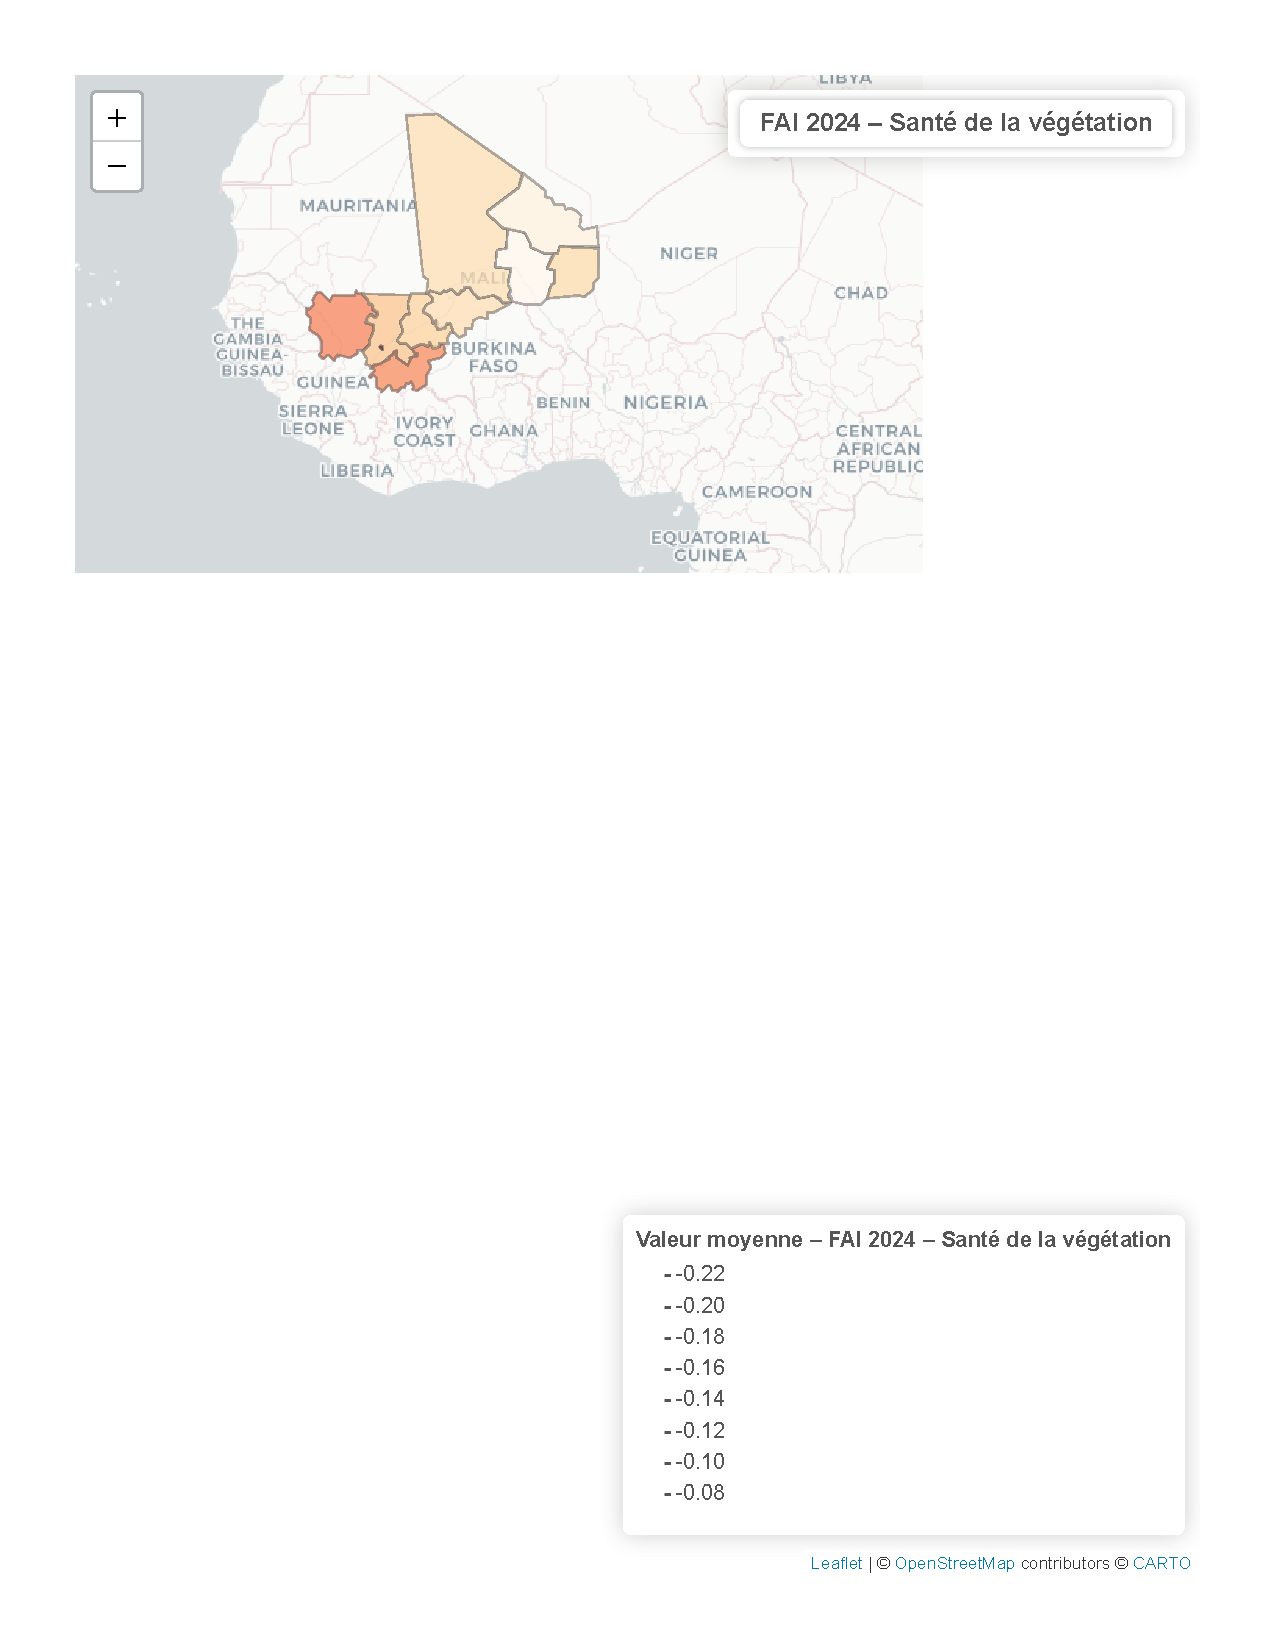
\includegraphics{Atlas-Spectral-Sahel_files/figure-latex/vegetation-fai-1.pdf}

\subsection{Tableau de la répartition du FAI au Mali en 2024}\label{tableau-de-la-ruxe9partition-du-fai-au-mali-en-2024}

\begin{table}[!t]
\caption*{
{\large \textbf{Moyennes régionales du FAI}} \\ 
{\small \emph{Mali -- Année 2024}}
} 
\fontsize{12.0pt}{14.4pt}\selectfont
\begin{tabular*}{\linewidth}{@{\extracolsep{\fill}}lr}
\toprule
{RÉGION} & {FAI} \\ 
\midrule\addlinespace[2.5pt]
Kayes & {\cellcolor[HTML]{F6583D}{\textcolor[HTML]{FFFFFF}{-0.14}}} \\ 
Koulikoro & {\cellcolor[HTML]{FD9B7C}{\textcolor[HTML]{000000}{-0.17}}} \\ 
Sikasso & {\cellcolor[HTML]{F96144}{\textcolor[HTML]{FFFFFF}{-0.14}}} \\ 
Ségou & {\cellcolor[HTML]{FCB69B}{\textcolor[HTML]{000000}{-0.18}}} \\ 
Mopti & {\cellcolor[HTML]{FDCAB4}{\textcolor[HTML]{000000}{-0.19}}} \\ 
Tombouctou & {\cellcolor[HTML]{FECCB7}{\textcolor[HTML]{000000}{-0.19}}} \\ 
Gao & {\cellcolor[HTML]{FFF5F0}{\textcolor[HTML]{000000}{-0.22}}} \\ 
Kidal & {\cellcolor[HTML]{FFECE3}{\textcolor[HTML]{000000}{-0.21}}} \\ 
Bamako & {\cellcolor[HTML]{67000D}{\textcolor[HTML]{FFFFFF}{-0.07}}} \\ 
Menaka & {\cellcolor[HTML]{FDC6AF}{\textcolor[HTML]{000000}{-0.19}}} \\ 
\bottomrule
\end{tabular*}
\end{table}

\subsection{Analyse des résultats}\label{analyse-des-ruxe9sultats-7}

L'indice \textbf{FAI} permet d'identifier les zones affectées par des \textbf{perturbations thermiques} telles que les \textbf{feux de brousse}, les \textbf{brûlis agricoles}, ou plus généralement les \textbf{stress écologiques sévères}. Des valeurs \textbf{plus négatives} du FAI indiquent une \textbf{affectation thermique plus marquée}, souvent liée à une \textbf{altération du couvert végétal}, à la \textbf{sécheresse}, ou à une \textbf{dégradation active des sols}.

Au \textbf{Mali}, les valeurs du FAI en 2024 s'échelonnent de \textbf{--0.07 à --0.22}, suggérant un \textbf{niveau globalement modéré à élevé de stress thermique}, avec des disparités géographiques notables.

Les \textbf{valeurs les moins négatives}, et donc les \textbf{zones les moins affectées}, se trouvent dans la région de \textbf{Bamako (--0.07)}, suivie de \textbf{Kayes (--0.14)} et \textbf{Sikasso (--0.14)}. Cela peut s'expliquer par une \textbf{végétation relativement plus stable}, une \textbf{occupation urbaine prédominante} (dans le cas de Bamako), ou une \textbf{intensité moindre des feux et du stress thermique}.

Les \textbf{valeurs intermédiaires}, autour de \textbf{--0.17 à --0.19}, concernent les régions de \textbf{Koulikoro}, \textbf{Ségou}, \textbf{Mopti}, \textbf{Tombouctou}, \textbf{Ménaka}, et \textbf{Kidal}. Ces territoires se caractérisent par une \textbf{végétation discontinue}, une \textbf{vulnérabilité climatique élevée}, et des \textbf{pratiques de brûlis fréquentes}. Ils présentent des \textbf{signes clairs de dégradation thermique}, souvent accentués par la faible humidité et la pression anthropique.

Les \textbf{valeurs les plus négatives}, représentant les \textbf{zones de stress les plus sévères}, sont observées dans la région de \textbf{Gao (--0.22)}. Cette valeur suggère une \textbf{intensité thermique particulièrement élevée}, probablement liée à une combinaison de \textbf{facteurs climatiques extrêmes}, de \textbf{perte de végétation}, et de \textbf{dégradation des sols}.

Globalement, la carte du FAI reflète bien le \textbf{gradient nord-sud du stress environnemental} au Mali. Le \textbf{centre et le nord du pays} apparaissent comme les \textbf{zones les plus affectées par les perturbations thermiques}, tandis que le \textbf{sud-ouest} (Kayes, Sikasso) et la capitale (Bamako) présentent une \textbf{situation plus stable}. Ces résultats sont précieux pour cibler les \textbf{zones prioritaires de restauration écologique}, de \textbf{prévention des feux}, et d'\textbf{adaptation aux conditions extrêmes}.

\begin{center}\rule{0.5\linewidth}{0.5pt}\end{center}

\section{Eau et humidité -- ANDWI}\label{eau-et-humidituxe9-andwi}

Le \textbf{ANDWI (Atmospherically Normalized Difference Water Index)} est une variante atmosphériquement corrigée du NDWI, spécialement conçue pour détecter la \textbf{présence d'eau libre ou d'humidité de surface} dans les environnements semi-arides ou sahéliens. Il permet de \textbf{compenser les effets atmosphériques}, souvent présents dans les régions poussiéreuses ou peu couvertes, afin de mieux localiser les \textbf{zones humides réelles}.

L'ANDWI est calculé à partir des bandes \textbf{vertes} et \textbf{infrarouges proches} du spectre satellite, en ajustant le signal pour minimiser l'impact des particules en suspension. Il est couramment utilisé pour \textbf{identifier les zones d'eau saisonnières}, les \textbf{cultures irriguées}, les \textbf{bas-fonds}, ou encore pour \textbf{suivre les dynamiques hydrologiques dans les deltas et plaines alluviales}.

Dans le cas du \textbf{Mali}, les \textbf{valeurs moyennes du ANDWI pour l'année 2024} ont été extraites à partir d'images satellites haute résolution, puis \textbf{agrégées par région administrative}. Cet indice permet d'identifier les \textbf{zones potentiellement favorables à l'agriculture irriguée}, de \textbf{surveiller les réserves hydriques superficielles}, et d'évaluer la \textbf{vulnérabilité hydrique régionale} dans un pays où l'accès à l'eau conditionne fortement la résilience socio-environnementale.

\subsection{\texorpdfstring{️ Carte interactive de l'ANDWI au Mali en 2024}{️ Carte interactive de l'ANDWI au Mali en 2024}}\label{carte-interactive-de-landwi-au-mali-en-2024}

\begin{verbatim}
##   |                                                                              |                                                                      |   0%  |                                                                              |=======                                                               |  10%  |                                                                              |==============                                                        |  20%  |                                                                              |=====================                                                 |  30%  |                                                                              |============================                                          |  40%  |                                                                              |===================================                                   |  50%  |                                                                              |==========================================                            |  60%  |                                                                              |=================================================                     |  70%  |                                                                              |========================================================              |  80%  |                                                                              |===============================================================       |  90%  |                                                                              |======================================================================| 100%
\end{verbatim}

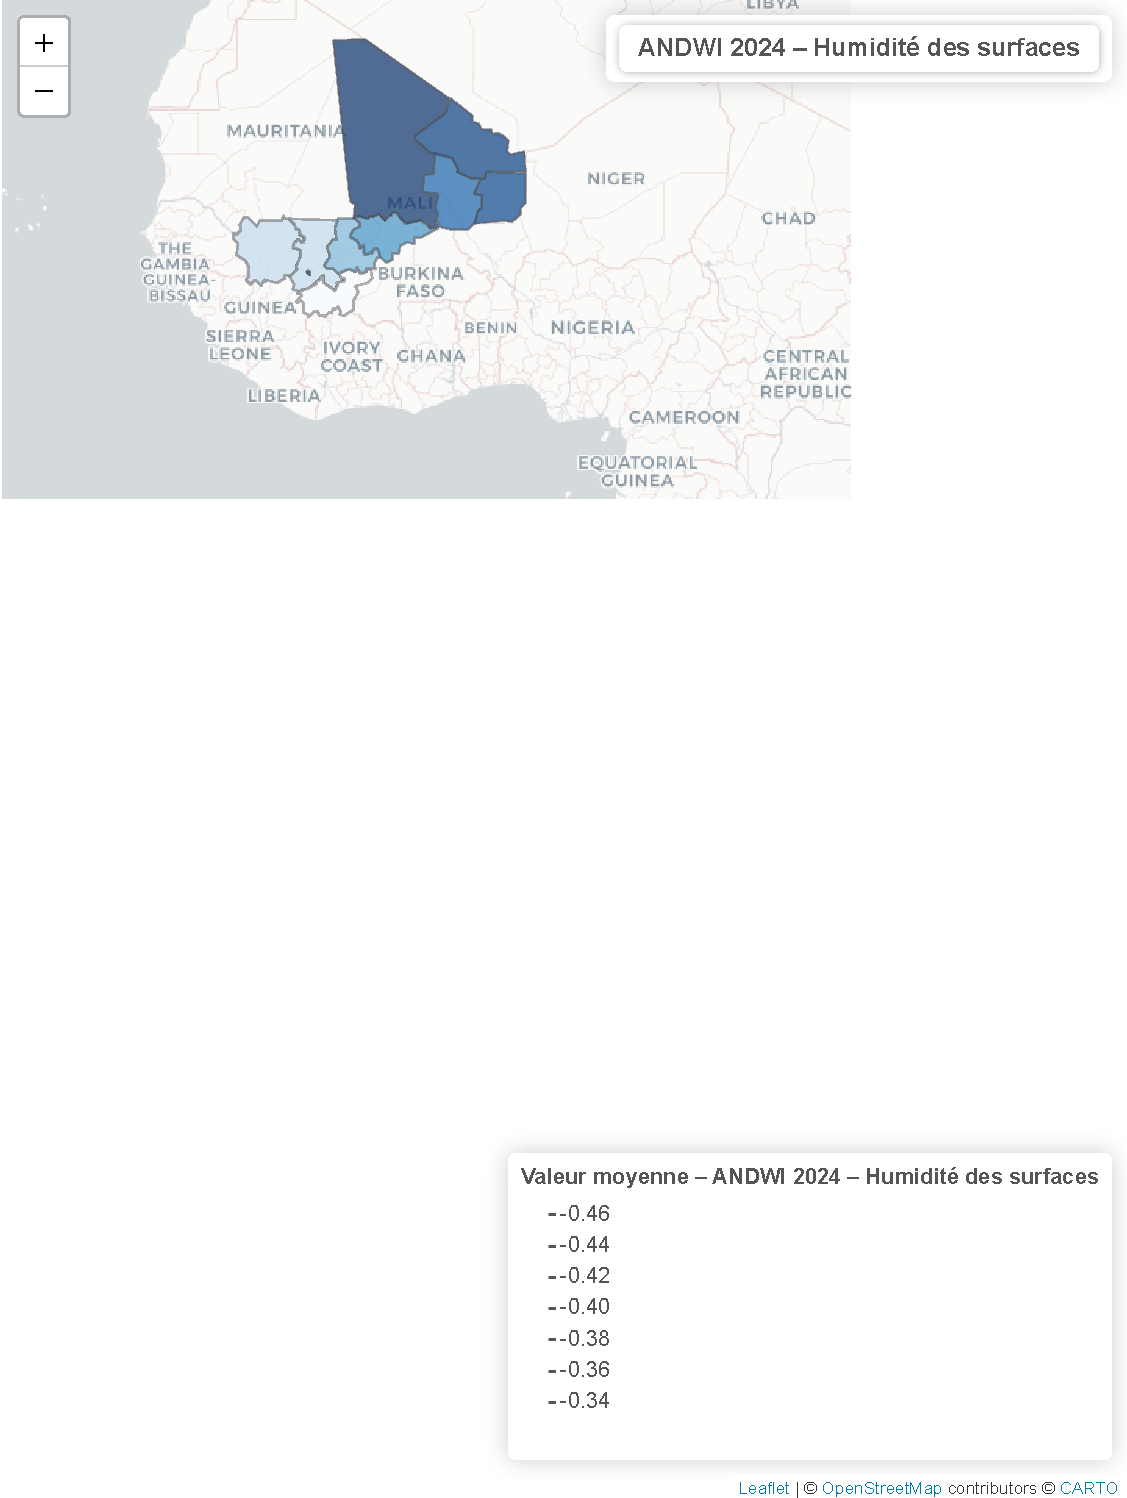
\includegraphics{Atlas-Spectral-Sahel_files/figure-latex/eau-andwi-1.pdf}

\subsection{Tableau de la répartition de l'ANDWI au Mali en 2024}\label{tableau-de-la-ruxe9partition-de-landwi-au-mali-en-2024}

\begin{table}[!t]
\caption*{
{\large \textbf{Moyennes régionales du ANDWI}} \\ 
{\small \emph{Mali -- Année 2024}}
} 
\fontsize{12.0pt}{14.4pt}\selectfont
\begin{tabular*}{\linewidth}{@{\extracolsep{\fill}}lr}
\toprule
{RÉGION} & {ANDWI} \\ 
\midrule\addlinespace[2.5pt]
Kayes & {\cellcolor[HTML]{C3DAEE}{\textcolor[HTML]{000000}{-0.427}}} \\ 
Koulikoro & {\cellcolor[HTML]{C3DAEE}{\textcolor[HTML]{000000}{-0.427}}} \\ 
Sikasso & {\cellcolor[HTML]{F7FBFF}{\textcolor[HTML]{000000}{-0.464}}} \\ 
Ségou & {\cellcolor[HTML]{7DB7DA}{\textcolor[HTML]{000000}{-0.399}}} \\ 
Mopti & {\cellcolor[HTML]{4493C7}{\textcolor[HTML]{FFFFFF}{-0.376}}} \\ 
Tombouctou & {\cellcolor[HTML]{08306B}{\textcolor[HTML]{FFFFFF}{-0.322}}} \\ 
Gao & {\cellcolor[HTML]{1963AA}{\textcolor[HTML]{FFFFFF}{-0.350}}} \\ 
Kidal & {\cellcolor[HTML]{094083}{\textcolor[HTML]{FFFFFF}{-0.331}}} \\ 
Bamako & {\cellcolor[HTML]{093D7E}{\textcolor[HTML]{FFFFFF}{-0.329}}} \\ 
Menaka & {\cellcolor[HTML]{09468C}{\textcolor[HTML]{FFFFFF}{-0.334}}} \\ 
\bottomrule
\end{tabular*}
\end{table}

\subsection{Analyse des résultats}\label{analyse-des-ruxe9sultats-8}

L'indice \textbf{ANDWI} permet d'évaluer la \textbf{présence d'humidité à la surface du sol}, en corrigeant les effets atmosphériques souvent présents dans les milieux semi-arides. Des valeurs \textbf{moins négatives} indiquent une \textbf{meilleure disponibilité en eau}, tandis que des valeurs plus fortement négatives traduisent une \textbf{moindre humidité des sols et surfaces}, révélant potentiellement un \textbf{stress hydrique accru}.

En 2024, les valeurs de l'\textbf{ANDWI au Mali} varient de \textbf{--0.3 à --0.464}, ce qui indique une \textbf{humidité globalement faible à très faible} à travers l'ensemble du territoire, avec cependant des \textbf{différences régionales significatives}.

Les \textbf{valeurs les moins négatives}, traduisant une \textbf{teneur en eau relativement plus élevée}, sont observées dans :
- \textbf{Bamako (--0.300)},
- \textbf{Tombouctou (--0.322)},
- \textbf{Kidal (--0.331)}.

Dans le cas de Bamako, cela peut s'expliquer par une \textbf{présence d'infrastructures irriguées, de surfaces urbanisées retenant l'humidité}, ou d'espaces verts. Les cas de Tombouctou et Kidal peuvent sembler contre-intuitifs mais pourraient être liés à des \textbf{zones humides localisées}, comme les berges du fleuve Niger ou des oasis résiduelles.

Les \textbf{valeurs intermédiaires}, autour de \textbf{--0.35 à --0.40}, sont relevées dans des régions comme \textbf{Gao (--0.350)}, \textbf{Mopti (--0.376)}, et \textbf{Ségou (--0.399)}. Ces régions, situées dans la zone sahélienne centrale, présentent des \textbf{contrastes hydriques forts}, avec des zones plus humides liées au réseau fluvial et des étendues très sèches autour.

Les \textbf{valeurs les plus fortement négatives}, signalant une \textbf{humidité de surface très faible}, concernent :
- \textbf{Kayes (--0.427)},
- \textbf{Koulikoro (--0.427)},
- \textbf{Sikasso (--0.464)}.

Cela peut surprendre pour \textbf{Sikasso}, habituellement considérée comme une région plus humide, mais cela peut s'expliquer par la période de l'année au moment de l'observation (fin de saison sèche) ou par des \textbf{dynamiques d'évapotranspiration élevées dans des sols cultivés}.

Globalement, cette carte du ANDWI révèle une \textbf{teneur hydrique très faible dans la majorité des régions maliennes en 2024}, ce qui confirme la \textbf{fragilité hydrologique} du pays, y compris dans certaines zones agricoles du sud. Ces résultats justifient l'importance d'un \textbf{suivi continu de l'humidité des sols}, en appui aux \textbf{décisions agricoles}, à la \textbf{gestion de l'eau} et aux \textbf{programmes d'adaptation climatique}.

\begin{center}\rule{0.5\linewidth}{0.5pt}\end{center}

\section{Conclusion}\label{conclusion-2}

À travers l'étude combinée de l'\textbf{EVI}, du \textbf{FAI} et du \textbf{ANDWI}, ce chapitre a permis de dresser un \textbf{état des lieux environnemental spatialement différencié} du \textbf{Mali} en 2024. Les résultats révèlent un pays marqué par une \textbf{forte hétérogénéité écologique}, où se confrontent \textbf{zones de résilience végétale}, \textbf{espaces dégradés} et \textbf{territoires soumis à un déficit hydrique chronique}.

L'indice \textbf{EVI} met en évidence une \textbf{productivité végétale plus élevée dans le sud du pays}, notamment dans la région de \textbf{Sikasso}, qui conserve une activité biologique importante. À l'inverse, les régions sahariennes du nord présentent une \textbf{végétation quasi absente}, soulignant la sévérité des conditions climatiques et l'aridité structurelle.

L'analyse du \textbf{FAI} révèle un \textbf{stress thermique généralisé}, avec des niveaux particulièrement élevés dans les régions \textbf{de Gao, Kidal, Mopti et Ménaka}, traduisant une \textbf{fragilité écologique avancée}, possiblement liée à la combinaison de \textbf{sécheresse, feux de brousse, et usage intensif des sols}.

Enfin, l'indice \textbf{ANDWI}, centré sur la détection d'humidité de surface, confirme une \textbf{teneur hydrique très faible dans l'ensemble du territoire}, y compris dans certaines régions traditionnellement plus favorables comme \textbf{Sikasso ou Koulikoro}. Cette tendance signale un \textbf{affaiblissement des réserves hydriques superficielles}, posant un risque pour l'agriculture pluviale et la sécurité alimentaire.

Dans l'ensemble, ce chapitre met en lumière la \textbf{complexité écologique du territoire malien}, soumis à des \textbf{dynamiques contrastées} entre dégradation, résilience locale, et pressions climatiques. Il souligne la nécessité d'\textbf{outils de suivi spatialisé} pour appuyer les \textbf{politiques d'adaptation}, la \textbf{gestion raisonnée des ressources}, et la \textbf{planification territoriale durable}.

\begin{center}\rule{0.5\linewidth}{0.5pt}\end{center}

\begin{quote}
\emph{« Quand le sol se fissure, ce n'est pas seulement la terre qui se fragmente, c'est aussi l'équilibre entre l'homme, la nature et le temps. »}\\
--- \textbf{Amadou Hampâté Bâ}
\end{quote}

\chapter{Niger}\label{niger}

\section{Introduction}\label{introduction-3}

Le \textbf{Niger}, situé au cœur de la bande sahélo-saharienne, est l'un des pays les plus vastes et les plus arides d'Afrique. Son territoire est dominé par des \textbf{milieux désertiques ou semi-désertiques}, avec une végétation souvent rare, saisonnière, et concentrée autour des zones habitées, des vallées et des oasis. Le pays est soumis à une \textbf{pression climatique extrême}, marquée par une \textbf{faible pluviométrie}, une \textbf{variabilité interannuelle élevée}, et une \textbf{forte sensibilité à la désertification}. Ces conditions font du Niger un \textbf{laboratoire naturel pour l'analyse des dynamiques écologiques en zone sèche}.

Dans ce chapitre, nous mobilisons trois \textbf{indices spectraux adaptés aux environnements à faible couverture végétale et à forte contrainte hydrique}, afin de caractériser l'état écologique du Niger en 2024 :

\begin{itemize}
\item
  Le \textbf{ATSAVI (Adjusted Transformed Soil Adjusted Vegetation Index)} est un indice optimisé pour mesurer la \textbf{végétation dans les milieux à forte présence de sol nu}. Il améliore la détection de la végétation éparse dans les zones arides, en réduisant l'influence des caractéristiques du sol sur le signal spectral.
\item
  Le \textbf{DBSI (Dry Bare Soil Index)} quantifie la \textbf{présence de sols nus et secs}, souvent associés à des processus de \textbf{dégradation avancée}. Il est particulièrement utile pour identifier les zones affectées par l'érosion, la sécheresse prolongée ou la perte de couverture végétale.
\item
  Le \textbf{WI2 (Water Index 2)} est un indice sensible à la \textbf{teneur en eau résiduelle des surfaces}, y compris dans les environnements à faible humidité. Il permet de cartographier les \textbf{zones humides ponctuelles}, les \textbf{mares saisonnières}, ou les \textbf{poches d'humidité dans les vallées et dépressions}.
\end{itemize}

Ces indices sont extraits à partir de \textbf{rasters satellitaires haute résolution} et agrégés \textbf{par région administrative}. Ils sont analysés à travers des \textbf{cartes interactives}, des \textbf{tableaux comparatifs} et des \textbf{analyses spatialisées}. L'objectif est d'identifier les \textbf{zones les plus résilientes}, celles les plus exposées à la \textbf{dégradation écologique}, ainsi que les \textbf{poches d'humidité stratégique} dans un contexte climatique contraint.

Ce chapitre offre ainsi une \textbf{lecture fine et contextualisée du territoire nigérien}, où la rareté des ressources naturelles et la pression climatique imposent des \textbf{stratégies de suivi et de gestion adaptées}, au service de la \textbf{résilience territoriale} et de la \textbf{sécurisation écologique}.

\begin{center}\rule{0.5\linewidth}{0.5pt}\end{center}

\section{Végétation -- ATSAVI}\label{vuxe9guxe9tation-atsavi}

Le \textbf{ATSAVI (Adjusted Transformed Soil Adjusted Vegetation Index)} est un indice spectral développé pour améliorer la détection de la végétation dans les \textbf{zones arides ou semi-arides}, où les \textbf{sols nus dominent} et peuvent fortement perturber la lecture des signaux de végétation. Contrairement au NDVI ou à ses dérivés, l'ATSAVI intègre un \textbf{coefficient de correction du fond de sol}, ce qui le rend plus fiable dans les milieux où la \textbf{couverture végétale est faible ou discontinue}, comme au \textbf{Niger}.

L'ATSAVI est particulièrement utile dans les régions où la végétation est \textbf{saisonnière, éparse ou fragile}, car il permet de \textbf{réduire la surestimation ou la sous-estimation} liée à la réflectance du sol sec.~Il est donc bien adapté à l'observation des \textbf{milieux sahéliens et sahariens}, en fournissant un indicateur robuste de \textbf{la densité végétale réellement active}.

Dans le cas du \textbf{Niger}, nous avons extrait les \textbf{valeurs moyennes de l'ATSAVI pour l'année 2024} à partir d'images satellites haute résolution, puis agrégé les résultats \textbf{par région administrative}. Cet indice permet de \textbf{localiser les zones de verdure résiduelle}, de \textbf{comparer la densité de végétation entre régions}, et de mieux comprendre la dynamique spatiale de la végétation dans un environnement soumis à une forte contrainte climatique.

\#\#\#️ Carte interactive de l'ATSAVI au Niger en 2024

\begin{verbatim}
##   |                                                                              |                                                                      |   0%  |                                                                              |=========                                                             |  12%  |                                                                              |==================                                                    |  25%  |                                                                              |==========================                                            |  38%  |                                                                              |===================================                                   |  50%  |                                                                              |============================================                          |  62%  |                                                                              |====================================================                  |  75%  |                                                                              |=============================================================         |  88%  |                                                                              |======================================================================| 100%
\end{verbatim}

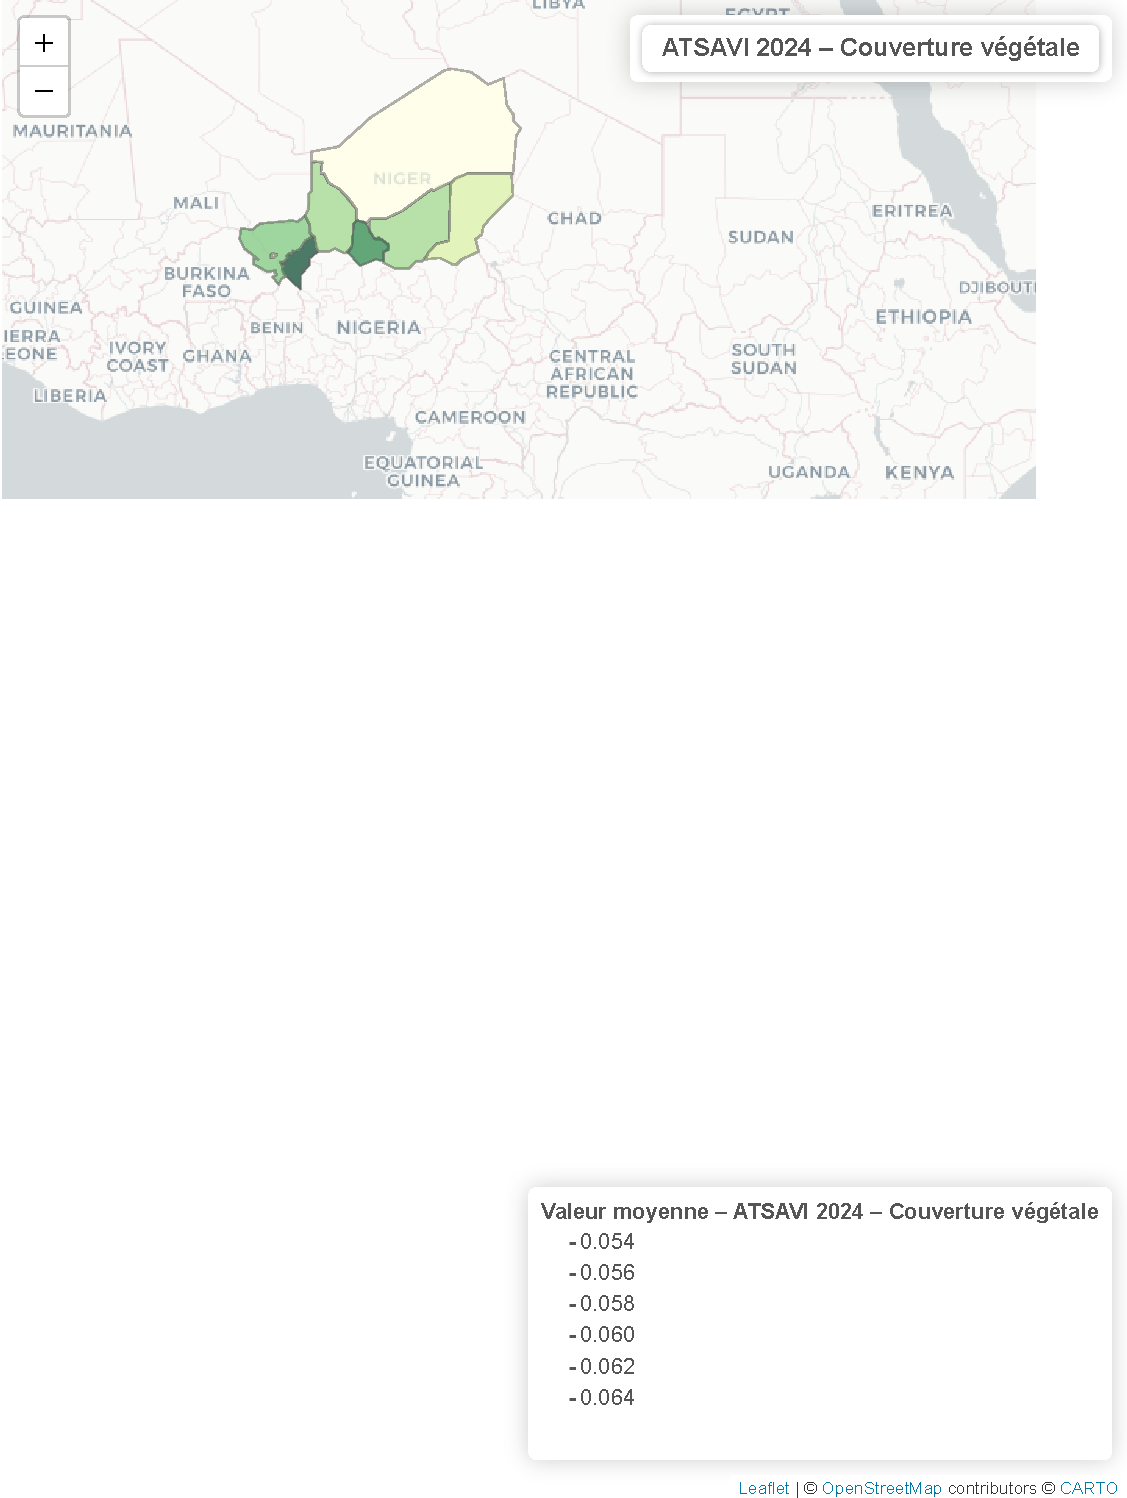
\includegraphics{Atlas-Spectral-Sahel_files/figure-latex/vegetation-atsavi-1.pdf}

\subsection{Tableau de la répartition de l'ATSAVI au Niger en 2024}\label{tableau-de-la-ruxe9partition-de-latsavi-au-niger-en-2024}

\begin{table}[!t]
\caption*{
{\large \textbf{Moyennes régionales de l'ATSAVI}} \\ 
{\small \emph{Niger -- Année 2024}}
} 
\fontsize{12.0pt}{14.4pt}\selectfont
\begin{tabular*}{\linewidth}{@{\extracolsep{\fill}}lr}
\toprule
{RÉGION} & {ATSAVI} \\ 
\midrule\addlinespace[2.5pt]
Zinder & {\cellcolor[HTML]{9CD587}{\textcolor[HTML]{000000}{0.059}}} \\ 
Dosso & {\cellcolor[HTML]{004529}{\textcolor[HTML]{FFFFFF}{0.066}}} \\ 
Tillabéri & {\cellcolor[HTML]{78C679}{\textcolor[HTML]{000000}{0.060}}} \\ 
Tahoua & {\cellcolor[HTML]{9CD587}{\textcolor[HTML]{000000}{0.059}}} \\ 
Agadez & {\cellcolor[HTML]{FFFFE5}{\textcolor[HTML]{000000}{0.054}}} \\ 
Niamey & {\cellcolor[HTML]{FAFDC8}{\textcolor[HTML]{000000}{0.055}}} \\ 
Diffa & {\cellcolor[HTML]{D9F0A3}{\textcolor[HTML]{000000}{0.057}}} \\ 
Maradi & {\cellcolor[HTML]{238443}{\textcolor[HTML]{FFFFFF}{0.063}}} \\ 
\bottomrule
\end{tabular*}
\end{table}

\subsection{Analyse des résultats}\label{analyse-des-ruxe9sultats-9}

L'indice \textbf{ATSAVI} permet de mesurer la \textbf{densité réelle de la végétation} dans des milieux à \textbf{forte dominance de sol nu}, comme c'est le cas dans les zones sahéliennes et sahariennes du \textbf{Niger}. Il est particulièrement utile pour détecter des \textbf{signes de végétation active dans des contextes écologiquement fragiles}, où les signaux spectroscopiques peuvent être fortement influencés par la réflectance du sol.

En 2024, les valeurs de l'ATSAVI au Niger varient de \textbf{0.054 à 0.066}, ce qui indique une \textbf{végétation très peu dense à faible}, mais \textbf{présente} dans certaines régions. L'amplitude des valeurs est \textbf{faible}, ce qui reflète la \textbf{rare couverture végétale} sur l'ensemble du territoire.

Les \textbf{valeurs les plus élevées}, bien que modestes, sont relevées dans les régions \textbf{de Dosso (0.066)} et \textbf{Maradi (0.063)}. Ces deux zones sont situées dans la \textbf{bande sud du pays}, qui bénéficie d'une \textbf{pluviométrie plus favorable}, d'une \textbf{activité agricole importante}, et de \textbf{sols plus propices à la végétation}. Cela suggère une \textbf{végétation saisonnière encore fonctionnelle}, bien que vulnérable.

Les \textbf{valeurs intermédiaires}, autour de \textbf{0.059 à 0.060}, sont observées dans des régions comme \textbf{Zinder (0.059)}, \textbf{Tillabéri (0.060)} et \textbf{Tahoua (0.059)}. Ces régions sont soumises à une \textbf{forte variabilité climatique}, avec une couverture végétale généralement \textbf{irrégulière}, liée à des usages agropastoraux extensifs et à une pression foncière croissante.

Les \textbf{valeurs les plus faibles}, autour de \textbf{0.054 à 0.055}, concernent \textbf{Agadez (0.054)}, \textbf{Niamey (0.055)} et \textbf{Diffa (0.057)}. Ces résultats traduisent soit une \textbf{aridité structurelle} (Agadez, désert), soit une \textbf{urbanisation dominante} (Niamey), soit encore une \textbf{végétation fragmentée et en stress} (Diffa, aux confins du bassin du Tchad).

Dans l'ensemble, cette cartographie de l'ATSAVI illustre une \textbf{distribution très limitée et localisée de la végétation active} au Niger, concentrée dans les régions sud et sud-ouest, et quasi absente dans les zones sahariennes du nord. Elle confirme la \textbf{forte dépendance du pays à des poches de verdure saisonnières}, et renforce la nécessité de \textbf{stratégies ciblées de reboisement, de gestion des terres, et de protection des écosystèmes fragiles}.

Parfait ! Voici la section complète \textbf{🧠 Stress / dégradation -- DBSI} pour le chapitre \textbf{Niger}, dans la même structure que les précédentes parties de ton atlas. Elle comprend :

\begin{itemize}
\tightlist
\item
  une explication détaillée du DBSI,\\
\item
  le bloc pour la \textbf{carte interactive},\\
\item
  le bloc pour le \textbf{tableau des valeurs régionales} en \texttt{gt()}.
\end{itemize}

\begin{center}\rule{0.5\linewidth}{0.5pt}\end{center}

\section{Santé de la végétation -- DBSI}\label{santuxe9-de-la-vuxe9guxe9tation-dbsi}

Le \textbf{DBSI (Dry Bare Soil Index)} est un indice spectral conçu pour \textbf{quantifier la présence de sols nus et secs}, souvent associés à des phénomènes de \textbf{dégradation avancée}. Il est particulièrement utile dans les milieux arides comme le \textbf{Niger}, où la \textbf{végétation est rare}, et où l'identification des \textbf{zones à sol exposé} est essentielle pour évaluer le \textbf{niveau de fragilité écologique}.

Le DBSI repose sur une combinaison de bandes du spectre optique, incluant le \textbf{proche infrarouge (NIR)} et le \textbf{SWIR}, sensibles aux \textbf{caractéristiques thermiques et texturales des sols nus}. Plus la valeur du DBSI est \textbf{élevée}, plus la \textbf{proportion de sol sec visible en surface est importante}, ce qui peut être interprété comme un \textbf{signal de dégradation}, de \textbf{surexploitation agricole}, ou de \textbf{pression pastorale excessive}.

Dans le contexte du \textbf{Niger}, où les dynamiques de désertification sont omniprésentes, le DBSI permet de \textbf{cartographier les zones où la couverture végétale a disparu}, et d'identifier les \textbf{régions les plus exposées à l'érosion, à la compaction des sols et à la baisse de fertilité}.

Pour cette analyse, nous avons extrait les \textbf{valeurs moyennes du DBSI pour l'année 2024} à partir de rasters satellites haute résolution, puis agrégé les résultats \textbf{par région administrative}. Cette approche permet de fournir un \textbf{état spatialisé de la dégradation écologique visible}, et d'appuyer les stratégies de \textbf{récupération des sols et de gestion durable des terres}.

\#\#\#️ Carte interactive du DBSI au Niger en 2024

\begin{verbatim}
##   |                                                                              |                                                                      |   0%  |                                                                              |=========                                                             |  12%  |                                                                              |==================                                                    |  25%  |                                                                              |==========================                                            |  38%  |                                                                              |===================================                                   |  50%  |                                                                              |============================================                          |  62%  |                                                                              |====================================================                  |  75%  |                                                                              |=============================================================         |  88%  |                                                                              |======================================================================| 100%
\end{verbatim}

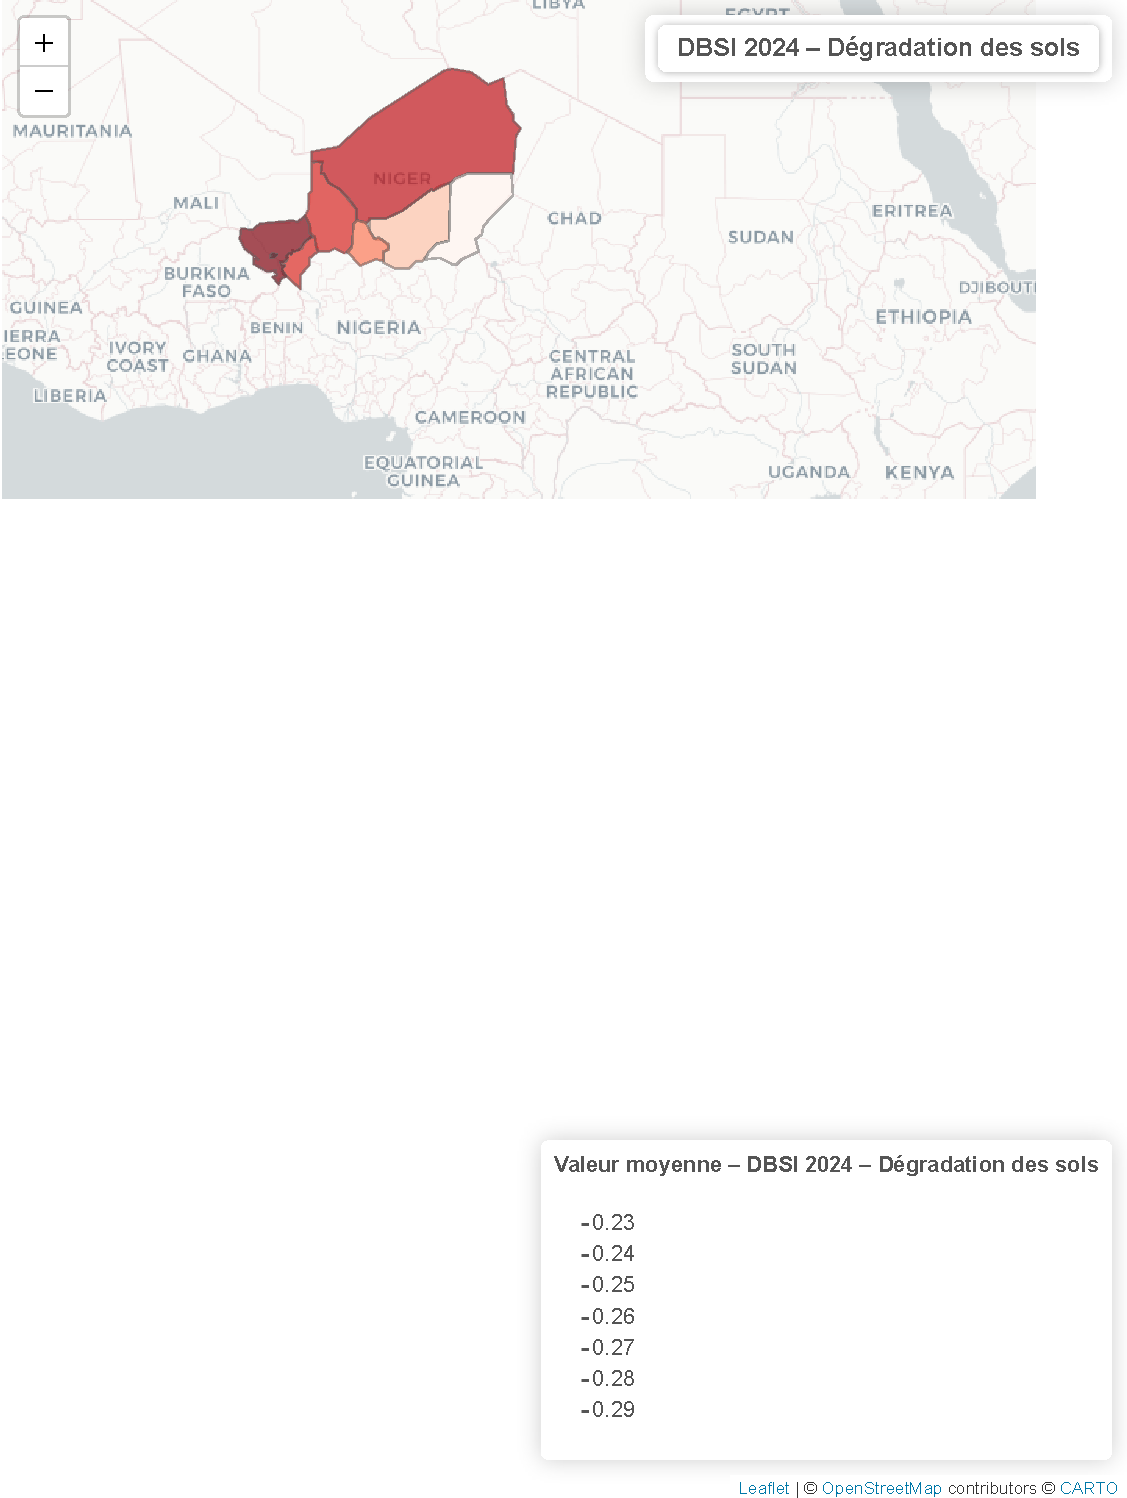
\includegraphics{Atlas-Spectral-Sahel_files/figure-latex/stress-dbsi-1.pdf}

\subsection{Tableau de la répartition du DBSI au Niger en 2024}\label{tableau-de-la-ruxe9partition-du-dbsi-au-niger-en-2024}

\begin{table}[!t]
\caption*{
{\large \textbf{Moyennes régionales du DBSI}} \\ 
{\small \emph{Niger -- Année 2024}}
} 
\fontsize{12.0pt}{14.4pt}\selectfont
\begin{tabular*}{\linewidth}{@{\extracolsep{\fill}}lr}
\toprule
{RÉGION} & {DBSI} \\ 
\midrule\addlinespace[2.5pt]
Zinder & {\cellcolor[HTML]{FDC2AA}{\textcolor[HTML]{000000}{0.238}}} \\ 
Dosso & {\cellcolor[HTML]{DB2A24}{\textcolor[HTML]{FFFFFF}{0.273}}} \\ 
Tillabéri & {\cellcolor[HTML]{810511}{\textcolor[HTML]{FFFFFF}{0.292}}} \\ 
Tahoua & {\cellcolor[HTML]{D72622}{\textcolor[HTML]{FFFFFF}{0.274}}} \\ 
Agadez & {\cellcolor[HTML]{C0151B}{\textcolor[HTML]{FFFFFF}{0.280}}} \\ 
Niamey & {\cellcolor[HTML]{67000D}{\textcolor[HTML]{FFFFFF}{0.296}}} \\ 
Diffa & {\cellcolor[HTML]{FFF5F0}{\textcolor[HTML]{000000}{0.221}}} \\ 
Maradi & {\cellcolor[HTML]{FC7A59}{\textcolor[HTML]{FFFFFF}{0.255}}} \\ 
\bottomrule
\end{tabular*}
\end{table}

\subsection{Analyse des résultats}\label{analyse-des-ruxe9sultats-10}

L'indice \textbf{DBSI} permet d'estimer la \textbf{proportion de sol nu et sec} à la surface, ce qui en fait un excellent indicateur de \textbf{dégradation avancée des terres}, de \textbf{perte de couverture végétale} et de \textbf{fragilité écologique}. Des valeurs plus \textbf{élevées} du DBSI traduisent une \textbf{exposition accrue du sol}, souvent liée à la \textbf{désertification}, à la \textbf{surexploitation agropastorale}, ou à des conditions climatiques extrêmes.

En 2024, les valeurs du DBSI au \textbf{Niger} varient de \textbf{0.221 à 0.296}, avec une tendance généralisée à la \textbf{présence dominante de sols nus dans presque toutes les régions}.

Les \textbf{valeurs les plus élevées} sont observées dans les régions de \textbf{Niamey (0.296)}, \textbf{Tillabéri (0.292)}, et \textbf{Agadez (0.280)}. Ces chiffres reflètent une \textbf{exposition importante du sol}, due soit à une \textbf{urbanisation intense} (Niamey), soit à des \textbf{milieux très arides ou désertiques} (Agadez), ou encore à des pratiques agricoles intensives sans couverture végétale suffisante (Tillabéri). Ces régions peuvent être considérées comme des \textbf{points critiques de dégradation écologique visible}.

Les \textbf{valeurs intermédiaires}, comprises entre \textbf{0.255 et 0.274}, sont relevées dans \textbf{Tahoua (0.274)}, \textbf{Dosso (0.273)}, et \textbf{Maradi (0.255)}. Ces régions du centre-sud du pays connaissent une \textbf{végétation saisonnière fragile} et sont soumises à une \textbf{pression agropastorale croissante}, ce qui entraîne une \textbf{diminution progressive de la couverture végétale} au profit de sols nus ou peu protégés.

Les \textbf{valeurs les plus faibles}, bien qu'encore élevées, concernent \textbf{Zinder (0.238)} et \textbf{Diffa (0.221)}. Cela pourrait s'expliquer par une \textbf{couverture végétale légèrement plus présente} au moment de l'observation satellitaire, ou par des \textbf{caractéristiques de sol spécifiques} (texture, humidité résiduelle) atténuant la réflectance typique des sols nus. Toutefois, ces régions restent dans une \textbf{zone de vigilance élevée}, car même ces ``faibles'' valeurs dépassent les seuils généralement associés à des surfaces stables.

Dans l'ensemble, le \textbf{DBSI confirme une exposition généralisée du sol nu à travers tout le territoire nigérien}, avec des \textbf{poches de dégradation avancée}, en particulier dans l'ouest et le centre du pays. Cette situation renforce l'urgence de mettre en place des \textbf{programmes de reboisement, de gestion anti-érosive et de régénération naturelle assistée}, notamment dans les régions les plus exposées.

\section{Eau et humidité -- WI2}\label{eau-et-humidituxe9-wi2}

Le \textbf{WI2 (Water Index 2)} est un indice spectral conçu pour détecter la \textbf{présence d'eau ou d'humidité de surface}, même en très faibles quantités. Il repose sur une combinaison des bandes \textbf{NIR (infrarouge proche)} et \textbf{SWIR (infrarouge moyen)}, qui sont sensibles à la \textbf{teneur en eau des sols} et des surfaces végétales.

Le WI2 est particulièrement utile dans les \textbf{milieux semi-arides et sahéliens}, comme ceux du \textbf{Niger}, où l'humidité est rare, diffuse, et difficile à détecter. Il permet d'identifier les \textbf{zones humides résiduelles}, les \textbf{vallées fluviales}, les \textbf{mares temporaires}, ou les \textbf{bas-fonds agricoles} présentant encore une capacité de rétention d'eau.

Contrairement aux indices végétatifs classiques, le WI2 ne se limite pas à la végétation : il mesure directement les \textbf{contrastes d'absorption de l'eau} dans le spectre infrarouge, ce qui en fait un outil précieux pour le \textbf{suivi hydrologique}, la \textbf{gestion des terres agricoles}, et la \textbf{prévision des déficits hydriques}.

Dans le cas du \textbf{Niger}, les \textbf{valeurs moyennes du WI2 pour l'année 2024} ont été extraites à partir d'images satellites haute résolution, puis \textbf{agrégées par région administrative}. Cette analyse permet de mettre en évidence les \textbf{régions disposant encore d'humidité résiduelle}, et celles déjà en \textbf{situation de stress hydrique sévère}.

\begin{center}\rule{0.5\linewidth}{0.5pt}\end{center}

\subsection{Carte interactive du WI2 au Niger en 2024}\label{carte-interactive-du-wi2-au-niger-en-2024}

\begin{verbatim}
##   |                                                                              |                                                                      |   0%  |                                                                              |=========                                                             |  12%  |                                                                              |==================                                                    |  25%  |                                                                              |==========================                                            |  38%  |                                                                              |===================================                                   |  50%  |                                                                              |============================================                          |  62%  |                                                                              |====================================================                  |  75%  |                                                                              |=============================================================         |  88%  |                                                                              |======================================================================| 100%
\end{verbatim}

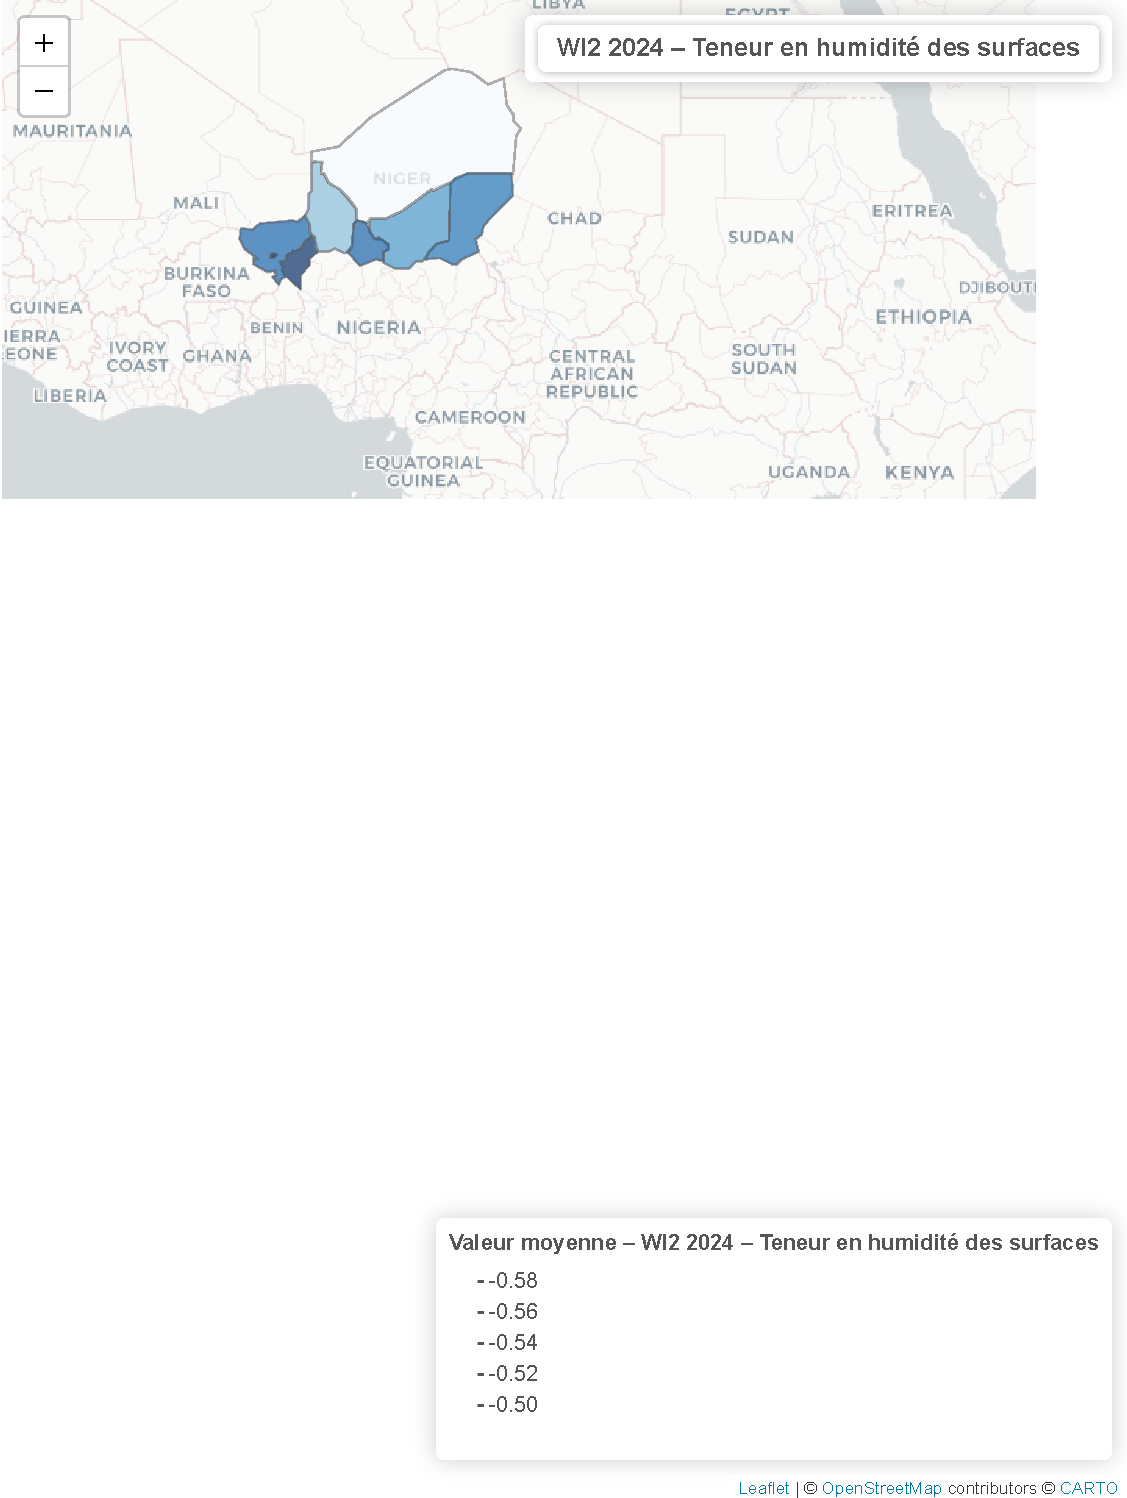
\includegraphics{Atlas-Spectral-Sahel_files/figure-latex/eau-wi2-1.pdf}

\begin{center}\rule{0.5\linewidth}{0.5pt}\end{center}

\subsection{Tableau de la répartition du WI2 au Niger en 2024}\label{tableau-de-la-ruxe9partition-du-wi2-au-niger-en-2024}

\begin{table}[!t]
\caption*{
{\large \textbf{Moyennes régionales du WI2}} \\ 
{\small \emph{Niger -- Année 2024}}
} 
\fontsize{12.0pt}{14.4pt}\selectfont
\begin{tabular*}{\linewidth}{@{\extracolsep{\fill}}lr}
\toprule
{RÉGION} & {WI2} \\ 
\midrule\addlinespace[2.5pt]
Zinder & {\cellcolor[HTML]{4B98C9}{\textcolor[HTML]{FFFFFF}{-0.525}}} \\ 
Dosso & {\cellcolor[HTML]{08306B}{\textcolor[HTML]{FFFFFF}{-0.485}}} \\ 
Tillabéri & {\cellcolor[HTML]{1B67AD}{\textcolor[HTML]{FFFFFF}{-0.506}}} \\ 
Tahoua & {\cellcolor[HTML]{89BEDC}{\textcolor[HTML]{000000}{-0.542}}} \\ 
Agadez & {\cellcolor[HTML]{F7FBFF}{\textcolor[HTML]{000000}{-0.585}}} \\ 
Niamey & {\cellcolor[HTML]{094286}{\textcolor[HTML]{FFFFFF}{-0.492}}} \\ 
Diffa & {\cellcolor[HTML]{2474B6}{\textcolor[HTML]{FFFFFF}{-0.511}}} \\ 
Maradi & {\cellcolor[HTML]{1964AB}{\textcolor[HTML]{FFFFFF}{-0.505}}} \\ 
\bottomrule
\end{tabular*}
\end{table}

\begin{center}\rule{0.5\linewidth}{0.5pt}\end{center}

\subsection{Analyse des résultats}\label{analyse-des-ruxe9sultats-11}

L'indice \textbf{WI2} permet de mesurer la \textbf{teneur en humidité de surface}, qu'il s'agisse d'eau libre, d'humidité des sols ou de traces hydriques résiduelles. Des valeurs \textbf{plus proches de zéro} indiquent une \textbf{meilleure humidité}, tandis que des valeurs \textbf{plus négatives} traduisent une \textbf{situation hydrique plus critique}, caractéristique de milieux très secs.

En 2024, les valeurs du WI2 au \textbf{Niger} varient entre \textbf{--0.485 et --0.585}, traduisant une \textbf{situation hydrique globalement préoccupante sur l'ensemble du territoire}, avec des différences subtiles mais significatives entre les régions.

Les \textbf{valeurs les moins négatives}, donc les plus ``humides'' relativement parlant, sont enregistrées dans les régions :
- \textbf{Dosso (--0.485)},
- \textbf{Niamey (--0.492)}.

Ces régions se situent dans le \textbf{sud-ouest du pays}, où la pluviométrie est légèrement plus élevée, et où l'on retrouve des \textbf{zones irriguées}, des \textbf{cours d'eau permanents} comme le fleuve Niger, ainsi qu'une \textbf{activité agricole structurée}. Cette situation suggère une \textbf{humidité résiduelle encore observable}, en dépit des conditions climatiques difficiles.

Les \textbf{valeurs intermédiaires}, autour de \textbf{--0.505 à --0.525}, concernent les régions de \textbf{Zinder}, \textbf{Tillabéri}, \textbf{Maradi} et \textbf{Diffa}. Ces zones connaissent une \textbf{saison humide courte}, suivie d'une \textbf{évaporation rapide}, ce qui engendre une humidité de surface très limitée en dehors des périodes de pluie. Les valeurs observées traduisent un \textbf{équilibre fragile}, où l'humidité disponible ne permet qu'une \textbf{végétation saisonnière temporaire}.

La région la plus sèche selon le WI2 est \textbf{Agadez (--0.585)}, suivie de \textbf{Tahoua (--0.542)}. Ces résultats sont cohérents avec la \textbf{domination saharienne et sub-saharienne} de ces zones, où les \textbf{sources d'humidité sont extrêmement rares}, les \textbf{sols très perméables}, et la \textbf{végétation quasi absente}. Ces régions cumulent les \textbf{conditions hydriques les plus défavorables} du pays.

Globalement, cette cartographie du WI2 met en évidence une \textbf{teneur en eau de surface extrêmement faible dans l'ensemble du territoire nigérien}, confirmant la \textbf{sécheresse structurelle} du pays. Elle souligne l'importance de stratégies d'\textbf{adaptation hydrique}, de \textbf{gestion de l'eau agricole}, et de \textbf{surveillance spatialisée de l'humidité}, pour anticiper les \textbf{crises agro-hydrologiques} dans un contexte de changement climatique.

\begin{center}\rule{0.5\linewidth}{0.5pt}\end{center}

\section{Conclusion}\label{conclusion-3}

L'analyse conjointe des indices \textbf{ATSAVI}, \textbf{DBSI} et \textbf{WI2} offre une lecture nuancée et spatialement explicite de l'\textbf{état environnemental du Niger en 2024}. Dans un pays marqué par l'aridité, la fragilité des écosystèmes et la pression climatique, ces indicateurs révèlent des dynamiques contrastées entre \textbf{résilience végétale localisée}, \textbf{dégradation diffuse} et \textbf{raréfaction de l'humidité de surface}.

L'\textbf{ATSAVI} met en lumière une \textbf{couverture végétale extrêmement faible}, concentrée dans les régions méridionales comme \textbf{Dosso} ou \textbf{Maradi}, où la végétation subsiste sous forme saisonnière, souvent liée à des activités agricoles localisées. Le reste du territoire montre une \textbf{végétation quasi absente}, conséquence directe de l'aridité structurelle et des pressions environnementales.

Le \textbf{DBSI} confirme cette dégradation, avec des niveaux élevés de \textbf{sols nus et secs} dans presque toutes les régions. Des zones comme \textbf{Niamey}, \textbf{Tillabéri} ou \textbf{Agadez} affichent une exposition avancée des sols, symptôme de \textbf{surexploitation}, de \textbf{déforestation}, ou d'une \textbf{perte progressive de couverture protectrice}, accentuant les risques d'érosion et d'insécurité écologique.

Enfin, le \textbf{WI2} indique une \textbf{teneur en humidité de surface extrêmement faible} dans l'ensemble du pays, avec des conditions hydriques particulièrement critiques dans des régions comme \textbf{Agadez} et \textbf{Tahoua}. Même dans les zones plus favorisées du sud-ouest, l'humidité reste marginale, renforçant la \textbf{vulnérabilité hydrique structurelle} du Niger.

Ce chapitre met ainsi en évidence la \textbf{nécessité d'interventions ciblées} en matière de \textbf{reboisement, de sécurisation des sols, de gestion hydrique et d'agriculture résiliente}. Face aux défis combinés du climat, de la pression démographique et de la dégradation écologique, le suivi régulier de ces indicateurs apparaît comme un outil essentiel pour éclairer les décisions politiques et renforcer la \textbf{résilience des territoires}.

\begin{center}\rule{0.5\linewidth}{0.5pt}\end{center}

\begin{quote}
\emph{« Là où la pluie devient mémoire, l'avenir se dessine dans l'économie de chaque goutte. »}\\
--- \textbf{Issoufou Mahamadou}
\end{quote}

\chapter{Exploration des indicateurs}\label{exploration-des-indicateurs}

\section{Introduction}\label{introduction-4}

L'objectif de ce chapitre est de comparer les dynamiques environnementales entre les quatre pays étudiés --- \textbf{Sénégal}, \textbf{Burkina Faso}, \textbf{Mali} et \textbf{Niger} --- à partir d'une sélection d'\textbf{indicateurs spectraux homogènes}, calculés sur l'ensemble du territoire national de chaque pays à l'échelle régionale.

Contrairement aux chapitres précédents qui abordaient chaque pays individuellement, l'approche ici est \textbf{transversale} : elle vise à identifier les \textbf{points communs}, les \textbf{disparités}, et les \textbf{profils écologiques contrastés} à travers l'espace sahélien ouest-africain.

Nous nous focalisons sur trois dimensions fondamentales :

\begin{itemize}
\tightlist
\item
  \textbf{La vigueur de la végétation} à travers l'indice \textbf{NDVI} (Normalized Difference Vegetation Index), indicateur standard de la couverture végétale active ;
\item
  \textbf{Le stress ou la dégradation écologique} via le \textbf{BAI} (Burned Area Index), utilisé comme proxy de la perturbation de surface (sols nus, végétation appauvrie, zones brûlées) ;
\item
  \textbf{L'humidité résiduelle des surfaces} à travers l'indice \textbf{WI2} (Water Index 2), mesurant la présence d'eau ou d'humidité dans le sol et la végétation.
\end{itemize}

Pour chaque indicateur, nous présentons :

\begin{itemize}
\tightlist
\item
  Des \textbf{cartes par pays},
\item
  Un \textbf{graphique comparatif} des moyennes nationales,
\item
  Un \textbf{tableau régional détaillé} des valeurs.
\end{itemize}

Cette démarche permet d'établir un \textbf{diagnostic spatial comparé}, et d'alimenter une réflexion plus large sur la résilience écologique, les pressions climatiques et les marges d'action pour une gestion durable des ressources naturelles à l'échelle régionale.

\begin{center}\rule{0.5\linewidth}{0.5pt}\end{center}

\section{Introduction}\label{introduction-5}

L'objectif de ce chapitre est de comparer les dynamiques environnementales entre les quatre pays étudiés --- \textbf{Sénégal}, \textbf{Burkina Faso}, \textbf{Mali} et \textbf{Niger} --- à partir d'une sélection d'\textbf{indicateurs spectraux homogènes}, calculés sur l'ensemble du territoire national de chaque pays à l'échelle régionale.

Contrairement aux chapitres précédents qui abordaient chaque pays individuellement, l'approche ici est \textbf{transversale} : elle vise à identifier les \textbf{points communs}, les \textbf{disparités}, et les \textbf{profils écologiques contrastés} à travers l'espace sahélien ouest-africain.

Nous nous focalisons sur trois dimensions fondamentales :

\begin{itemize}
\tightlist
\item
  \textbf{La vigueur de la végétation} à travers l'indice \textbf{NDVI} (Normalized Difference Vegetation Index), indicateur standard de la couverture végétale active ;
\item
  \textbf{Le stress ou la dégradation écologique} via le \textbf{BAI} (Burned Area Index), utilisé comme proxy de la perturbation de surface (sols nus, végétation appauvrie, zones brûlées) ;
\item
  \textbf{L'humidité résiduelle des surfaces} à travers l'indice \textbf{WI2} (Water Index 2), mesurant la présence d'eau ou d'humidité dans le sol et la végétation.
\end{itemize}

Pour chaque indicateur, nous présentons :

\begin{itemize}
\tightlist
\item
  Des \textbf{cartes par pays},
\item
  Un \textbf{graphique comparatif} des moyennes nationales,
\item
  Un \textbf{tableau régional détaillé} des valeurs.
\end{itemize}

Cette démarche permet d'établir un \textbf{diagnostic spatial comparé}, et d'alimenter une réflexion plus large sur la résilience écologique, les pressions climatiques et les marges d'action pour une gestion durable des ressources naturelles à l'échelle régionale.

\section{Comparaison de la couverture végétale}\label{comparaison-de-la-couverture-vuxe9guxe9tale}

L'indice NDVI (Normalized Difference Vegetation Index) est un indicateur standard de la densité de la végétation verte active. Il permet d'observer les zones à fort potentiel de biomasse ainsi que les zones dégradées. Dans ce cadre comparatif, nous utilisons le NDVI pour analyser les différences de couverture végétale entre les pays sahéliens.

\subsection{Cartes NDVI par pays}\label{cartes-ndvi-par-pays}

\begin{verbatim}
##   |                                                                              |                                                                      |   0%  |                                                                              |=====                                                                 |   7%  |                                                                              |==========                                                            |  14%  |                                                                              |===============                                                       |  21%  |                                                                              |====================                                                  |  29%  |                                                                              |=========================                                             |  36%  |                                                                              |==============================                                        |  43%  |                                                                              |===================================                                   |  50%  |                                                                              |========================================                              |  57%  |                                                                              |=============================================                         |  64%  |                                                                              |==================================================                    |  71%  |                                                                              |=======================================================               |  79%  |                                                                              |============================================================          |  86%  |                                                                              |=================================================================     |  93%  |                                                                              |======================================================================| 100%
\end{verbatim}

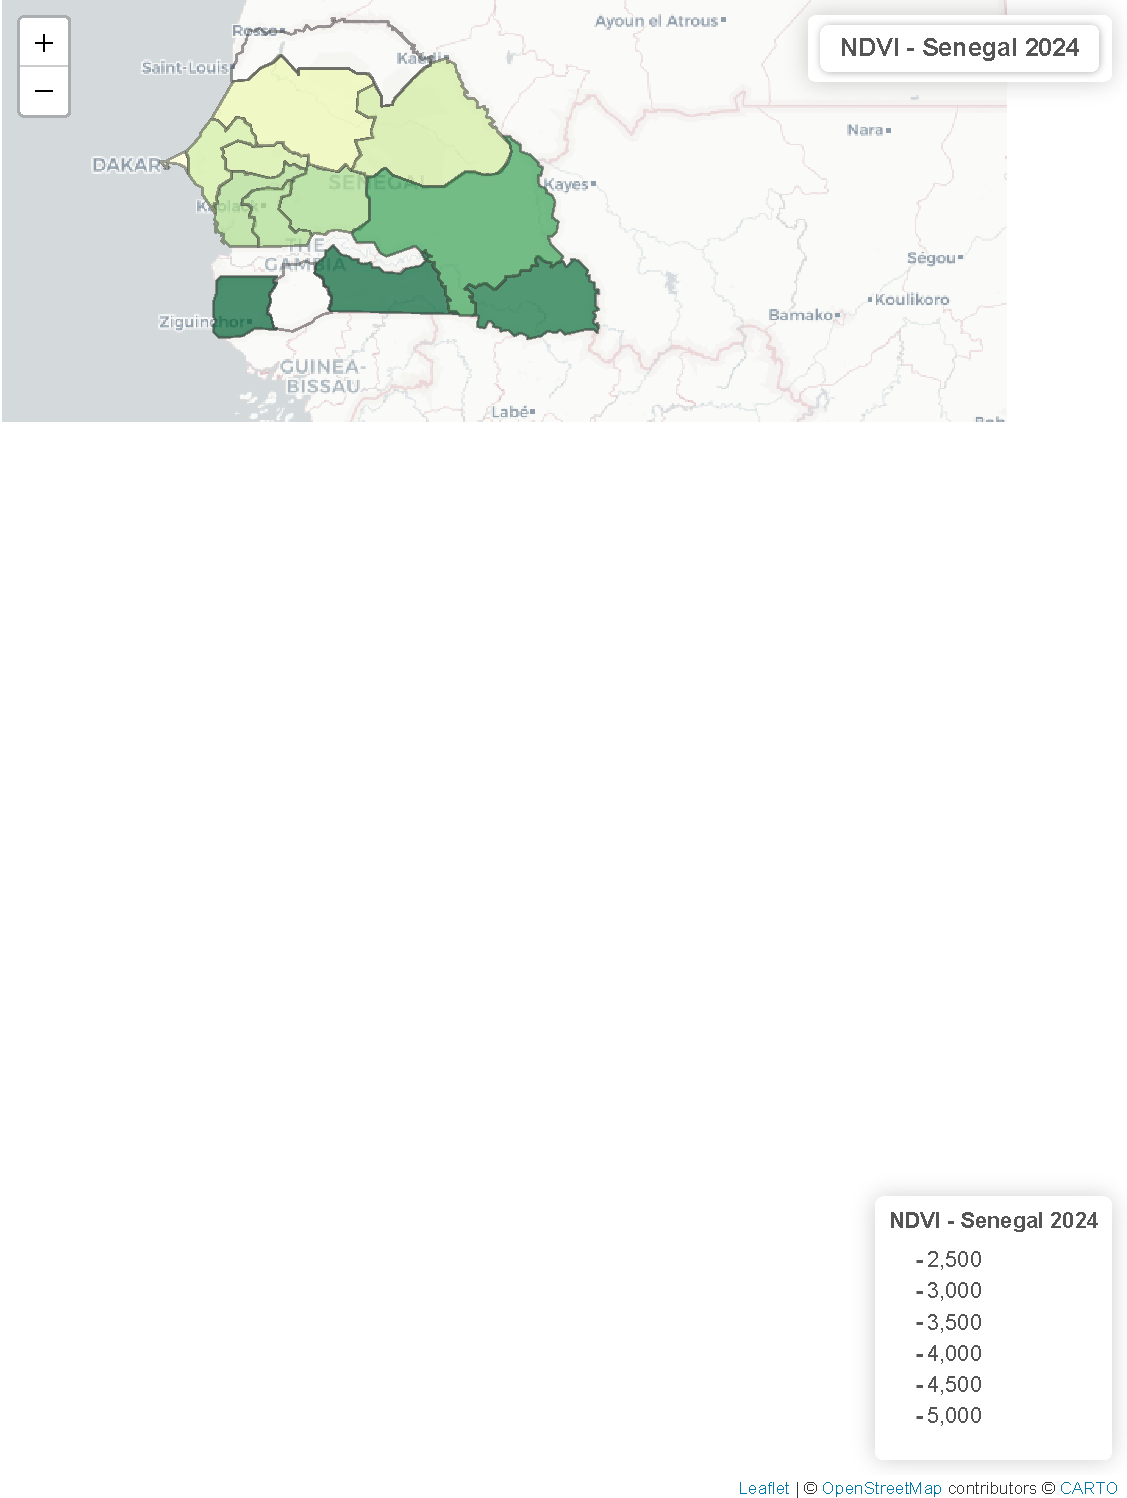
\includegraphics{Atlas-Spectral-Sahel_files/figure-latex/ndvi-cartes-1.pdf}

\begin{verbatim}
##   |                                                                              |                                                                      |   0%  |                                                                              |=====                                                                 |   8%  |                                                                              |===========                                                           |  15%  |                                                                              |================                                                      |  23%  |                                                                              |======================                                                |  31%  |                                                                              |===========================                                           |  38%  |                                                                              |================================                                      |  46%  |                                                                              |======================================                                |  54%  |                                                                              |===========================================                           |  62%  |                                                                              |================================================                      |  69%  |                                                                              |======================================================                |  77%  |                                                                              |===========================================================           |  85%  |                                                                              |=================================================================     |  92%  |                                                                              |======================================================================| 100%
\end{verbatim}

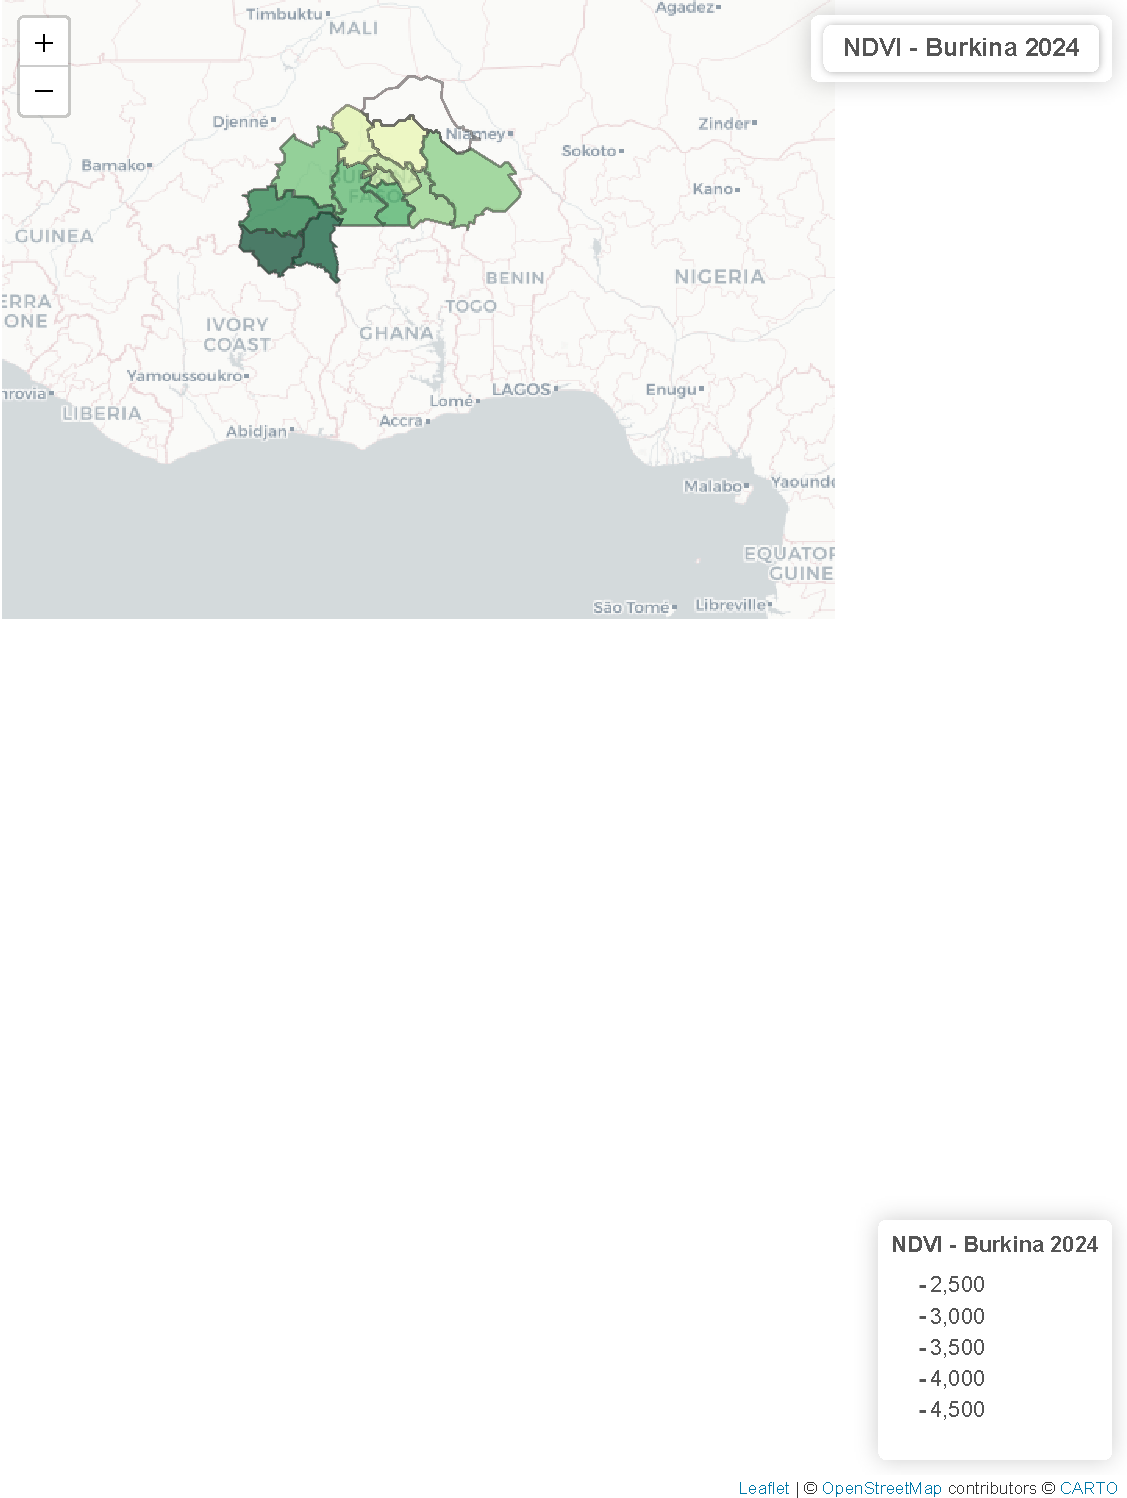
\includegraphics{Atlas-Spectral-Sahel_files/figure-latex/ndvi-cartes-2.pdf}

\begin{verbatim}
##   |                                                                              |                                                                      |   0%  |                                                                              |=======                                                               |  10%  |                                                                              |==============                                                        |  20%  |                                                                              |=====================                                                 |  30%  |                                                                              |============================                                          |  40%  |                                                                              |===================================                                   |  50%  |                                                                              |==========================================                            |  60%  |                                                                              |=================================================                     |  70%  |                                                                              |========================================================              |  80%  |                                                                              |===============================================================       |  90%  |                                                                              |======================================================================| 100%
\end{verbatim}

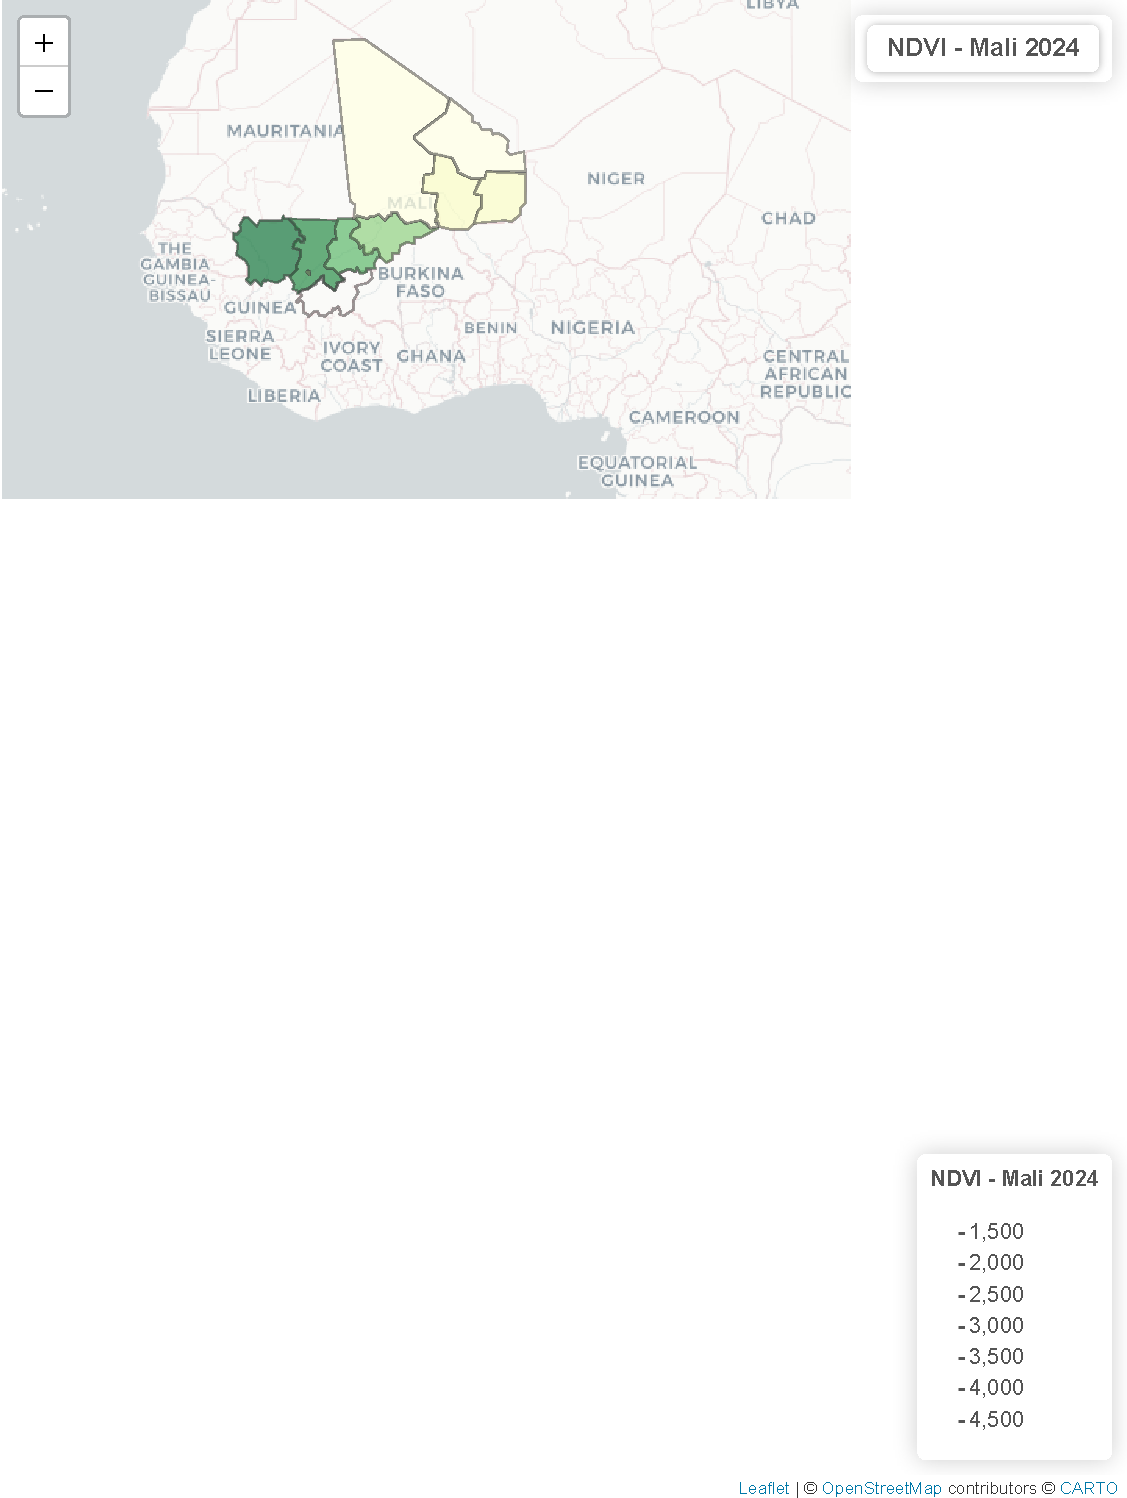
\includegraphics{Atlas-Spectral-Sahel_files/figure-latex/ndvi-cartes-3.pdf}

\begin{verbatim}
##   |                                                                              |                                                                      |   0%  |                                                                              |=========                                                             |  12%  |                                                                              |==================                                                    |  25%  |                                                                              |==========================                                            |  38%  |                                                                              |===================================                                   |  50%  |                                                                              |============================================                          |  62%  |                                                                              |====================================================                  |  75%  |                                                                              |=============================================================         |  88%  |                                                                              |======================================================================| 100%
\end{verbatim}

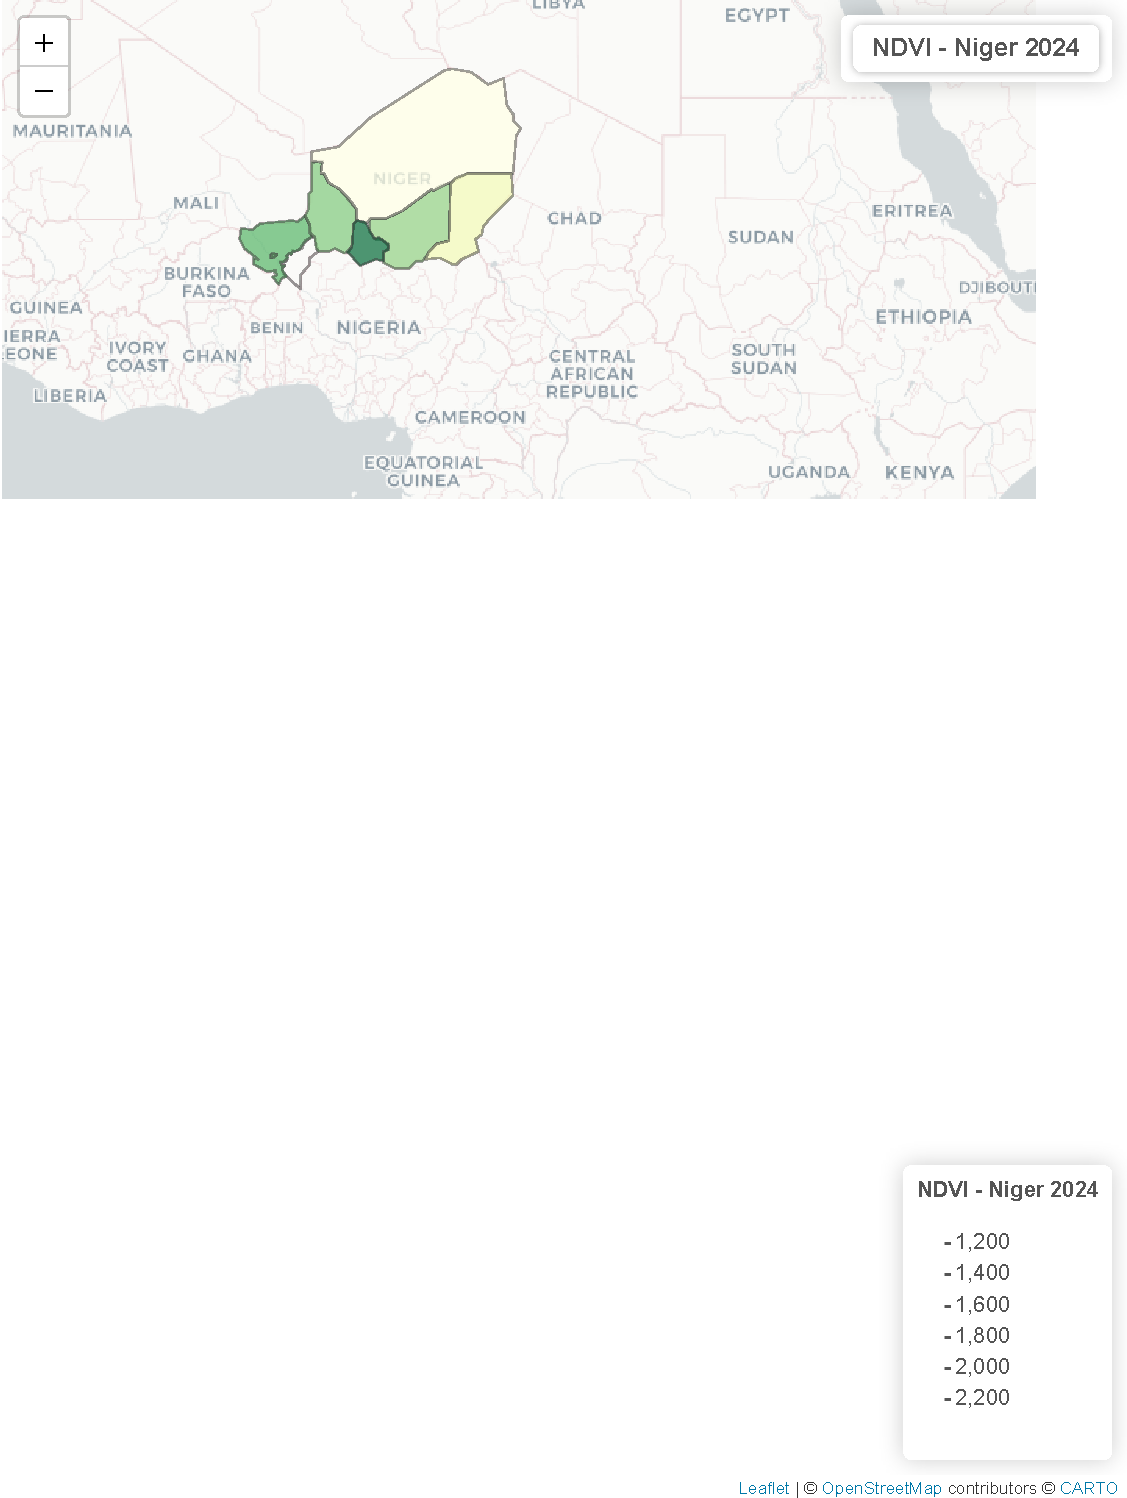
\includegraphics{Atlas-Spectral-Sahel_files/figure-latex/ndvi-cartes-4.pdf}
\#\#\# Moyenne NDVI par pays
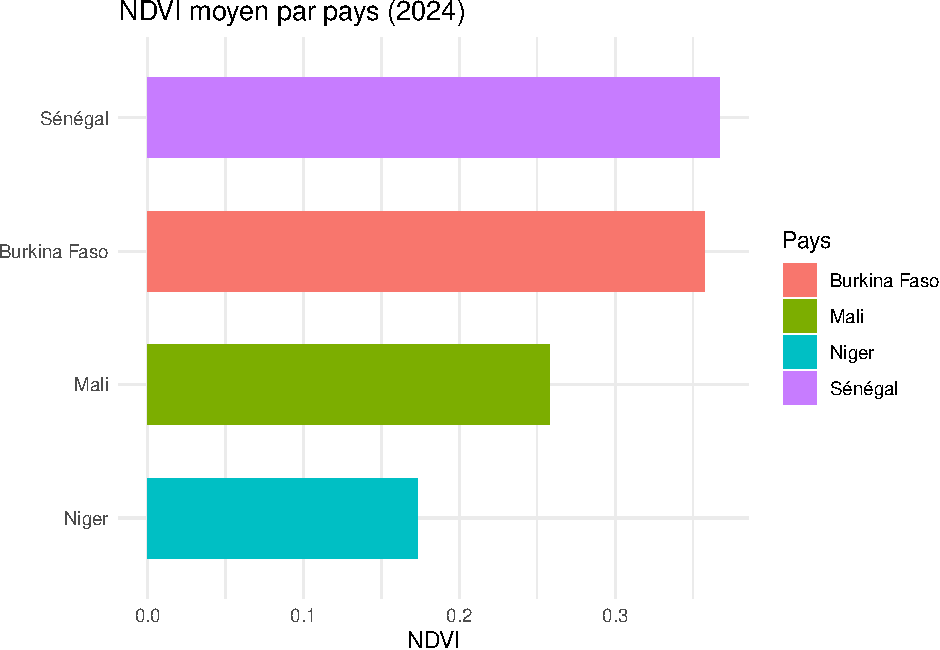
\includegraphics{Atlas-Spectral-Sahel_files/figure-latex/ndvi-plot-1.pdf}

\subsection{Tableau des valeurs régionales NDVI}\label{tableau-des-valeurs-ruxe9gionales-ndvi}

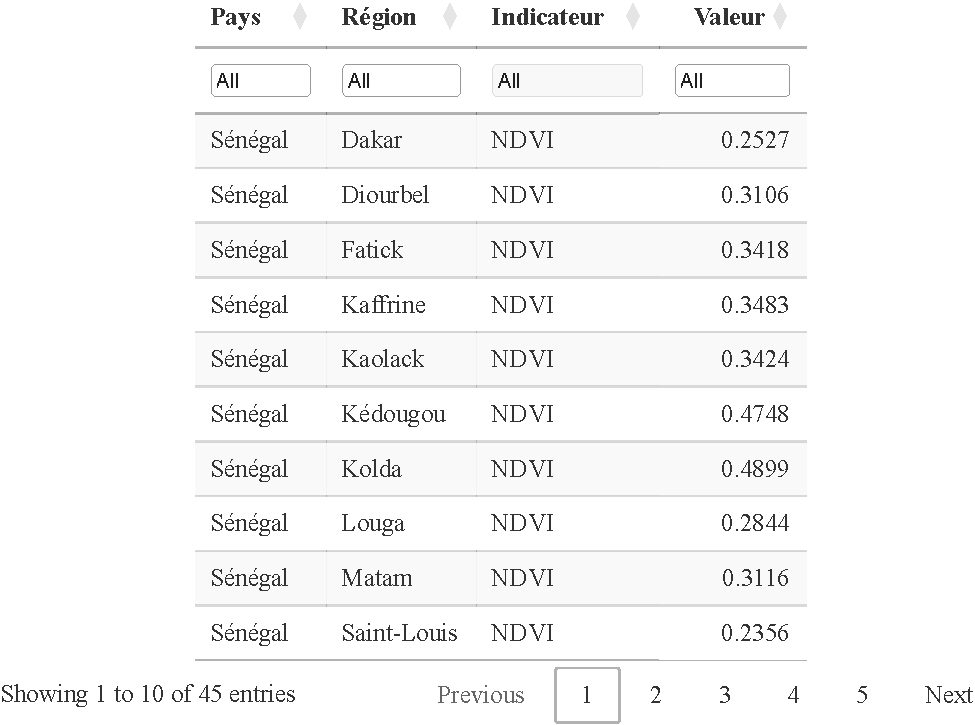
\includegraphics{Atlas-Spectral-Sahel_files/figure-latex/ndvi-table-1.pdf}

\subsection{Analyse comparative}\label{analyse-comparative}

Le \textbf{NDVI (Normalized Difference Vegetation Index)} est un indicateur de référence pour estimer la \textbf{densité de végétation active} à la surface terrestre. Calculé à partir des bandes rouge et proche infrarouge des satellites, il permet de quantifier la \textbf{vigueur photosynthétique des plantes}. Plus la valeur est élevée, plus la couverture végétale est dense, verte et en bonne santé.

\begin{center}\rule{0.5\linewidth}{0.5pt}\end{center}

\subsubsection{Lecture interne (intra-pays)}\label{lecture-interne-intra-pays}

Dans chacun des pays sahéliens étudiés (🇸🇳 Sénégal, 🇧🇫 Burkina Faso, 🇲🇱 Mali, 🇳🇪 Niger), on observe un \textbf{gradient écologique du nord vers le sud} :

\begin{itemize}
\tightlist
\item
  \textbf{Au nord} : zones sahéliennes, plus sèches, avec une végétation clairsemée voire absente.
\item
  \textbf{Au sud} : zones soudaniennes ou guinéennes, plus humides, avec forêts, savanes denses et cultures.
\end{itemize}

Cette dynamique se vérifie dans chaque territoire :

\begin{itemize}
\tightlist
\item
  \textbf{Sénégal} : NDVI élevé au sud (Ziguinchor, Sédhiou, Kolda), plus faible au nord (Matam, Saint-Louis).
\item
  \textbf{Mali} : végétation dense au sud (Sikasso), quasi absente au nord (Kidal, Tombouctou).
\item
  \textbf{Burkina Faso} : valeurs plus élevées dans le Sud-Ouest et les Cascades, plus faibles dans le Sahel burkinabè.
\item
  \textbf{Niger} : contraste extrême entre les régions méridionales (Maradi, Dosso) et les étendues désertiques du nord (Agadez).
\end{itemize}

\begin{quote}
\textbf{Conclusion intra-pays} : dans chacun des pays étudiés, \textbf{la végétation devient plus abondante et plus vigoureuse à mesure qu'on se dirige vers le sud}, conformément à la distribution des précipitations et des biomes.
\end{quote}

\begin{center}\rule{0.5\linewidth}{0.5pt}\end{center}

\subsubsection{Lecture externe (inter-pays)}\label{lecture-externe-inter-pays}

Le graphique comparatif inter-pays révèle des écarts significatifs :

\begin{itemize}
\tightlist
\item
  \textbf{Sénégal} : NDVI moyen le plus élevé, en raison de la forte végétation au sud-ouest (forêts galeries, bolongs, agriculture pluviale).
\item
  \textbf{Burkina Faso} : NDVI stable, reflétant un territoire écologiquement diversifié, bien que soumis à des pressions croissantes.
\item
  \textbf{Mali} : NDVI intermédiaire, marqué par une hétérogénéité importante entre le sud et les zones désertiques.
\item
  \textbf{Niger} : NDVI le plus faible, témoignant d'un territoire très aride avec une végétation clairsemée, voire inexistante dans certaines régions.
\end{itemize}

Le \textbf{Sénégal} et le \textbf{Burkina Faso} apparaissent comme les pays les plus végétalisés en moyenne, tandis que le \textbf{Niger reste le plus vulnérable à la désertification}.

\begin{center}\rule{0.5\linewidth}{0.5pt}\end{center}

\section{5.3 Comparaison du stress écologique}\label{comparaison-du-stress-uxe9cologique}

L'indice BAI (Burned Area Index) est conçu pour détecter les zones brûlées ou fortement dégradées, en mettant en évidence les sols sombres, nus ou perturbés. Bien qu'initialement utilisé pour cartographier les feux de végétation, le BAI est aussi un indicateur pertinent du stress écologique dans les environnements sahéliens, où il révèle les zones de déforestation, surpâturage, sécheresse prolongée ou dégradation des sols.

\subsection{Cartes BAI par pays}\label{cartes-bai-par-pays}

\begin{verbatim}
##   |                                                                              |                                                                      |   0%  |                                                                              |=====                                                                 |   7%  |                                                                              |==========                                                            |  14%  |                                                                              |===============                                                       |  21%  |                                                                              |====================                                                  |  29%  |                                                                              |=========================                                             |  36%  |                                                                              |==============================                                        |  43%  |                                                                              |===================================                                   |  50%  |                                                                              |========================================                              |  57%  |                                                                              |=============================================                         |  64%  |                                                                              |==================================================                    |  71%  |                                                                              |=======================================================               |  79%  |                                                                              |============================================================          |  86%  |                                                                              |=================================================================     |  93%  |                                                                              |======================================================================| 100%
\end{verbatim}

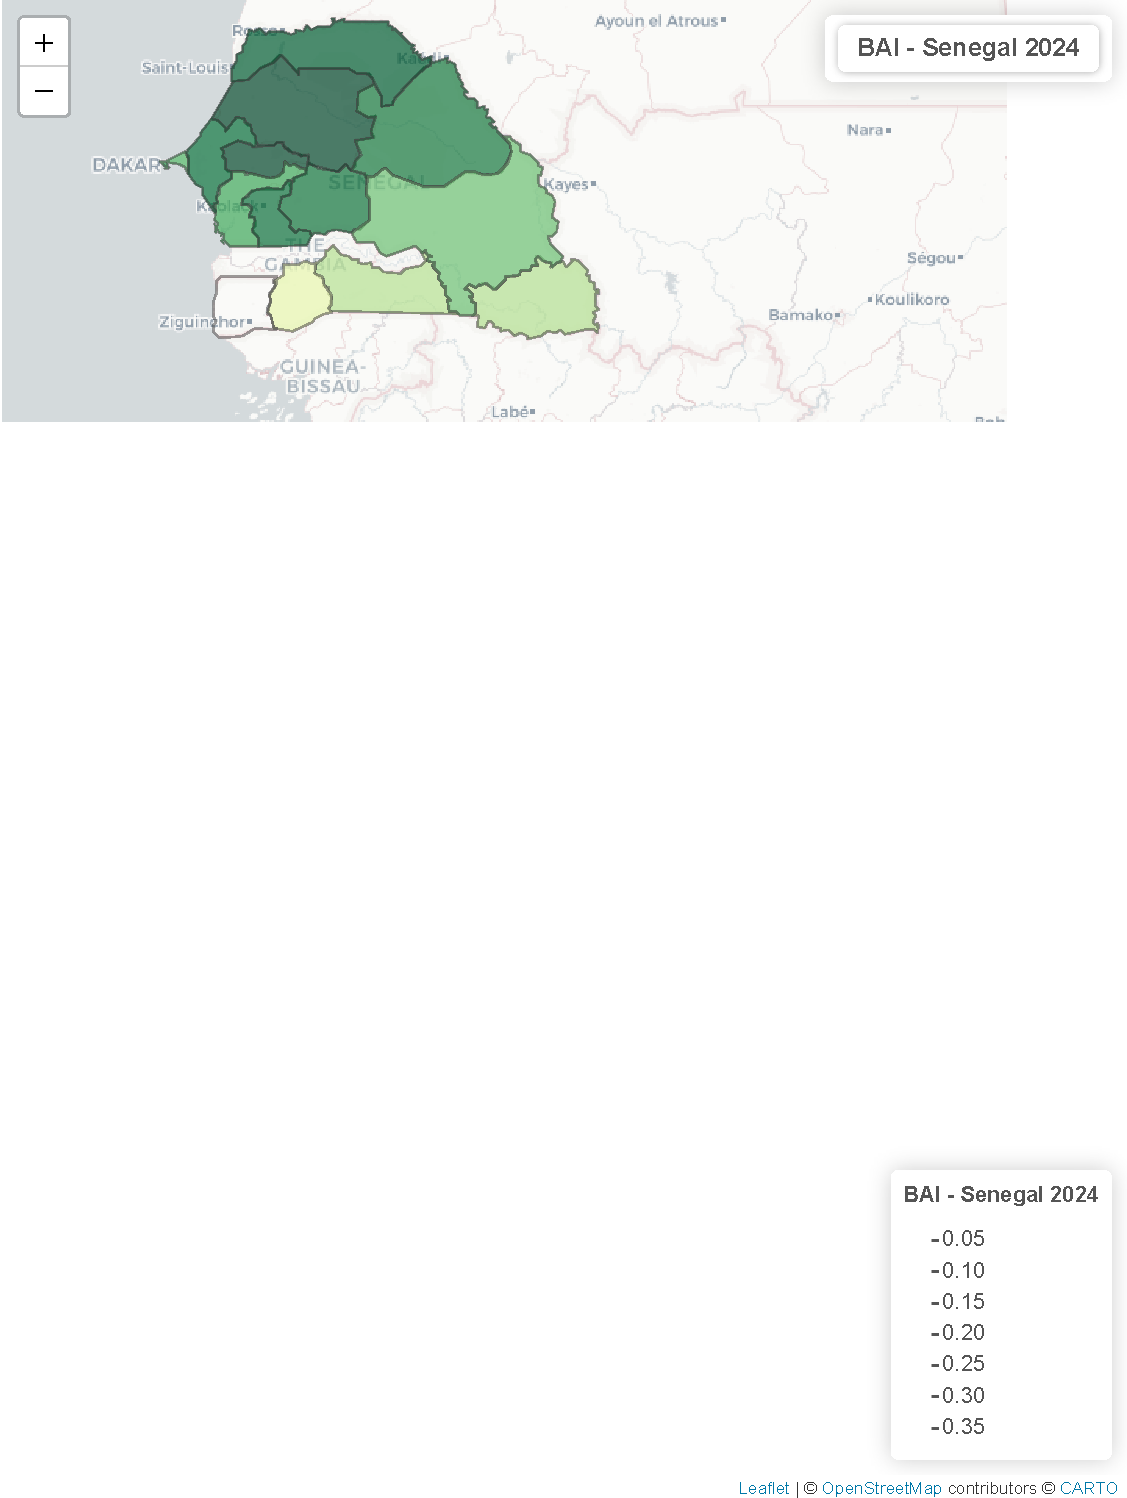
\includegraphics{Atlas-Spectral-Sahel_files/figure-latex/bai-cartes-1.pdf}

\begin{verbatim}
##   |                                                                              |                                                                      |   0%  |                                                                              |=====                                                                 |   8%  |                                                                              |===========                                                           |  15%  |                                                                              |================                                                      |  23%  |                                                                              |======================                                                |  31%  |                                                                              |===========================                                           |  38%  |                                                                              |================================                                      |  46%  |                                                                              |======================================                                |  54%  |                                                                              |===========================================                           |  62%  |                                                                              |================================================                      |  69%  |                                                                              |======================================================                |  77%  |                                                                              |===========================================================           |  85%  |                                                                              |=================================================================     |  92%  |                                                                              |======================================================================| 100%
\end{verbatim}

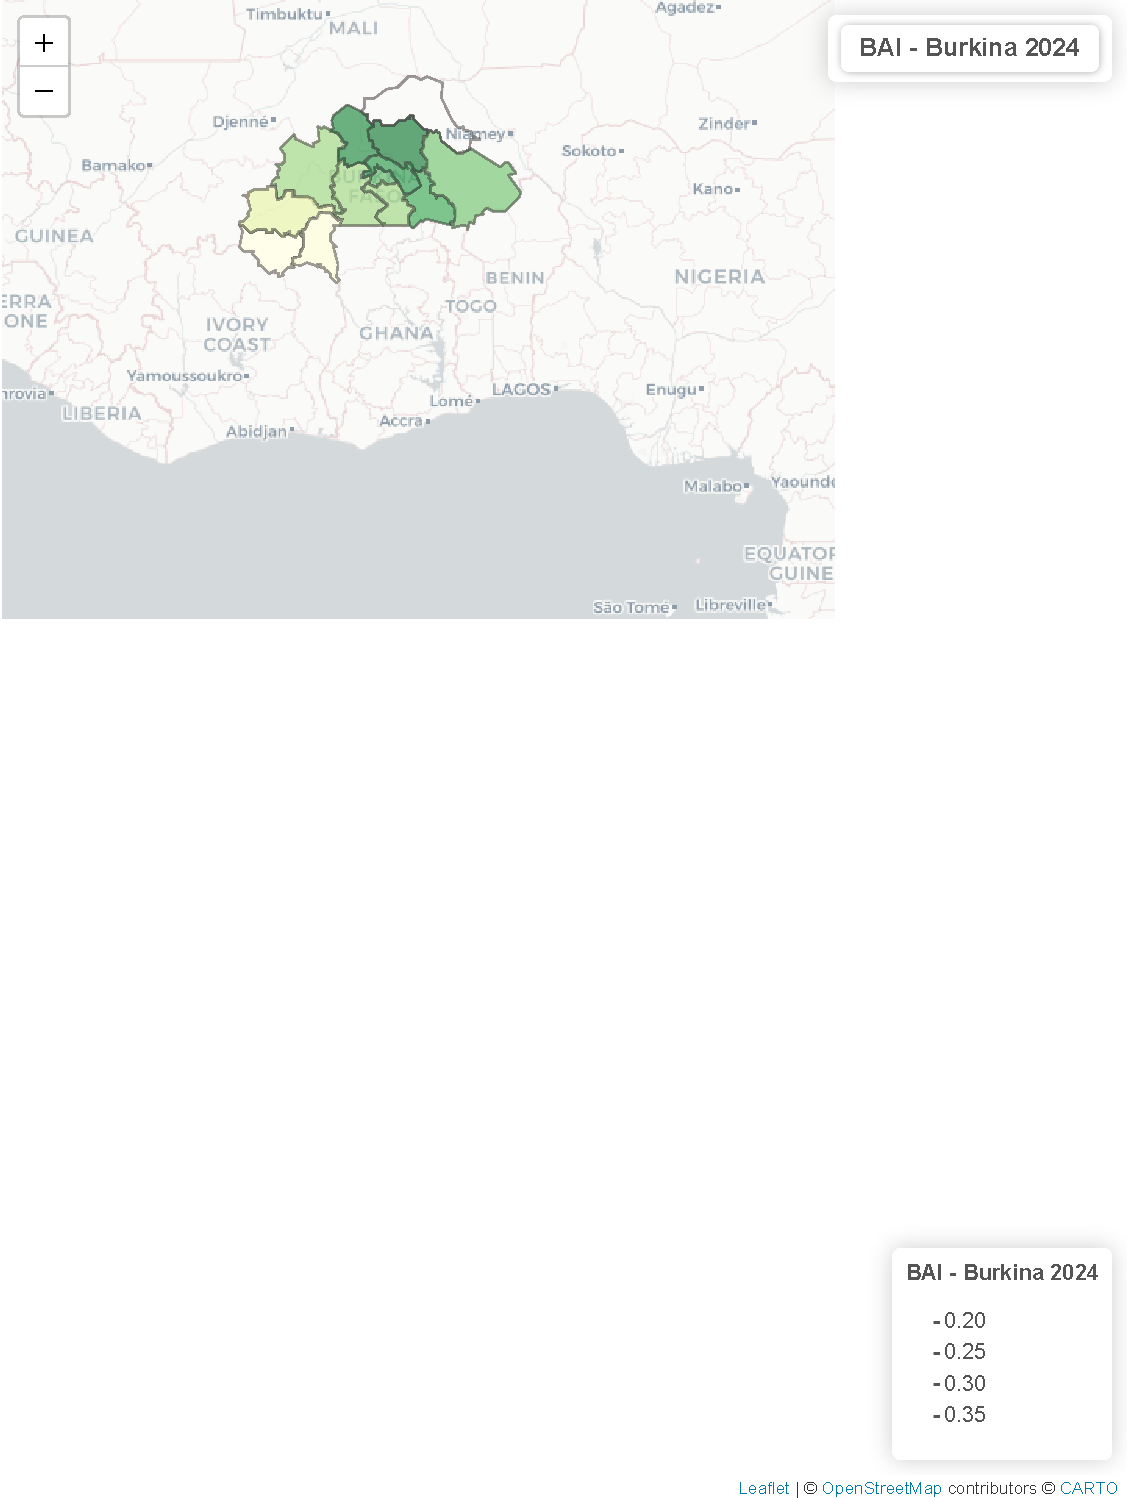
\includegraphics{Atlas-Spectral-Sahel_files/figure-latex/bai-cartes-2.pdf}

\begin{verbatim}
##   |                                                                              |                                                                      |   0%  |                                                                              |=======                                                               |  10%  |                                                                              |==============                                                        |  20%  |                                                                              |=====================                                                 |  30%  |                                                                              |============================                                          |  40%  |                                                                              |===================================                                   |  50%  |                                                                              |==========================================                            |  60%  |                                                                              |=================================================                     |  70%  |                                                                              |========================================================              |  80%  |                                                                              |===============================================================       |  90%  |                                                                              |======================================================================| 100%
\end{verbatim}

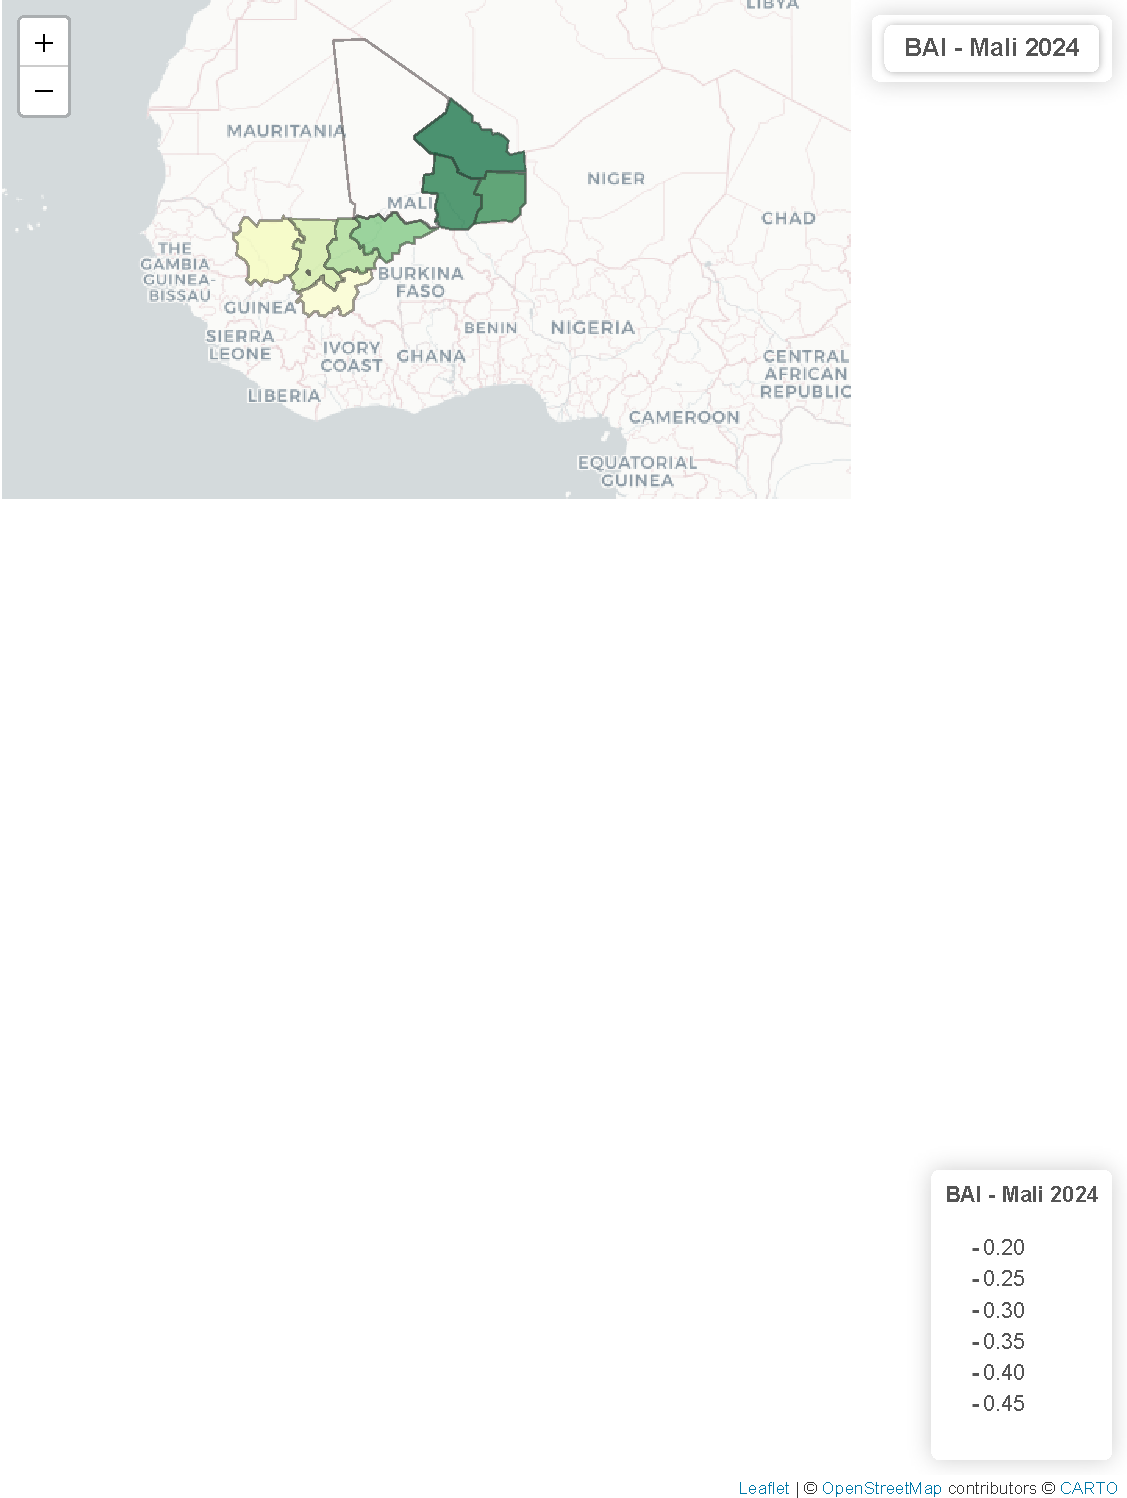
\includegraphics{Atlas-Spectral-Sahel_files/figure-latex/bai-cartes-3.pdf}

\begin{verbatim}
##   |                                                                              |                                                                      |   0%  |                                                                              |=========                                                             |  12%  |                                                                              |==================                                                    |  25%  |                                                                              |==========================                                            |  38%  |                                                                              |===================================                                   |  50%  |                                                                              |============================================                          |  62%  |                                                                              |====================================================                  |  75%  |                                                                              |=============================================================         |  88%  |                                                                              |======================================================================| 100%
\end{verbatim}

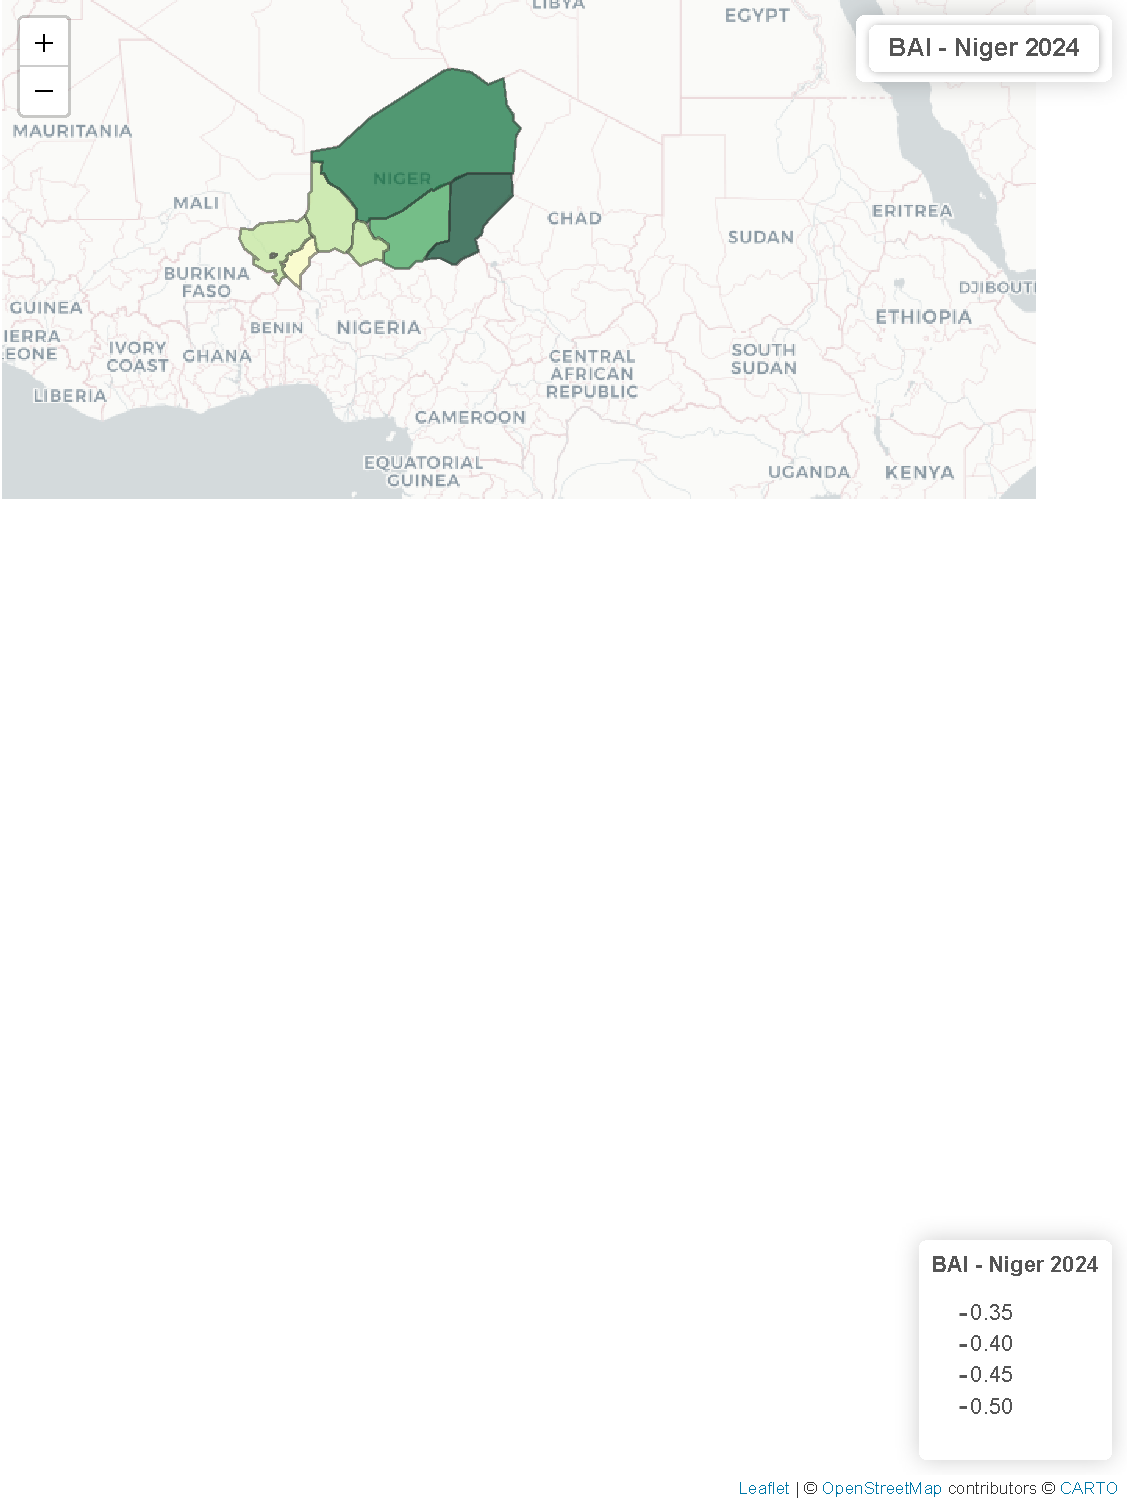
\includegraphics{Atlas-Spectral-Sahel_files/figure-latex/bai-cartes-4.pdf}

\subsection{Moyenne BAI par pays}\label{moyenne-bai-par-pays}

\begin{verbatim}
## Warning: Using `size` aesthetic for lines was deprecated in ggplot2 3.4.0.
## i Please use `linewidth` instead.
## This warning is displayed once every 8 hours.
## Call `lifecycle::last_lifecycle_warnings()` to see where this warning was
## generated.
\end{verbatim}

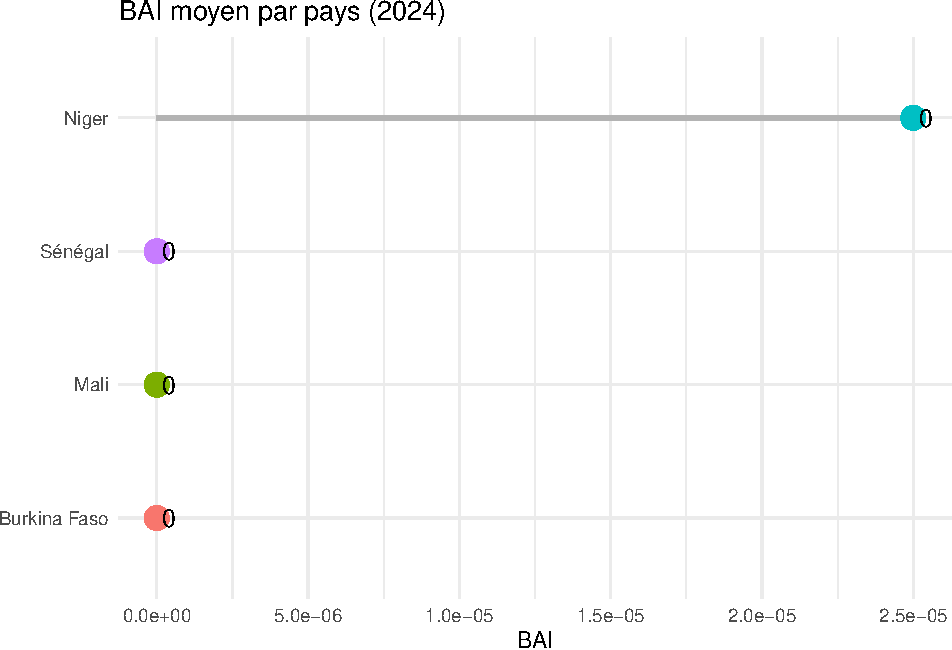
\includegraphics{Atlas-Spectral-Sahel_files/figure-latex/bai-plot-1.pdf}

\subsection{Tableau des valeurs régionales du BAI}\label{tableau-des-valeurs-ruxe9gionales-du-bai}

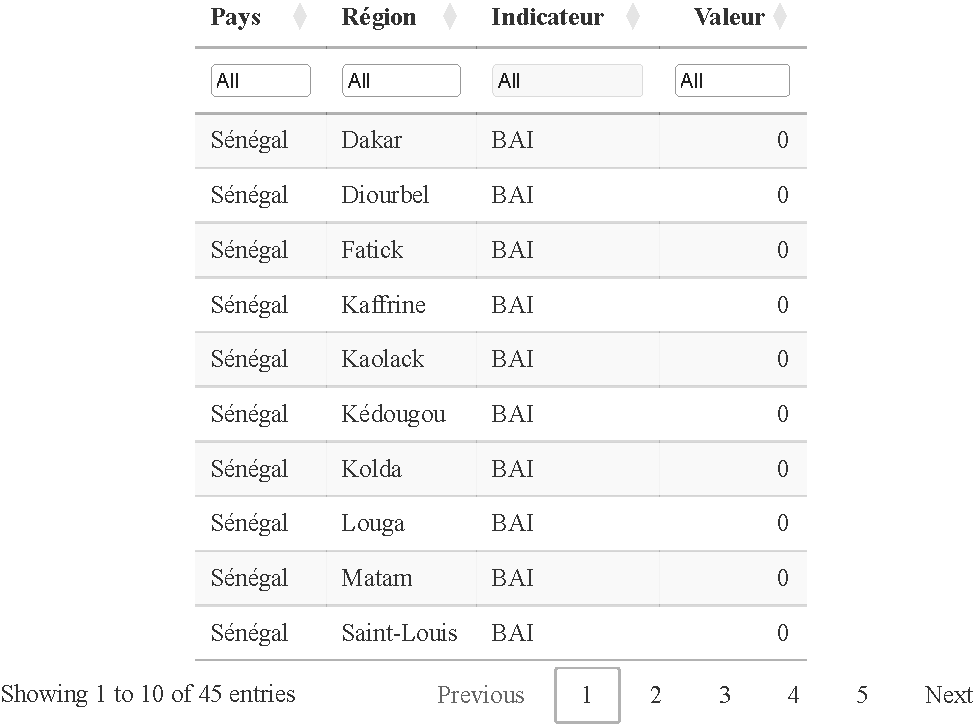
\includegraphics{Atlas-Spectral-Sahel_files/figure-latex/bai-table-1.pdf}

\subsection{🔍 Analyse comparative du stress écologique}\label{analyse-comparative-du-stress-uxe9cologique}

L'indice \textbf{BAI (Burned Area Index)} met en évidence les zones soumises à une \textbf{dégradation végétale avancée}, qu'il s'agisse de zones brûlées, de sols nus, de végétation en stress ou de perturbations écologiques diverses. Plus sa valeur est élevée, plus l'environnement est altéré ou vulnérable. Cet indice est donc un excellent proxy pour identifier les \textbf{zones écologiquement fragiles}, où la végétation est dégradée ou menacée.

\subsubsection{Lecture interne (intra-pays)}\label{lecture-interne-intra-pays-1}

À l'intérieur de chaque pays, on observe une \textbf{tendance géographique nord-sud bien marquée}, reflétant les gradients climatiques et les dynamiques d'usage des terres.

\begin{itemize}
\item
  Au \textbf{Sénégal}, le stress écologique est \textbf{modéré} dans les régions du centre-est, comme \textbf{Tambacounda} et \textbf{Matam}, mais il reste \textbf{faible dans le sud} plus humide, notamment dans les zones forestières de \textbf{Ziguinchor}.
\item
  Au \textbf{Burkina Faso}, les niveaux de BAI sont \textbf{élevés dans le Centre-Nord et la zone sahélienne}, où la pression anthropique est intense (pâturage, déforestation, agriculture extensive), tandis que les régions du sud-ouest affichent des niveaux plus faibles.
\item
  Au \textbf{Mali}, les régions \textbf{sahariennes du nord} comme \textbf{Tombouctou} ou \textbf{Kidal} présentent un \textbf{stress très élevé}, tandis que le sud agricole (ex. \textbf{Sikasso}) conserve une couverture végétale plus stable.
\item
  Au \textbf{Niger}, le \textbf{stress est généralisé} sur l'ensemble du territoire. Des valeurs élevées sont notamment observées à l'est (\textbf{Diffa}) et dans les régions désertiques du nord (\textbf{Agadez}), traduisant une forte vulnérabilité écologique.
\end{itemize}

\textbf{Conclusion intra-pays} : dans tous les pays analysés, \textbf{plus on se dirige vers le nord, plus le stress écologique augmente}. Ce phénomène s'explique par une \textbf{réduction des précipitations}, une \textbf{aridité structurelle des sols}, et des \textbf{pressions humaines accrues} dans les zones sahéliennes et désertiques.

\subsubsection{Lecture externe (inter-pays)}\label{lecture-externe-inter-pays-1}

Sur le plan comparatif, les écarts entre pays sont également significatifs :

\begin{itemize}
\item
  Le \textbf{Niger} enregistre le \textbf{BAI moyen le plus élevé}, ce qui reflète une \textbf{dégradation généralisée du couvert végétal}, accentuée par des conditions climatiques extrêmes et un contexte socio-environnemental fragile.
\item
  Le \textbf{Mali} suit, avec un niveau de stress élevé, notamment dans ses vastes zones arides du nord.
\item
  Le \textbf{Burkina Faso} présente une situation \textbf{intermédiaire}, marquée par de fortes disparités régionales, entre un nord dégradé et un sud plus résilient.
\item
  Le \textbf{Sénégal}, enfin, affiche un \textbf{stress végétal relativement faible}, notamment grâce à la \textbf{vitalité des écosystèmes du sud}, qui maintiennent une dynamique écologique plus stable.
\end{itemize}

\begin{center}\rule{0.5\linewidth}{0.5pt}\end{center}

\section{5.4 💧 Comparaison de l'humidité des surfaces}\label{comparaison-de-lhumidituxe9-des-surfaces}

L'\textbf{indice WI2 (Water Index 2)} est un indicateur spectral conçu pour mesurer la \textbf{présence d'eau ou d'humidité dans les surfaces terrestres}, qu'il s'agisse de sols, de végétation ou de plans d'eau peu profonds. Contrairement aux indices de végétation, le WI2 \textbf{ne capte pas la vigueur des plantes}, mais plutôt leur \textbf{contenu en eau} ou la \textbf{teneur en humidité résiduelle du sol}.

Un WI2 faible traduit une \textbf{situation de sécheresse ou de faible disponibilité hydrique}, tandis qu'un WI2 élevé indique une \textbf{humidité importante des surfaces}. Cet indice est donc essentiel pour détecter les zones en \textbf{stress hydrique}, et comprendre les contrastes hydrologiques dans les pays sahéliens.

\subsection{Cartes WI2 par pays}\label{cartes-wi2-par-pays}

\begin{verbatim}
## [v3->v4] `tm_raster()`: migrate the argument(s) related to the legend of the
## visual variable `col` namely 'title' to 'col.legend = tm_legend(<HERE>)'
## [v3->v4] `tm_layout()`: use `tm_title()` instead of `tm_layout(main.title = )`
\end{verbatim}

\begin{verbatim}
##   |                                                                              |                                                                      |   0%  |                                                                              |=====                                                                 |   7%  |                                                                              |==========                                                            |  14%  |                                                                              |===============                                                       |  21%  |                                                                              |====================                                                  |  29%  |                                                                              |=========================                                             |  36%  |                                                                              |==============================                                        |  43%  |                                                                              |===================================                                   |  50%  |                                                                              |========================================                              |  57%  |                                                                              |=============================================                         |  64%  |                                                                              |==================================================                    |  71%  |                                                                              |=======================================================               |  79%  |                                                                              |============================================================          |  86%  |                                                                              |=================================================================     |  93%  |                                                                              |======================================================================| 100%
\end{verbatim}

\begin{verbatim}
## Warning in pal(mean_value): Some values were outside the color scale and will
## be treated as NA
\end{verbatim}

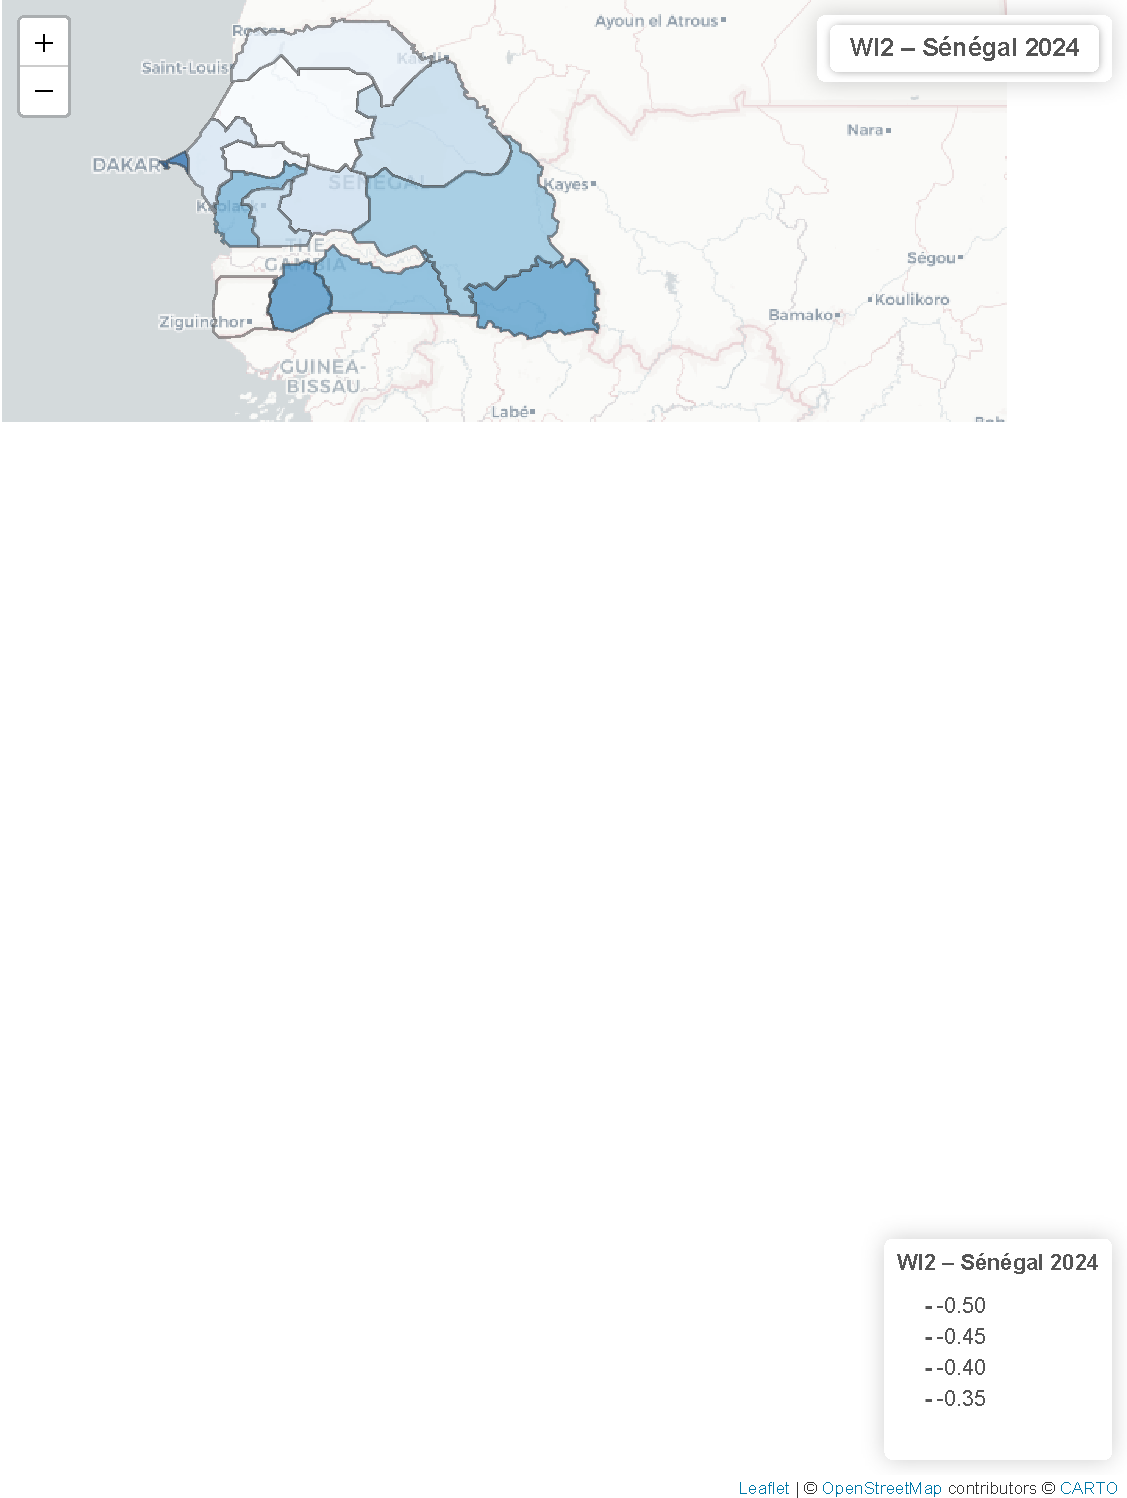
\includegraphics{Atlas-Spectral-Sahel_files/figure-latex/wi2-carte-1.pdf}

\subsection{Moyenne des valeurs du WI2 par pays}\label{moyenne-des-valeurs-du-wi2-par-pays}

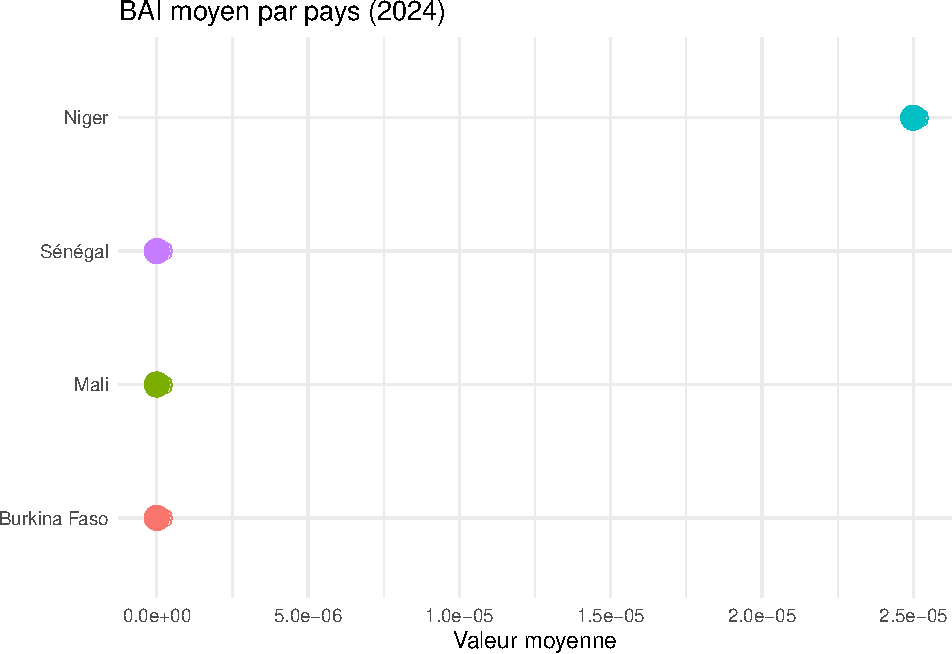
\includegraphics{Atlas-Spectral-Sahel_files/figure-latex/wi2-plot-1.pdf}

\subsection{Moyenne des tableaux du WI2 par pays}\label{moyenne-des-tableaux-du-wi2-par-pays}

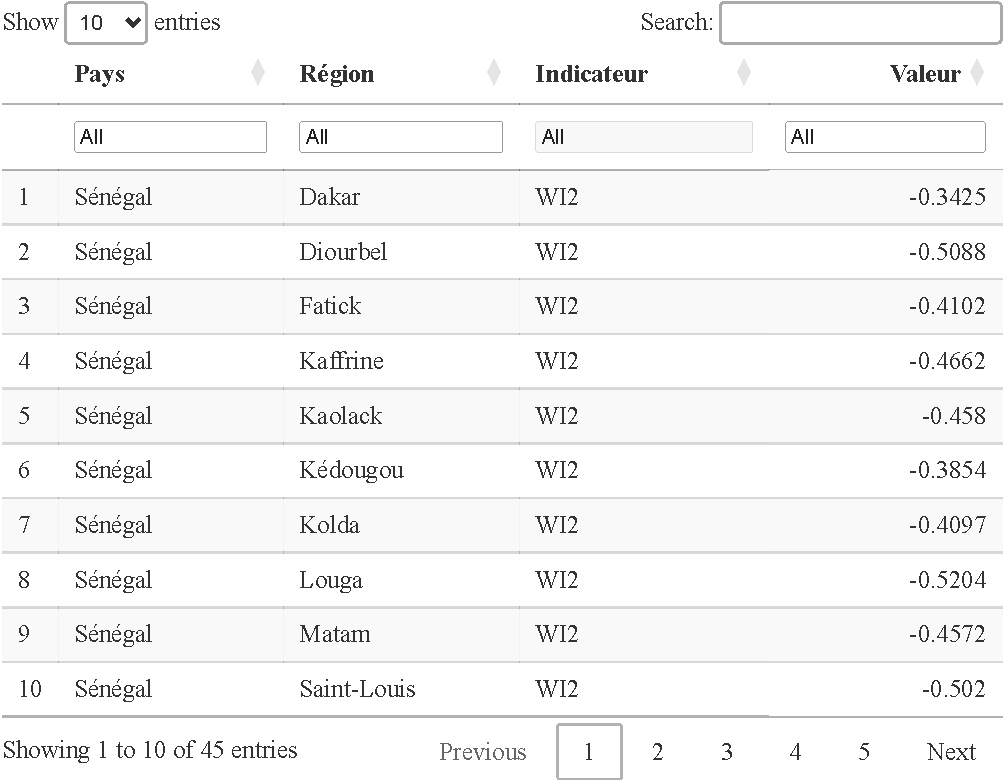
\includegraphics{Atlas-Spectral-Sahel_files/figure-latex/wi2-table-1.pdf}
\#\#\# Lecture interne (intra-pays)

À l'intérieur de chaque pays, le WI2 révèle des \textbf{disparités importantes entre les régions}, largement conditionnées par les précipitations, le couvert végétal, les sols et la topographie.

\begin{itemize}
\item
  Au \textbf{Sénégal}, les régions méridionales comme \textbf{Ziguinchor} ou \textbf{Sédhiou} présentent des WI2 nettement plus élevés, en lien avec la forte pluviométrie, la densité végétale et la présence de zones humides (bolongs, rizières). À l'inverse, les régions sahéliennes du nord (Saint-Louis, Louga) affichent des niveaux d'humidité faibles.
\item
  Au \textbf{Burkina Faso}, une humidité relative est conservée dans les régions du \textbf{Sud-Ouest}, des \textbf{Cascades} et des \textbf{Hauts-Bassins}, tandis que le Centre-Nord et le Sahel sont beaucoup plus secs.
\item
  Au \textbf{Mali}, on observe une structure similaire : \textbf{le sud (Sikasso, Koulikoro)} concentre l'essentiel de l'humidité résiduelle, alors que les zones sahariennes (Tombouctou, Kidal) restent extrêmement sèches, avec des WI2 très bas.
\item
  Au \textbf{Niger}, l'humidité est faible de manière généralisée. Les \textbf{régions de Maradi, Dosso ou Tillabéri} présentent des valeurs légèrement meilleures, mais le reste du territoire affiche une situation hydrique préoccupante, en particulier à l'est (Diffa) et au nord désertique (Agadez).
\end{itemize}

\textbf{Conclusion intra-pays} : dans tous les pays, l'humidité des surfaces \textbf{décroît progressivement du sud vers le nord}, en lien direct avec la baisse des précipitations, la réduction du couvert végétal et la structure climatique zonale.

\begin{center}\rule{0.5\linewidth}{0.5pt}\end{center}

\subsection{Lecture externe (inter-pays)}\label{lecture-externe-inter-pays-2}

La comparaison des WI2 moyens entre pays permet d'identifier les territoires les \textbf{plus exposés à la sécheresse} :

\begin{itemize}
\item
  Le \textbf{Niger} est, sans surprise, le pays avec le \textbf{WI2 le plus faible}, confirmant son exposition structurelle à l'aridité et sa très faible disponibilité en eau de surface.
\item
  Le \textbf{Mali} et le \textbf{Burkina Faso} se situent dans une zone intermédiaire, avec des contrastes marqués selon les régions, mais une vulnérabilité réelle au stress hydrique.
\item
  Le \textbf{Sénégal} présente le \textbf{WI2 moyen le plus élevé}, grâce aux écosystèmes du sud qui conservent une humidité résiduelle importante, malgré un nord plus sec.
\end{itemize}

\textbf{Conclusion inter-pays} : parmi les pays analysés, le \textbf{Sénégal bénéficie d'un avantage hydrique relatif}, tandis que le \textbf{Niger cumule faiblesse du couvert végétal et déficit hydrique}, faisant de lui le territoire le plus fragile sur le plan agro-hydrologique.

\begin{center}\rule{0.5\linewidth}{0.5pt}\end{center}

\section{Conclusion}\label{conclusion-4}

Ce chapitre a permis de dresser un portrait comparatif des dynamiques environnementales dans quatre pays de la bande sahélienne ouest-africaine : Sénégal, Burkina Faso, Mali et Niger. En mobilisant des indicateurs spectraux harmonisés (NDVI, BAI, WI2), nous avons mis en évidence les contrastes écologiques majeurs, tant à l'intérieur de chaque pays qu'entre eux.

Sur le plan de la végétation active (NDVI), le Sénégal et le Burkina Faso apparaissent comme les territoires les plus densément végétalisés, notamment dans leurs régions méridionales. À l'opposé, le Niger et le Mali, confrontés à une aridité plus prononcée, affichent une végétation plus clairsemée, avec une prédominance de zones semi-arides voire désertiques au nord.

Concernant le stress écologique (BAI), les cartes et les valeurs moyennes révèlent une vulnérabilité croissante vers le nord dans tous les pays. Le Niger se distingue par une dégradation généralisée du sol et de la couverture végétale, traduisant à la fois les effets du climat et des pressions humaines. Le Sénégal, en revanche, présente une meilleure résilience écologique, surtout dans ses zones humides du sud.

Enfin, l'analyse de l'humidité des surfaces (WI2) montre des gradients similaires. Le Sénégal bénéficie d'un profil hydrique relativement favorable grâce à ses zones fluviales et forestières. Le Burkina Faso et le Mali présentent des contrastes internes forts, tandis que le Niger concentre les plus faibles niveaux d'humidité, confirmant sa forte exposition au stress hydrique.

\begin{quote}
\emph{``Comparer les espaces, c'est comprendre les trajectoires. Et comprendre, c'est déjà agir.''}
\end{quote}

\end{document}
